% Última edición: 05/06/2023

\documentclass[12pt]{report}

\usepackage{graphicx}
\usepackage[a4paper, total={6.5in, 9in}]{geometry}
\usepackage[utf8]{inputenc}
\usepackage[spanish]{babel}
\usepackage{amsmath,amsfonts,amssymb,amsthm}
\usepackage{hyperref} % Para poder insertar hiperenlaces a secciones del documento
\usepackage[table, x11names]{xcolor} % Para cambiar las letras de color
\usepackage{dirtytalk} % Para usar comillas de apertura y cierre
\usepackage{fbox} % Para las cajas en las demostraciones de "si y solo si" y doble contención
\usepackage{mathtools}
\usepackage{multicol} % Para dividir una lista en varias columnas
\usepackage{soul} % Para cambiar de línea con palabras subrayadas
\usepackage{imakeidx}
\usepackage{graphicx}
\usepackage{faktor} % Conjuntos cociente
\usepackage{float} % Para que algunas figuras no se coloquen al inicio de la página
\usepackage{centernot} % Para negar símbolos como \implies
\usepackage{soulutf8} % Para pegar el subrayado al texto
\usepackage{esvect}
\usepackage{spalign}
\usepackage{array}

\makeindex[columns=3, intoc]

\setlength{\columnsep}{0.8cm} % Recta que separa dos columnas (multicols)
\setlength{\columnseprule}{1.5pt}

\makeatletter % Para que el título de los teoremas estén en negrita
\def\th@plain{%
  \thm@notefont{}
  \itshape
}
\def\th@definition{
  \thm@notefont{}
  \normalfont
}
\makeatother

\graphicspath{{./images/}}

\newtheorem{proposition}{Proposición}[chapter]
\newtheorem{corollary}{Corolario}[chapter]
\newtheorem{theorem}{Teorema}[chapter]
\theoremstyle{definition}
\newtheorem{definition}{Definición}[chapter]
\theoremstyle{definition}
\newtheorem{example}{Ejemplo}[chapter]
\theoremstyle{remark}
\newtheorem*{obs}{Observación} % * para que no se numeren
\renewcommand*{\proofname}{Demostración}
\setcounter{chapter}{-1} % Para que el primer tema sea el Tema 0 y no el Tema 1
\addto\captionsspanish{\renewcommand{\chaptername}{Tema}} % Para que ponga "Tema 1" en vez de "Capítulo 1"
\addto\captionsspanish{\renewcommand{\contentsname}{Índice}} % Para cambiar el título del índice

\setuldepth{Berlin}

\newcommand*{\Scale}[2][4]{\scalebox{#1}{$#2$}}%

% Shortcuts:
\newcommand{\R}{\mathbb R}
\newcommand{\N}{\mathbb N}
\newcommand{\Z}{\mathbb Z}
\newcommand{\Q}{\mathbb Q}

\begin{document}

% Longitud antes y después de una expresión matemática:
\setlength{\abovedisplayskip}{10pt}
\setlength{\belowdisplayskip}{10pt}

\thispagestyle{empty} % Ocultar el contador de páginas pero seguir contando

\begin{center}
    \vspace*{1cm} % Sin el asterisco, \vspace se ignora al principio del documento
    \Huge \textbf{Ampliación de \\ Álgebra Lineal y Geometría}
        
    \vspace{10mm} % \vspace tiene que estar separado de la línea anterior para que funcione
    \large
%    David López
        
%    \vspace{5mm}
    Curso 2022-2023
\end{center}

\tableofcontents

\addtocontents{toc}{\protect\thispagestyle{empty}} % Para que no se numeren las páginas del índice
\pagenumbering{gobble}

\chapter{Espacios vectoriales}

\pagenumbering{arabic}
\setcounter{page}{4}

Gran parte de este tema ya se vio en la asignatura \textit{Álgebra Lineal y Geometría}. Se omitirán las demostraciones de la mayoría de los resultados y las definiciones de algunos conceptos básicos.

\begin{definition}
Sea $\mathbb K$ un cuerpo y sea $V$ un conjunto no vacío. Diremos que $V$ es un \ul{espacio vectorial} sobre $\mathbb K$ si
\begin{itemize}
    \item[I.] En $V$ hay definida una operación interna, que denotaremos por $+$, de forma que $(V,+)$ verifica las siguientes propiedades:
    \begin{itemize}
        \item[(i)] $(u+v)+w=u+(v+w) \ \forall \  u,v,w \in V$.
        \item[(ii)] $u+v=v+u \ \forall \  u,v \in V$.
        \item[(iii)] $\exists \ 0 \in V$ tal que $v+0=0+v=v \ \forall \ v \in V$.
        \item[(iv)] $\forall \  v \in V,\  \exists \ -v \in V$ tal que $v+(-v)=(-v)+v=0$.
    \end{itemize}
    \item[II.] En $V$ hay definida una operación externa de $\mathbb K$ en $V$, que denotaremos por yuxtaposición, verificando
    \begin{itemize}
        \item[(i)] $\lambda(u+v)=\lambda u+\lambda v \ \forall \ \lambda \in \mathbb K, \ \forall \ u,v \in V$.
        \item[(ii)] $(\lambda+\mu)u=\lambda u + \mu u \ \forall \ \lambda,\mu \in \mathbb K, \ \forall \ u \in V$.
        \item[(iii)] $\lambda(\mu u)=(\lambda \mu)u \ \forall \ \lambda,\mu \in \mathbb K, \ \forall \ u \in V$.
        \item[(iv)] $1 u = u \ \forall \ u \in V$, donde $1$ es la unidad para el producto en $\mathbb K$.
    \end{itemize}
\end{itemize}
\end{definition}

\section{Ecuaciones de subespacio}

\begin{definition}
Sea $V$ un espacio vectorial sobre $\mathbb K$ y sea $U \subset V$ no vacío. Decimos que $U$ es un \ul{subespacio vectorial} de $V$, y lo denotamos por $U \leq V$, cuando se verifican las siguientes propiedades:
\begin{itemize}
    \item[(i)] $U$ es cerrado para la suma: $u+v \in U \ \forall \ u,v \in U$.
    \item[(ii)] $U$ es cerrado para el producto por escalares: $\lambda u \in U \ \forall \ \lambda \in \mathbb K, \ \forall \ u \in U$.
\end{itemize}
\end{definition}

En este apartado veremos las distintas formas de determinar un subespacio vectorial $U$ mediante un sistema de ecuaciones lineales. Sea $V$ un espacio vectorial sobre el cuerpo $\mathbb K$ y sea $\mathcal{B} = \{e_1,\mathellipsis,e_n\}$ una base de $V$. Sea $U =\ <u_1,\mathellipsis,u_k>$ ($k \leq n$) un subespacio vectorial de $V$. Dado $v \in U$, existen $\lambda_1,\mathellipsis,\lambda_k \in \mathbb K$ tales que
\[v = \lambda_1 u_1+\mathellipsis \lambda_k u_k\]
Esta ecuación se denomina \ul{ecuación vectorial} de $U$.

\vspace{2mm}
Por otro lado, los elementos del sistema de generadores de $U$ se pueden escribir de la siguiente forma:
\[
\begin{cases}
    u_1 = a_{11}e_1+a_{12}e_2+\mathellipsis+a_{1n}e_n = (a_{11},\mathellipsis,a_{1n})_{\mathcal{B}}\\
    u_2 = a_{21}e_1+a_{22}e_2+\mathellipsis+a_{2n}e_n = (a_{21},\mathellipsis,a_{2n})_{\mathcal{B}}\\
   \ \vdots \\
    u_k = a_{k1}e_1+a_{k2}e_2+\mathellipsis+a_{kn}e_n = (a_{k1},\mathellipsis,a_{kn})_{\mathcal{B}}
\end{cases}
\]
Dado $v =(x_1,\mathellipsis,x_n) \in U$, se tiene que
\[v = \lambda_1u_1 + \lambda_2u_2 \mathellipsis + \lambda_ku_k = \lambda_1(a_{11},\mathellipsis,a_{1n})_{\mathcal{B}} +\lambda_2(a_{21},\mathellipsis,a_{2n})_{\mathcal{B}} +\mathellipsis +\lambda_k(a_{k1},\mathellipsis,a_{kn})_{\mathcal{B}}\]
Por tanto,
\[
\begin{cases}
    x_1 = \lambda_1a_{11}+\lambda_2a_{21}+\mathellipsis+\lambda_ka_{k1} \\
    x_2 = \lambda_1a_{12}+\lambda_2a_{22}+\mathellipsis+\lambda_ka_{k2} \\
    \ \vdots \\
    x_n=\lambda_1a_{1n}+\lambda_2a_{2n}+\mathellipsis+\lambda_ka_{kn}
\end{cases}
\]
Las $n$ ecuaciones anteriores son las \ul{ecuaciones paramétricas} de $U$.

\vspace{2mm}
Veamos, por último, cómo obtener las ecuaciones cartesianas de $U$. Para que un vector $v = (x_1,x_2\mathellipsis,x_n)\in V$ esté en $U$, la matriz
\[
\begin{pmatrix*}[r]
u_1 & u_2 & \mathellipsis & u_k & v
\end{pmatrix*}
=
\begin{pmatrix*}[r]
a_{11} & a_{21} & \mathellipsis & a_{k1} & x_1 \\
a_{12} & a_{22} & \mathellipsis & a_{k2} & x_2 \\
\vdots & \vdots & \ddots & \vdots & \vdots \\
a_{1n} & a_{2n} & \mathellipsis & a_{kn} & x_n
\end{pmatrix*}
\]
debe tener rango $k$. Por tanto, todos los menores de orden $k+1$ deben ser $0$, lo que nos proporciona un sistema homogéneo de $n-k$ ecuaciones en las incógnitas $x_1,x_2,\mathellipsis,x_n$ que es verificado por las coordenadas de cualquier vector de $U$. Estas $n-k$ ecuaciones son las \ul{ecuaciones cartesianas} de $U$.

\begin{example}
En $\R^4$, tomemos $U = \ <(1,1,0,0),(1,0,1,0),(1,0,0,1)>$. Entonces $v \in U$ si y solo si
\[v = \lambda_1(1,1,0,0)+\lambda_2(1,0,1,0)+\lambda_3(1,0,0,1), \quad \lambda_1, \lambda_2, \lambda_3 \in \R\]
Esta es la ecuación vectorial de $U$. Además, si llamamos $\mathcal{B}' = \{(1,1,0,0),(1,0,1,0),(1,0,0,1)\}$, entonces $v$ tiene coordenadas $(\lambda_1,\lambda_2,\lambda_3)_{\mathcal{B}'}$ en la base $\mathcal{B}'$ de $U$. También podemos escribir
\[v = (\lambda_1+\lambda_2+\lambda_3,\lambda_1,\lambda_2,\lambda_3)\]
así que las ecuaciones paramétricas de $U$ son
\[
\begin{cases}
    x_1 = \lambda_1+\lambda_2+\lambda_3 \\
    x_2 = \lambda_1 \\
    x_3 = \lambda_2 \\
    x_4 = \lambda_3
\end{cases}
\]
Si $v = (x_1,x_2,x_3,x_4)$, entonces
\[
\begin{pmatrix*}[r]
    1 & 0 & 0 & 1 \\
    0 & 1 & 0 & -1 \\
    0 & 0 & 1 & -1 \\
    x_1 & x_2 & x_3 & x_4 
\end{pmatrix*}
\ \overset{\textrm{\scriptsize Gauss}}{\Scale[2.5]{\sim}} \
\begin{pmatrix*}[r]
    1 & 0 & 0 & 1 \\
    0 & 1 & 0 & -1 \\
    0 & 0 & 1 & -1 \\
    0 & 0 & 0 & x_4-x_1+x_2+x_3
\end{pmatrix*}
\]
Para que el rango de esta última matriz sea $3$ debe cumplirse que
\[
\begin{cases}
    x_4-x_1+x_2+x_3=0
\end{cases}\]
Esta es la ecuación cartesiana de $U$.
\end{example}

\begin{example}
Vamos a pasar de ecuaciones cartesianas a ecuaciones paramétricas. Sea $W$ el subespacio dado por las ecuaciones
\[
\spalignsys{
x_1 - x_2 + x_3 - x_4 = 0 ;
x_1 + x_2 + x_3 + x_4 = 0 ;
2x_1 \. \+ + 2x_3 \. \+ = 0
}
\]
\[
\begin{pmatrix*}[r]
    1 & -1 & 1 & -1 \\
    1 & 1 & 1 & 1 \\
    2 & 0 & 2 & 0
\end{pmatrix*}
\ \overset{\textrm{\scriptsize Gauss}}{\Scale[2.5]{\sim}} \
\begin{pmatrix*}[r]
    1 & 0 & 1 & 0 \\
    0 & 1 & 0 & 1 \\
    0 & 0 & 0 & 0
\end{pmatrix*}
\]
$W$ también viene dado por las ecuaciones
\[
\begin{cases}
    x_1+x_3=0 \\
    x_2+x_4=0
\end{cases}
\]
Por tanto, las ecuaciones paramétricas son
\[
\begin{cases}
    x_1=-\lambda \\
    x_2=-\mu \\
    x_3 = \lambda \\
    x_4 = \mu
\end{cases}
\]
\end{example}

\section{Retículo de subespacios}

\begin{definition}
    Un \ul{retículo} es un conjunto parcialmente ordenado $(X, \leq)$ de forma que para cada par $\{a,b\}$ existen $\sup(\{a,b\})$ e $\inf(\{a,b\})$.
\end{definition}

Se recuerda que una relación $\leq$ es una \ul{relación de orden} si verifica las propiedades reflexiva, transitiva y antisimétrica. Se dice que $\leq$ es un \ul{orden parcial} si no necesariamente debe poder compararse todo par de elementos del conjunto, es decir, si no es un orden total.

\begin{proposition}
Sea $V$ un espacio vectorial. Entonces
\[S(V)=\{U \subset V \colon U \textrm{es subespacio de } V\}\]
es un retículo para la relación de orden $U \leq W \iff U \subset W$. Además,
\[\sup(\{U,W\}) = U+W \qquad \inf(\{U,W\}) = U \cap W\]
\end{proposition}

En la práctica, la suma $U + W$ puede hallarse reuniendo las bases de ambos subespacios y eliminando los vectores linealmente dependientes, mientras que $U \cap W$ puede hallarse reuniendo las ecuaciones cartesianas de ambos subespacios y elimiando aquellas que sean combinaciones lineales de otras.

\begin{example}
En $\R^4$, sea $U = \ <(1,0,-1,0),(2,0,0,-1)>$ y sea $W$ el subespacio dado por
\[
\spalignsys{
x_1 + x_2 + 2x_3 + x_4 = 0 ;
\. \+ \. - x_3 + x_4 = 0
}\]
Calculemos $U + W$. Hay que hallar una base de $W$. Las ecuaciones paramétricas de $W$ son
\[
\begin{cases}
    x_1=-\lambda-3\mu \\
    x_2=\lambda \\
    x_3 = \mu \\
    x_4 = \mu
\end{cases}
\]
luego $W = \ <(-1,1,0,0),(-3,0,1,1)>$. Por tanto,
\[U+W= \ <(1,0,-1,0),(2,0,0,-1),(-1,1,0,0),(-3,0,1,1)>\]
Ahora hay que transformar el sistema de generadores anterior en una base.
\[
\begin{pmatrix*}[r]
    1 & 0 & -1 & 0 \\
    2 & 0 & 0 & -1 \\
    -1 & 1 & 0 & 0 \\
    -3 & 0 & 1 & 1
\end{pmatrix*}
\ \overset{\textrm{\scriptsize Gauss}}{\Scale[2.5]{\sim}} \
\begin{pmatrix*}[r]
    1 & 0 & 0 & -1/2 \\
    0 & 1 & 0 & -1/2 \\
    0 & 0 & 1 & -1/2 \\
    0 & 0 & 0 & 0
\end{pmatrix*}
\]
Por tanto,
\[U+W = \ <(1,0,0,-1/2),(0,1,0,-1/2),(0,0,1,-1/2)>\]
\end{example}

\begin{theorem}[Fórmula de Grassmann]
Sea $V$ un espacio vectorial y sean $U,W \leq V$. Entonces
\[\dim(U+W)=\dim(U)+\dim(W)-\dim(U \cap W)\]
\end{theorem}

\begin{definition}
Sea $V$ un espacio vectorial y sean $U,W \leq V$. Se dice que la suma $U+W$ es \ul{directa}, y se denota $U \oplus W$, cuando $U \cap W = \{0\}$, o lo que es lo mismo, cuando 
\[\dim(U+W)=\dim(U)+\dim(W)\]
\end{definition}

\section{Aplicaciones lineales}

\begin{definition}
Sean $V$, $V'$ espacios vectoriales sobre el mismo cuerpo $\mathbb{K}$. Una aplicación $f \colon V \to V'$ se dice que es una \ul{aplicación lineal} si verifica
\begin{itemize}
    \item[(i)] $f(\lambda v) = \lambda f(v) \ \forall \ \lambda \in \mathbb{K}, \ \forall \ v \in V$.
    \item[(ii)] $f(u+v)=f(u)+f(v) \ \forall \ u,v \in V$.
\end{itemize}
\end{definition}

Nótese que estas dos condiciones son equivalentes a que para todos $\lambda,\mu \in \mathbb{K}, u,v \in V$ se tenga que $f(\lambda u + \mu v) = \lambda f(u) + \mu f(v)$, y esto, a su vez, equivale a que se cumpla $f(\lambda u + v) = \lambda f(u) + f(v) \ \forall \ \lambda \in \mathbb{K}, \, \forall \ u,v \in V$.


\begin{proposition}
Una aplicación lineal $f \colon V \to V'$ queda totalmente determinada por la imagen de una base de $V$.
\end{proposition}

Sea $f \colon V \to V'$ una aplicación lineal y tomemos bases $\mathcal{B} = \{e_1,\mathellipsis,e_n\}$, $\mathcal{B}' = \{e_1',\mathellipsis,e_m'\}$ de $V$ y $V'$, respectivamente. Para todo $i = 1, \mathellipsis, n$ el vector $f(e_i)$ tiene coordenadas 
\[f(e_i) = (a_{i1},\mathellipsis,a_{im})_{\mathcal{B'}}\]
en la base $B'$. La matriz
\[A = \begin{pmatrix*}[r]
f(e_1) & \mathellipsis & f(e_n)
\end{pmatrix*}
=
\begin{pmatrix*}[r]
a_{11} & a_{21} & \mathellipsis & a_{n1} \\
a_{12} & a_{22} & \mathellipsis & a_{n2} \\
\vdots & \vdots & \ddots & \vdots \\
a_{1m} & a_{2m} & \mathellipsis & a_{nm}
\end{pmatrix*}\]
de orden $m \times n$ es la \ul{matriz de la aplicación lineal $f$} respecto de las bases $\mathcal{B}$ y $\mathcal{B}'$, y se denota $A = \mathcal{M}_{\mathcal{B},\mathcal{B}'}(f)$. Si tomamos $v \in V$ y las coordenadas de $v$ y $f(v)$ respecto de las bases $\mathcal{B}$ y $\mathcal{B'}$ son, respectivamente,
\[v = (x_1,\mathellipsis,x_n)_{\mathcal{B}} \qquad f(v) = (y_1,\mathellipsis,y_n)_{\mathcal{B}'}\]
entonces se tiene que
\[\begin{pmatrix*}[r]
a_{11} & a_{21} & \mathellipsis & a_{n1} \\
a_{12} & a_{22} & \mathellipsis & a_{n2} \\
\vdots & \vdots & \ddots & \vdots \\
a_{1m} & a_{2m} & \mathellipsis & a_{nm}
\end{pmatrix*}
\begin{pmatrix*}[r]
    x_1 \\
    x_2 \\
    \vdots \\
    x_n
\end{pmatrix*} =
\begin{pmatrix*}[r]
    y_1 \\
    y_2 \\
    \vdots \\
    y_n
\end{pmatrix*}
\iff Av = f(v)
\]

En el teorema que sigue se recogen varias propiedades importantes de las aplicaciones lineales.

\begin{theorem}
Sean $V,V'$ espacios vectoriales y sea $f \colon V \to V'$ aplicación lineal. Entonces
\begin{itemize}
    \item[(i)] $\mathrm{Ker} (f) = \{v \in V \colon f(v)=0\}$ es un subespacio vectorial de $V$.
    \item[(ii)] $\mathrm{Im} (f) = \{f(v) \in V' \colon v \in V\}$ es un subespacio vectorial de $V'$.
    \item[(iii)] $f$ es inyectiva si y solo si $\mathrm{Ker} (f) = \{0\}$, o lo que es lo mismo, $f$ es inyectiva si y solo si $f$ envía vectores independientes en vectores independientes.
    \item[(iv)] Si $\mathrm{dim}(V)=\mathrm{dim}(V')$, entonces $f$ es inyectiva si y solo si $f$ es sobreyectiva.
    \item[(v)] Si llamamos $A = \mathcal{M}_{\mathcal{B},\mathcal{B}'}(f)$, entonces $\mathrm{dim}(\mathrm{Im}(f)) = \mathrm{rg(A)}$.
    \item[(vi)] $f$ es isomorfismo si y solo si $A$ es inversible.
\end{itemize}
\end{theorem}

\section{Espacios duales}

\begin{definition}
Sea $V$ espacio vectorial sobre el cuerpo $\mathbb{K}$. Una \ul{forma lineal} es una aplicación lineal $f \colon V \to \mathbb{K}$.
\end{definition}

\begin{example}
Sea $f \colon \R^3 \to \R$ definida por $f(x,y,z) = 2x+y+z$. Entonces $f$ es una forma lineal.
\end{example}

La interpretación geométrica del concepto de forma lineal es que cada forma lineal captura un hiperplano de $V$ vía $\mathrm{Ker}(f)$.

\begin{definition}
Sea $V$ espacio vectorial sobre el cuerpo $\mathbb{K}$. El \ul{espacio dual} de $V$ es el siguiente espacio vectorial sobre $\mathbb{K}$:
\[V^* = \{f \colon V \to \mathbb{K} \mid f \textrm{ es forma lineal}\} = \mathrm{Hom}_{\mathbb{K}}(V,\mathbb{K})\]
Las operaciones de dicho espacio vectorial son 
\begin{equation*}
\begin{aligned}[t]
f+g \colon V &\longrightarrow \mathbb{K} \\
v &\longmapsto (f+g)(v) = f(v)+g(v)
\end{aligned}
\qquad
\begin{aligned}[t]
\lambda f \colon V &\longrightarrow \mathbb{K} \\
v &\longmapsto \lambda f(v) = \lambda f(v)
\end{aligned}
\end{equation*}
para todas $f,g \in V^*$ y para todo $\lambda \in \mathbb{K}$.
\end{definition}

\begin{theorem}
Sea $\mathcal{B} = \{e_1,\mathellipsis,e_n\}$ una base del espacio vectorial $V$. Entonces el conjunto $\mathcal{B}^* = \{f_1,\mathellipsis,f_n\}$ de formas lineales dadas por
\[f_i(e_j) = \begin{cases}
1 & $si$ \ i = j \\
0 & $si$ \ i \neq j
\end{cases}\]
es una base de $V^*$.
\end{theorem}

En consecuencia, la aplicación $F \colon V \to V^*$ dada por $F(e_i)=f_i$ para cada $i = 1,\mathellipsis,n$ es isomorfismo, con inversa $F^{-1} \colon V^* \to V$ dada por $F^{-1}(f_i)=e_i$ para cada $i = 1,\mathellipsis,n$.

\begin{example}
    Sea $\mathcal{B} = \{(1,-2),(3,4)\}$ una base de $\R^2$ y calculemos $\mathcal{B}^*$. Sean $\phi_1,\phi_2 \colon \R^2 \to \R$ tales que
    \[\phi_1(x,y)=a_{11}x+a_{12}y\]
    \[\phi_2(x,y)=a_{21}x+a_{22}y\]
    Debe cumplirse que
    \[
    \begin{cases}
        \phi_1(1,-2)=1 \\
        \phi_1(3,4)=0
    \end{cases}
    \iff
    \begin{cases}
        a_{11}-2a_{12} = 1 \\
        3a_{11}+4a_{12}=0
    \end{cases}
    \iff
    a_{11}=\frac{2}{5}, \, a_{12}=-\frac{3}{10}
    \]
    \[
    \begin{cases}
        \phi_2(1,-2)=0 \\
        \phi_2(3,4)=1
    \end{cases}
    \iff
    \begin{cases}
        a_{21}-2a_{22} = 0 \\
        3a_{21}+4a_{22}=1
    \end{cases}
    \iff
    a_{21}=\frac{1}{5}, \, a_{22}=\frac{1}{10}
    \]
    Por tanto,
    \[\phi_1(x,y)=\frac{2}{5}x-\frac{3}{10}y\]
    \[\phi_2(x,y)=\frac{1}{3}x+\frac{1}{10}y\]
    y $\mathcal{B}^* = \{\phi_1,\phi_2\}$ es la base dual de $\mathcal{B} = \{e_1,e_2\}$.
\end{example}

\section{Anuladores}

\begin{definition}
Sea $U$ un subconjunto (no necesariamente subespacio) de un espacio vectorial $V$. Se define el \ul{anulador} de $U$, y se denota $U^\circ$, como
\[U^\circ = \{f \in V^* \colon f(u)=0 \ \forall \ u \in U\}\]
ó bien $U^\circ = V^*$ en caso de que sea $U = \emptyset$.
\end{definition}

Las propiedades más importantes relacionadas con anuladores se recogen en el siguiente teorema:

\begin{theorem}
\label{teo0.4.}
    Sea $U$ un subconjunto del espacio vectorial $V$. Entonces
    \begin{itemize}
        \item[(i)] $U^\circ$ es un subespacio de $V^*$.
        \item[(ii)] Tomar anuladores invierte inclusiones, es decir, si $U \subset W$, entonces $W^\circ \subset U^\circ$.
        \item[(iii)] Si $\{u_1,\mathellipsis,u_k\}$ es una base de $U$ y $f \in V^*$, entonces $f \in U^\circ$ si y solo si $f(u_i)=0$ para todo $i = 1,\mathellipsis,k$.
        \item[(iv)] Sea $\mathcal{B} = \{e_1,\mathellipsis,e_n\}$ una base de $V$ con base dual $B^* = \{f_1,\mathellipsis,f_n\}$ y sea $\{u_1,\mathellipsis,u_k\}$ una base de $U$. Si para cada $i = 1,\mathellipsis,k$ escribimos $u_i = (a_{i1},\mathellipsis,a_{in})_\mathcal{B}$, entonces las ecuaciones cartesianas de $U^\circ$ son
        \[
        \begin{cases}
            a_{11}x_1+\mathellipsis+a_{1n}x_n = 0 \\
            a_{21}x_1+\mathellipsis+a_{2n}x_n = 0 \\
            \ \vdots \\
            a_{k1}x_1+\mathellipsis+a_{kn}x_n = 0
        \end{cases}
        \]
        \item[(v)] Tomar anuladores induce una inyección de $S(V)$ en $S(V^*)$ que envía cada $U \in S(V)$ a $U^\circ \in S(V^*)$.
        \item[(vi)] Tomar anuladores intercambia sumas e intersecciones, es decir, $(U+W)^\circ = U^\circ \cap W^\circ$ y $(U \cap W)^\circ = U^\circ + W^\circ$.
    \end{itemize}
\end{theorem}

\begin{example}
     Sea $\mathcal{B}$ la base canónica del espacio vectorial $V=\R^4$, con base dual $\mathcal{B^*}$, y tomemos $U = \ <u_1=(1,1,0,0), \, u_2=(1,0,1,0)>$. Por la proposición anterior, las ecuaciones cartesianas de $U^\circ$ son
     \[
     \begin{cases}
         x_1+x_2=0 \\
         x_1+x_3=0
     \end{cases}
     \]
     La solución del sistema es
     \[(x_1,x_2,x_3,x_4)=\lambda_1 (-1,1,1,0)+\lambda_2(0,0,0,1)\]
     Por tanto, las formas lineales
     \[\phi_1 = (-1,1,1,0)_{\mathcal{B}^*} = -f_1+f_2+f_3, \ \phi_2 = (0,0,0,1)_{\mathcal{B}^*} = f_1\]
     constituyen una base de $U$, así que $U^\circ = \ <\phi_1,\phi_2>$.
\end{example}

Se trata ahora de definir el anulador de un subespacio del espacio dual $V^*$, en lugar del espacio vectorial $V$. En el caso de $V$, se podía definir el anulador de un subconjunto cualquiera de $V$, pero en el espacio dual se necesitará que el subconjunto de $V^*$ en cuestión sea un subespacio vectorial.

\begin{definition}
Sea $W \leq V^*$ un subespacio vectorial del espacio dual $V^*$. Se define el anulador de $W$, y se denota por $W^\circ$, como
\[W^\circ = \bigcap_{f \in W}\mathrm{Ker}(f) = \{v \in V \colon f(v) = 0 \ \forall \ f \in W\}\]
\end{definition}

Nótese que si $W \leq V^*$, entonces $(W^\circ)^\circ = W$, y si $U \leq V$, entonces $(U^\circ)^\circ = U$. En esta última igualdad, tiene sentido considerar el anulador de $U^\circ$ porque, como se vio en el teorema anterior, $U^\circ$ es un subespacio de $V^*$. 

\chapter{Espacios afines y proyectivos}

\section{Introducción}

\begin{definition}
Dado un vector $a$ de un espacio vectorial $V$ sobre el cuerpo $\mathbb{K}$, a la aplicación $\tau_a \colon V \to V$ dada por $\tau_a(v) = v+a$ se le denomina \ul{traslación}.
\end{definition}

\begin{proposition}
Sea $V$ un espacio vectorial sobre el cuerpo $\mathbb{K}$. Se tiene que
\begin{itemize}
    \item[(i)] Las traslaciones son aplicaciones biyectivas.
    \item[(ii)] $\tau_a \circ \tau_b = \tau_{a+b}$.
    \item[(iii)] $\tau_a^{-1} = \tau_{-a}$.
    \item[(iv)] $\tau_0 = id_V$.
    \item[(v)] El conjunto de traslaciones de $V$ es un grupo isomorfo al grupo aditivo de $V$.
    \item[(vi)] Una traslación queda determinada por la imagen de un solo vector.
\end{itemize}
\end{proposition}

\begin{proof}
Inmediata.
\end{proof}

\begin{definition}
Un \ul{espacio afín} $V$ sobre un cuerpo $\mathbb{K}$ no es más que un espacio vectorial sobre el mismo cuerpo $\mathbb{K}$ al que sus vectores se les llama \ul{puntos}. La \ul{dimensión} del espacio afín $V$ es la que tuviera el espacio vectorial.
\end{definition}

\begin{definition} Un subconjunto $T$ del espacio afín $V$ es un \ul{subespacio afín} de $V$ si existen un subespacio vectorial $S$ de $V$ y una traslación $\tau_a$ tales que $T = \tau_a(S)$. Por \ul{dimensión} del subespacio afín $T$ se entenderá la dimensión del subespacio vectorial $S$ del que procede.
\end{definition}

Recuérdese que el conjunto de soluciones de un sistema de ecuaciones lineales puede construirse a partir de una
solución particular a la que se le suman todas las soluciones del homogéneo asociado. Como se vio en el tema anterior, un subespacio vectorial se puede dar a partir de un sistema de ecuaciones lineales homogéneo. Así, los subespacios afines no son sino los conjuntos de soluciones de los sistemas lineales generales.

\begin{example}
Se considera en $\Q^3$ la recta afín
\[r \equiv 
\spalignsys{
x - 2y + 3z = 1 ;
2x + 3y - z = 2
}
\]
Resolviendo el sistema, quedaría
\[ x = \frac{1}{7}-\lambda \qquad y = \frac{4}{7}+\lambda \qquad z = \lambda\]
Por tanto,
\[
\begin{aligned}[t]
T &= \{(1/7-\lambda,4/7+\lambda,\lambda) \colon \lambda \in \Q\} = \{(1/7,4/7,0)+\lambda (-1,1,1) \colon \lambda \in \Q\} \\
&= \tau_{(\frac{1}{7},\frac{4}{7},0)}(<(-1,1,1)>)
\end{aligned}
\]
\end{example}

\begin{definition}
Sea $V$ un espacio vectorial de dimensión $n+1$ sobre un cuerpo $\mathbb{K}$, donde $n \in \Z$, $n \geq -1$. Al conjunto $\mathcal{P}(V)$ de los subespacios de $V$ de dimensión 1 se le llama \ul{espacio proyectivo} de dimensión $n$ asociado a $V$. A los espacios proyectivos de dimensión $0$ se les denominará \ul{puntos}, a los de dimensión $1$, \ul{rectas}, y a los de dimensión $2$, \ul{planos}. Cuando $V = \mathbb{K}^{n+1}$, el espacio proyectivo $\mathcal{P}(V)$ se notará como $\mathcal{P}_n(\mathbb{K})$.
\end{definition}

\begin{definition}
Si $S$ es un subespacio vectorial de $V$, entonces el propio $S$ es un espacio vectorial, luego tiene sentido considerar el espacio proyectivo $\mathcal{P}(S)$, que está contenido en $\mathcal{P}(V)$ (pues cada subespacio de $S$ de dimensión $1$ es también un subespacio de dimensión $1$ de $V$). De $\mathcal{P}(S)$ se dirá que es un \ul{subespacio proyectivo} de $\mathcal{P}(V)$. Un subespacio $\mathcal{P}(H)$ será un \ul{hiperplano} de $\mathcal{P}(V)$ si $H$ es un hiperplano de $V$.
\end{definition}

En el caso particular de $n = -1$, el espacio proyectivo $\mathcal{P}(V)$ es el vacío, pues su espacio vectorial asociado se reduce al espacio nulo, que no tiene subespacios vectoriales de dimensión 1. En el caso $n = 0$, se tiene que $V = \ <p>$, así que $\mathcal{P}(V) = \{<p>\}$ no es más que un punto.

\begin{example}
Si se considera $\displaystyle V = \Z_3 \times \Z_3$, el espacio proyectivo de dimensión $n = 1$ asociado a $V$ es
\[\mathcal{P}_1(\Z_3) = \{<(0,1)>,<(1,0)>,<(1,1)>,<(1,2)>\}\]
\end{example}

Muchas propiedades de los espacios vectoriales se tienen también en espacios proyectivos. Por ejemplo, 

\begin{proposition}
Sea $V$ un espacio vectorial de dimensión $n+1$.
\begin{itemize}
    \item[(i)] Si $S, T \leq V$, entonces 
    \[\mathcal{P}(S)+\mathcal{P}(T)=\mathcal{P}(S+T) \qquad \mathcal{P}(S) \cap \mathcal{P}(T)=\mathcal{P}(S \cap T)\]
    \item[(ii)] Se verifica la fórmula de Grassmann:
    \[\mathrm{dim}(\mathcal{P}(S)+\mathcal{P}(T)) = \mathrm{dim}(\mathcal{P}(S))+\mathrm{dim}(\mathcal{P}(T))-\mathrm{dim}(\mathcal{P}(S) \cap \mathcal{P}(T))\]
\end{itemize}
\end{proposition}

\begin{proof}
Solo se demostrará lo segundo.
\[\begin{aligned}[t]
\mathrm{dim}(\mathcal{P}(S)+\mathcal{P}(T)) &= \mathrm{dim}(\mathcal{P}(S+T))=\mathrm{dim}(S+T)-1 \\
&= \mathrm{dim}(S)+\mathrm{dim}(T)-\mathrm{dim}(S \cap T)-1 \\
&= (\mathrm{dim}(S)-1)+(\mathrm{dim}(T)-1)-(\mathrm{dim}(S \cap T)-1) \\
&= \mathrm{dim}(\mathcal{P}(S))+\mathrm{dim}(\mathcal{P}(T))-\mathrm{dim}(\mathcal{P}(S \cap T))\\
&= \mathrm{dim}(\mathcal{P}(S))+\mathrm{dim}(\mathcal{P}(T))-\mathrm{dim}(\mathcal{P}(S) \cap \mathcal{P}(T))
\end{aligned}
\]
\end{proof}

\section{Modelos gráficos de espacios proyectivos reales}

La recta proyectiva real $\mathcal{P}_1(\R)$ es el conjunto de rectas vectoriales del plano $\R^2$, es decir, el conjunto de rectas del plano que pasan por el origen. A modo de facilitar la visualización de una recta (proyectiva) como un haz de rectas (vectoriales), se dará un procedimiento para elegir un punto que sirva como representante de la recta proyectiva real.

\vspace{2mm}
Considérese la recta $r$ de  ecuación $x = 1$ y de cada recta vectorial $s$ distinta de la recta $t$ de ecuación $x = 0$, tomemos el punto $s \, \cap \, r$, que existe y que determina a $s$ de forma única (pues $s$ pasa por el origen). Se establece así una biyección $\sigma$ entre $\mathcal{P}_1(\R) \setminus \{t\}$ y $r$. Ahora se adjunta un punto imaginario $P_\infty$ a $r$ para completar la biyección mediante $\sigma(t) = P_\infty$. Por tanto, se puede pensar en $\mathcal{P}_1(\R)$ como una recta a la que se le añade un punto $P_\infty$. Lo más intuitivo es ubicar este punto en uno de los extremos de la recta, es decir, en el infinito, o incluso situarlo en ambos extremos de la recta, haciendo que esta \say{se doble} sobre sí misma.

\vspace{2mm}
En resumen, la recta proyectiva real no es más que una recta afín normal y corriente que no pasa por el origen a la que se le adjudica un misterioso punto en el infinito.

\begin{figure}[h]
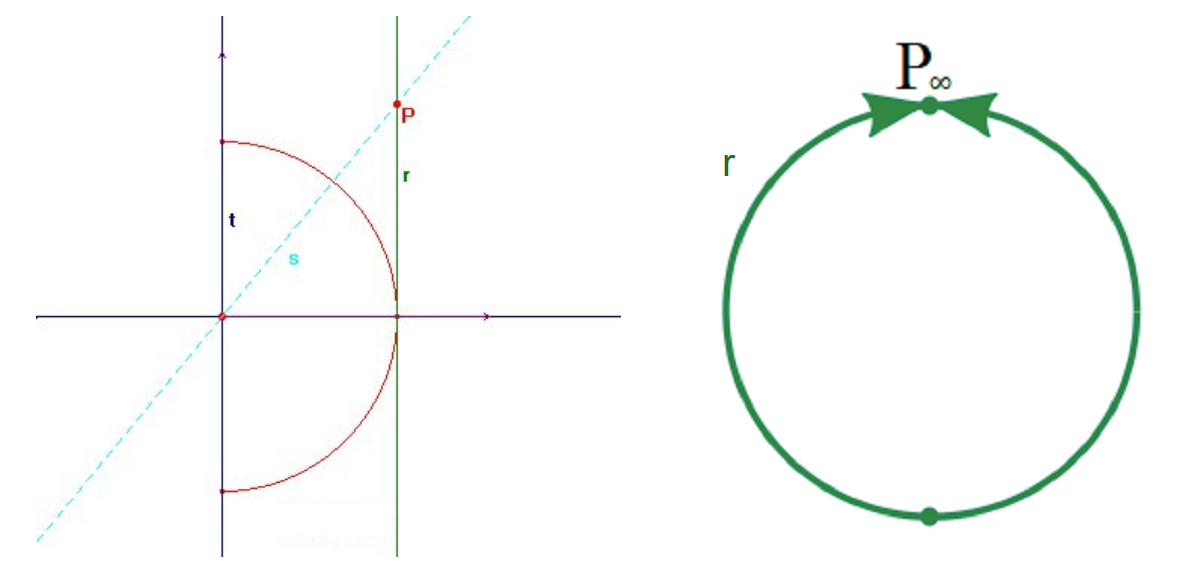
\includegraphics[scale = 0.54]{1.2_1}
\centering
\end{figure}

Se procederá de forma análoga en el caso del plano proyectivo real $\mathcal{P}_2(\R)$, el conjunto de rectas vectoriales de $\R^3$. Se escoge un plano afín $\pi$ que no pase por el origen, por ejemplo el de ecuación $x= 1$. La mayoría de las rectas vectoriales cortan a $\pi$ en un solo punto, que además determina de forma única a cada recta. 

\vspace{2mm}
La excepción ahora es toda recta perteneciente al plano $\pi_\infty$ de ecuación $x = 0$, paralelo a $\pi$. Si $r$ es una de estas rectas y $P_r$ es su punto del infinito, entonces el punto que se adjudica a $\pi$ es $P_r$, ampliándose el plano $\pi$ con los puntos en el infinito de todas las rectas de $\pi_\infty$.

\vspace{2mm}
En resumen, se puede imaginar el plano proyectivo real como un plano afín que no pasa por el origen al que se le añade una recta de puntos en el infinito que rodea a dicho plano.

\begin{figure}[h]
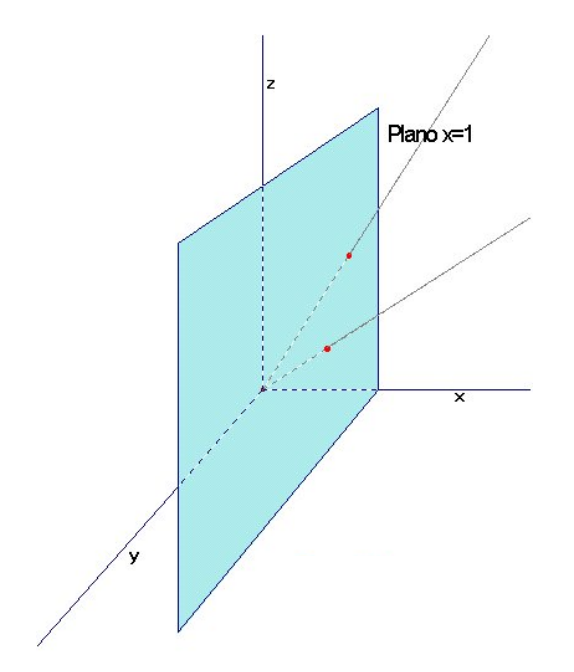
\includegraphics[scale = 0.4]{1.2_2}
\centering
\end{figure}

\section{Coordenadas homogéneas}

Cabe destacar que, a diferencia de lo que ocurría con los puntos de un espacio vectorial, la suma de dos puntos de un espacio proyectivo no siempre es un punto, sino que puede ser una recta: si $P = \ <u>, Q = \ <v>$ con $u,v$ linealmente independientes, entonces la suma de subespacios $P+Q = \mathcal{P}(<u>+<v>) = \mathcal{P}(<u,v>)$ no es un punto. Otros conceptos como la dependencia y la generación sí pueden trasladarse de un espacio vectorial a su espacio proyectivo asociado.

\begin{definition}
Sean $P_1 = \ <u_1>, \mathellipsis, P_n = \ <u_n>$ puntos de un espacio proyectivo $\mathcal{P}(V)$ sobre un cuerpo $\mathbb{K}$. Se dice que estos puntos son \ul{independientes} si los vectores $u_1,\mathellipsis,u_n$ son linealmente independientes.
\end{definition}

Ahora bien, si los puntos de la definición anterior se escriben (de forma equivalente) como $P_1 = \ < \lambda_1 u_1 >, \mathellipsis, P_1 = \ < \lambda_n u_n >$ para ciertos escalares $\lambda_1,\mathellipsis,\lambda_n$, cabría esperar que los puntos sigan siendo independientes (o no independientes). La respuesta la da la siguiente proposición:

\begin{proposition}
Sean $u_1,\mathellipsis,u_n$ vectores del espacio vectorial $V$ sobre el cuerpo $\mathbb{K}$ y sean $\lambda_1,\mathellipsis,\lambda_n \in \mathbb{K}$. Entonces $u_1,\mathellipsis,u_n$ son linealmente independientes si y solo si $\lambda_1 u_1,\mathellipsis, \lambda_n u_n$ son linealmente independientes.
\end{proposition}

\begin{proof}
    Inmediata.
\end{proof}

\begin{definition}
    Sea $S$ un conjunto de puntos del proyectivo $\mathcal{P}(V)$. Al menor subespacio de $\mathcal{P}(V)$ que contiene a $S$ se le denomina \ul{subespacio generado} (o engendrado) por $S$.
\end{definition}

Es claro que si $S =\{P_1,\mathellipsis,P_n\}$, entonces el subespacio generado por $S$ es $P_1 + \mathellipsis + P_n$, y si $P_i = \ <v_i>  \forall \ i = 1,\mathellipsis,n$, entonces $P_1 + \mathellipsis + P_n = \mathcal{P}(<v_1,\mathellipsis,v_n>)$. Además, de las definiciones anteriores se derivan inmediatamente los siguientes resultados:

\begin{itemize}
    \item[(i)] Un solo punto es independiente.
    \item[(ii)] Dos puntos son independientes si y solo si son distintos.
    \item[(iii)] Tres puntos son independientes si y solo si no están en la misma recta. En efecto, si $P = \ <u>, Q = \ <v>, R = \ <w>$, entonces $P$, $Q$ y $R$ son independientes si y solo si $\mathrm{rg}(u,v,w) = 3$. Si fuese $\mathrm{rg}(u,v,w) = 2$, entonces los tres puntos están en la misma recta proyectiva, y si fuese $\mathrm{rg}(u,v,w) = 1$, entonces los tres puntos son iguales, luego también están en una misma recta proyectiva.
    \item[(iv)] Si $\mathrm{dim}(\mathcal{P}(V)) = n$, entonces hay, a lo sumo, $n+1$ puntos independientes. En efecto, si $\mathrm{dim}(\mathcal{P}(V)) = n$, entonces $\mathrm{dim}(V) = n+1$, luego en $V$ hay, a lo sumo, $n+1$ vectores linealmente independientes, y esto significa que no hay más de $n+1$ puntos independientes en $\mathcal{P}(V)$.
    \item[(v)] Si $\mathrm{dim}(\mathcal{P}(V)) = n$ y se toman $n+1$ puntos de $\mathcal{P}(V)$, es lo mismo decir que son independientes que decir que generan el total.
\end{itemize}

En consecuencia, se puede intuir una forma de construir \say{bases de un espacio proyectivo} que quizá permitan asignar unas coordenadas únicas respecto a cada base a todo punto del espacio proyectivo: si $\mathrm{dim}(\mathcal{P}(V)) = n$ y los puntos $P_i = \ <v_i> (i = 0,\mathellipsis,n)$ son independientes, entonces generan el total. Se puede afirmar que $\mathcal{B} = \{v_0,\mathellipsis,v_n\}$ es una base del espacio vectorial $V$, y por tanto, cualquier vector $v \in V$ se escribe de forma única como \[v = x_0 v_0 + \mathellipsis + x_n v_n\] 
lo que provoca la tentación de llamar por coordenadas de un punto $P = \ <v>$ a la tupla $(x_0,\mathellipsis,x_n)$. Ahora bien, si se tomase el vector $\lambda v_0$ como generador de $P_0 = \ <v_0> \ = \ <\lambda v_0>$ para cualquier escalar $\lambda$ no nulo, entonces $P$ tendría como coordenadas $(x_0 \lambda^{-1},x_1,\mathellipsis,x_n)$, que son distintas de las anteriores. Por tanto, no es buena idea tratar de extender el concepto de base de un espacio vectorial a un espacio proyectivo.

\vspace{2mm}
En su lugar, se seguirá usando el concepto de base de un espacio vectorial para dar las coordenadas de un punto de un espacio proyectivo. Sea $\mathcal{B} = \{v_0,\mathellipsis,v_n\}$ una base de $V$. Lo más natural sería decir que las coordenadas del punto $P = \ <v>$ respecto de $\mathcal{B}$ son las coordenadas de $v$ en la misma base, $(x_0,\mathellipsis,x_n)$. Ahora bien, también se puede escribir $P = \ <\lambda v>$ para cualquier escalar $\lambda$ no nulo, lo que daría las coordenadas $(\lambda  x_0,\mathellipsis,\lambda x_n)$ para el mismo punto $P$.

\vspace{2mm}
Para solucionar este problema, se introduce en $\mathbb{K}^{n+1} \setminus \{0,\mathellipsis,0\}$ la siguiente relación de equivalencia:
\[(x_0,\mathellipsis,x_n) \sim (y_0,\mathellipsis,y_n) \iff \exists \ \lambda \in \mathbb{K} \setminus \{0\} \colon y_i = \lambda x_i \ \forall \ i = 0,\mathellipsis,n\]
El motivo por el que se desecha la tupla $(0,\mathellipsis,0)$ es porque el vector $0 = 0v_0+\mathellipsis+0v_n$ no genera ningún punto del espacio proyectivo. Todo esto lleva a lo siguiente:

\begin{definition}
Si $P = \ <v>$ es un punto de $\mathcal{P}(V)$ y $v$ tiene coordenadas $(x_0,\mathellipsis,x_n)$ respecto de cualquier base $\mathcal{B}=\{v_0,\mathellipsis,v_n\}$, se definen las \ul{coordenadas homogéneas} del punto $P$ como la clase de equivalencia en la relación definida anteriormente de la tupla $(x_0,\mathellipsis,x_n)$. A la base $\mathcal{B} = \{v_0,\mathellipsis,v_n\}$ de partida se le denomina \ul{sistema de coordenadas homogéneas}.
\end{definition}

\begin{example}
En $\mathcal{P}_1(\R)$, tomemos la base canónica de $\R^2$, $\mathcal{B} = \{e_1,e_2\}$, y consideremos los puntos $P = \ <(1,1)>$, $P' = \ <(0,2)>$. Entonces las coordenadas homogéneas de $P$ son $P = (1,1) = (2,2) = (\sqrt{5},\sqrt{5})$, y las de $P'$ son $P' = (0,2) = (0,4) = (0,27\sqrt{13})$.
\end{example}

Para fijar un sistema de coordenadas homogéneas no basta con dar los $n+1$ vectores de una base. Esto se debe a que cualquiera de estos vectores se puede multiplicar por un escalar no nulo y se obtiene un sistema de coordenadas homogéneas exactamente igual, en el sentido de que un punto $P$ tiene las mismas coordenadas homogéneas en el primero que en el segundo.

\vspace{2mm}
Se dará a continuación una construcción alternativa de un sistema de coordenadas homogéneas que solucione este ligero inconveniente. Supongamos que $\mathrm{dim}(\mathcal{P}(V)) = n$ (se necesitará que $n \geq 1$) y sean $P_0,\mathellipsis,P_n$ puntos independientes con $P_i = \ <v_i>$ para cada $i = 0,\mathellipsis,n$. Ahora se toma un punto $U = \ <u>$ que no pertenezca a ninguno de los hiperplanos generados por $n$ de entre los $n+1$ puntos independientes. Esto significa que si se escribe
\[u = \lambda_0 v_0 + \mathellipsis + \lambda_n v_n\]
entonces los escalares $\lambda_0, \mathellipsis, \lambda_n$ han de ser todos no nulos. Por ejemplo, si fuese $\lambda_0 = 0$, entonces $u$ estaría en el hiperplano $P_1+\mathellipsis+P_n$. Esto significa que $\{\lambda_0 v_0, \mathellipsis, \lambda_n v_n\}$ es base de $V$, respecto de la cual el vector $u$ tiene coordenadas $(1,\mathellipsis,1)$. 

\vspace{2mm}
El conjunto de los $n+2$ puntos anteriores se representa $\{P_0,\mathellipsis,P_n;U\}$, denominándose \ul{puntos base} a los $n+1$ primeros puntos y \ul{punto unidad} a $U$. Se comprueba fácilmente que este método de obtener un sistema de coordenadas homogéneas no depende de los vectores elegidos como generadores de los puntos.

\vspace{2mm}
En la última definición se dijo que la base $\{P_0,\mathellipsis,P_n\}$ se llama \textit{sistema de cooordenadas homogéneas}. Este término se usará indistintamente para denominar a una tal base de $V$ o al conjunto $\{P_0,\mathellipsis,P_n;U\}$ de puntos base y punto unidad, al que más adelante se le conocerá por un sustantivo diferente.

\begin{example}
En $\mathcal{P}_2(\R)$, sean $P_0 = \ <(1,-1,0)>, P_1 = \ <(1,0,-1)>, P_2 = \ <(0,0,2)>$ y sea $U = \ <(1,-2,7)>$. En primer lugar, como
\[\begin{vmatrix*}[r]
1 & -1 & 0 \\
1 & 0 & -1 \\
0 & 0 & 2
\end{vmatrix*} \neq 0\]
entonces $P_0, P_1, P_2$ son independientes. Además, 
\[\begin{vmatrix*}[r]
1 & -1 & 0 \\
1 & 0 & -1 \\
1 & -2 & 7
\end{vmatrix*} \neq 0 \qquad
\begin{vmatrix*}[r]
1 & 0 & -1 \\
0 & 0 & 2 \\
1 & -2 & 7
\end{vmatrix*} \neq 0 \qquad
\begin{vmatrix*}[r]
1 & -1 & 0 \\
0 & 0 & 2 \\
1 & -2 & 7
\end{vmatrix*} \neq 0\]
luego $U$ no pertenece a $P_0+P_1$, a $P_1+P_2$ ni a $P_0+P_2$. Por tanto, existen escalares $\lambda_1, \lambda_2, \lambda_3$ no nulos tales que
\[(1,-2,7) = \lambda_0(1,-1,0) + \lambda_1(1,0,-1)+\lambda_2(0,0,2)\]
Resolviendo el sistema se obtiene $\lambda_0 = 2,\lambda_1 = -1,\lambda_2 = 3$, por lo que el sistema de coordenadas homogéneas es
\[\{\lambda_0v_0,\lambda_1v_1,\lambda_2v_2\} = \{(2,-2,0),(-1,0,1),(0,0,6)\}\]
ya que, respecto de esta base, el vector $(1,-2,7)$ tiene coordenadas $(1,1,1)$. Ahora calculemos las coordenadas de $P = \ <(-4,4,6)>$ respecto a $\{P_0,P_1,P_2;U\}$:
\[(-4,4,6) = \alpha_0(2,-2,0)+\alpha_1(-1,0,1)+\alpha_2(0,0,6)\]
Al resolver el sistema se obtiene $\alpha_0 = -2, \alpha_1 = 0, \alpha_2 = 1$, así que las coordenadas homogéneas de $P$ son $P = (-2,0,1) = (-1,0,\frac{1}{2})$.
\end{example}

\section{Cambios de base}

Sean $\mathcal{B} = \{v_0,\mathellipsis,v_n\}, \mathcal{B}' = \{v_0',\mathellipsis,v_n'\}$ dos sistemas de coordenadas homogéneas del espacio proyectivo $\mathcal{P}(V)$. La expresión de cada $v'_i$ en función de los $v_i$ es
\[
\begin{cases}
    v_0' = a_{00}v_0+a_{10}v_1+\mathellipsis+a_{n0}v_n \\
    \, \vdots \\
    v_n' = a_{0n}v_0+a_{1n}v_1+\mathellipsis+a_{nn}v_n
\end{cases}
\]
Sea $P = \ <v>$ un punto de $\mathcal{P}(V)$ con coordenadas homogéneas $(x_0',x_1',\mathellipsis,x_n')_{\mathcal{B}'}$. Entonces se tiene que
\[
\begin{aligned}[t]
v &= x_0'v_0'+\mathellipsis+x_n'v_n' \\
&= x_0'(a_{00}v_0+a_{10}v_1+\mathellipsis+a_{n0}v_n)+\mathellipsis+x_n'(a_{0n}v_0+a_{1n}v_1+\mathellipsis+a_{nn}v_n) \\
&= (a_{00}x_0'+\mathellipsis+a_{0n}x_n')v_0+(a_{10}x_0'+\mathellipsis+a_{1n}x_n')v_1+\mathellipsis+(a_{n0}x_0'+\mathellipsis+a_{nn}x_n')v_n
\end{aligned}
\]
Si se llama $x_i = a_{i0}x_0'+\mathellipsis+a_{in}x_n'$, entonces las coordenadas homogéneas de $P$ en el sistema de referencia $\mathcal{B}$ son $(x_0,x_1,\mathellipsis,x_n)_{\mathcal{B}}$. Lo anterior suele escribirse en forma matricial como
\[\begin{pmatrix*}
    a_{00} & a_{01} & \mathellipsis & a_{0n} \\
    a_{10} & a_{11} & \mathellipsis & a_{1n} \\
    \vdots & \vdots & \ddots & \vdots \\
    a_{n0} & a_{n1} & \mathellipsis & a_{nn}
\end{pmatrix*}
\begin{pmatrix*}
    x_0' \\
    x_1' \\
    \vdots \\
    x_n'
\end{pmatrix*} = \lambda \begin{pmatrix*}
    x_0 \\
    x_1 \\
    \vdots \\
    x_n
\end{pmatrix*} \iff
AX' = \lambda X
\]
donde el escalar no nulo $\lambda$ se escribe para indicar que se trata de coordenadas homogéneas. La expresión $AX' = \lambda X$ se denomina \ul{ecuación del cambio de coordenadas homogéneas} de $\mathcal{B'}$ a $\mathcal{B}$. Como $A$ es la matriz de un cambio de base, entonces posee inversa:
\[A^{-1} = \frac{1}{\mathrm{det}(A)} \, \mathrm{adj}(A^t)\]
El cambio de base (vectorial) recíproco sería
\[X' = A^{-1}X = \frac{1}{\mathrm{det}(A)} \, \mathrm{adj}(A^t) \, X\]
En el caso proyectivo, como $\frac{1}{\mathrm{det}(A)}$ es un escalar cualquiera, se puede escribir
\[X' = \lambda \, \mathrm{adj}(A^t) \, X\]

\begin{example}
En el plano proyectivo $\mathcal{P}_2(\R)$, tomemos el sistema de coordenadas homogéneas dado por $P_0 = \ <(-1,1,2)>, P_1 = \ <(1,-1,0)>, P_2 = \ <(1,0,1)>$ y $ U = \ <(2,1,-1)>$ (se comprueba que los $P_i$ son independientes y que $U$ no pertenece a ninguno de los hiperplanos generados por cualquier par de los tres puntos base). Se denotará por $SCH_B$ al sistema de coordenadas homogéneas $\{(2,-2,0),(-1,0,1),(0,0,6)\}$ (el del ejemplo anterior) y por $SCH_A$ al otro. Se trata de calcular $SCH_A$, dar las coordenadas de $P = \ <(2,1,-3)>$ en $SCH_A$ y calcular el cambio de base de $SCH_B$ a $SCH_A$. Se tiene que
\[(2,1,-1) = \lambda_0(-1,1,2)+\lambda_1(1,-1,0)+\lambda_2(1,0,1)\]
y resolviendo el sistema correspondiente se obtiene $\lambda_0 = -2, \lambda_1 = -3, \lambda_2 = 3$. Por tanto, el sistema $SCH_A$ sería $\{(2,-2,-4),(-3,3,0),(3,0,3)\}$. El sistema de ecuaciones dado por
\[(2,1,-3) = \alpha_0(2,-2,-4)+\alpha_1(-3,3,0)+\alpha_2(3,0,3)\]
tiene como solución $\alpha_0 = \frac{3}{2}, \alpha_1 = \frac{4}{3}, \alpha_2 = 1$, así que $P$ tiene coordenadas homogéneas $P = (\frac{3}{2},\frac{4}{3},1) = (9,8,6)$ respecto a $SCH_A$. Escribiendo los vectores de $SCH_B$ en función de $SCH_A$, se tienen las ecuaciones
\[
\begin{aligned}[t]
(2,-2,0) &= a_{00}(2,-2,-4)+a_{01}(-3,3,0)+a_{02}(3,0,3) \\
(-1,0,1) &= a_{10}(2,-2,-4)+a_{11}(-3,3,0)+a_{12}(3,0,3) \\
(0,0,6) &= a_{20}(2,-2,-4)+a_{21}(-3,3,0)+a_{22}(3,0,3)  
\end{aligned}
\]

cuya resolución da los coeficientes de la matriz del cambio de base:
\[A = \begin{pmatrix*}
0 & 1/2 & 3/2 \\
 2/3 &  1/3 & 1 \\
0 & 1/3 & 0
\end{pmatrix*} = \begin{pmatrix*}[r]
0 & 3 & 9 \\
4 & 2 & 6 \\
0 & 2 & 0
\end{pmatrix*}\]
Nótese que el significado del último símbolo $=$ es la igualdad de ambas matrices como matrices del cambio de coordenadas homogéneas. Así, si un punto $P$ tiene coordenadas $P = (x_0',x_1',x_2')$ respecto de $SCH_B$, entonces la ecuación del cambio sería
\[\begin{pmatrix*}[r] 
0 & 3 & 9 \\
4 & 2 & 6 \\
0 & 2 & 0
\end{pmatrix*} \begin{pmatrix*}[r]
x_0' \\
x_1' \\
x_2'
\end{pmatrix*}_{\!\!B} = \lambda \begin{pmatrix*}[r]
x_0 \\
x_1 \\
x_2
\end{pmatrix*}_{\!\!A}\]
\end{example}

\section{Determinación de subespacios por sus ecuaciones}
De la misma forma que un punto queda caracterizado por sus coordenadas, los subespacios proyectivos quedarán determinados por un conjunto de puntos cuyas coordenadas satisfagan ciertas relaciones.

\vspace{2mm}
Sean $P_i = \ <u_i>$, $i \in \{0,1,\mathellipsis,k\}$ puntos independientes de un espacio proyectivo $\mathcal{P}(V)$ de dimensión $n$ ($k \leq n$) sobre el cuerpo $\mathbb{K}$ y sea $\{v_0,v_1,\mathellipsis,v_n\}$ un sistema de coordenadas homogéneas. El subespacio proyectivo $\mathcal{S} = P_0+P_1+\mathellipsis+P_k$ tiene dimensión $k$. Si $<u>$ es un punto de $\mathcal{P}(V)$, entonces
\[<u> \, \in \mathcal{S} \iff
\begin{aligned}[t]
\exists \ \lambda_0,\mathellipsis,\lambda_k \in \mathbb{K} \colon u &= \lambda_0u_0+\mathellipsis+\lambda_ku_k \\
&= (\lambda_0a_{00}+\mathellipsis+\lambda_ka_{k0},\mathellipsis,\lambda_0a_{0n}+\mathellipsis+\lambda_ka_{kn})_{\mathcal{B}}
\end{aligned}
\]
donde $u_i = a_{i0}v_0+\mathellipsis+a_{in}v_n$ para cada $i \in \{0,1,\mathellipsis,k\}$. Por tanto, variando los escalares $\lambda_0,\mathellipsis,\lambda_k$ se obtienen todos los posibles puntos del subespacio $\mathcal{S}$, lo que se expresa mediante las ecuaciones
\[
\begin{cases}
    \lambda x_0 = \lambda_0a_{00}+\mathellipsis+\lambda_ka_{k0} \\
    \lambda x_1 = \lambda_0a_{01}+\mathellipsis+\lambda_ka_{k1} \\
    \ \, \vdots \\
    \lambda x_n = \lambda_0a_{0n}+\mathellipsis+\lambda_ka_{kn}
\end{cases}
\]
las cuales se denominan \ul{ecuaciones paramétricas} de $\mathcal{S}$. De forma similar al caso de los subespacios vectoriales, los $x_i$ constituyen las coordenadas homogéneas de cada punto de $\mathcal{S}$, que una vez se pueden dar multiplicadas por cualquier escalar $\lambda$ no nulo.

\vspace{2mm}
La obtención de las ecuaciones cartesianas de un subespacio proyectivo también será análoga a aquella de los subespacios vectoriales. La matriz
\[A = \begin{pmatrix*}
    a_{00} & \mathellipsis & a_{0n} \\
    \vdots & \ddots & \vdots \\
    a_{k0} & \mathellipsis & a_{kn} \\
    x_0 & \mathellipsis & x_n
\end{pmatrix*}\]
es de rango $k+1$ si y solo si el punto de coordenadas homogéneas $(x_0,\mathellipsis,x_n)$ pertenece a $\mathcal{S}$, lo que proporciona $n-k$ ecuaciones a las que se les llama \ul{ecuaciones cartesianas} de $\mathcal{S}$. Si $\mathcal{P}(S)$ es un subespacio de dimensión $k$ de $\mathcal{P}(V)$, que tiene dimensión $n$, entonces las ecuaciones paramétricas de $\mathcal{P}(S)$ tienen $k+1$ parámetros y las cartesianas tienen $n-k$ ecuaciones.

\begin{example}
En $\mathcal{P}_2(\R)$, tomemos la base $\mathcal{B} = \{(2,-2,0),(-1,0,1),(0,0,6)\}$ y los puntos $P_0 = \ < u_0 >$, $P_1 = \ < u_1>$, donde $u_0 = (1,0,1)$ y $u_2 = (0,1,1)$. Hallemos las ecuaciones paramétricas de $\mathcal{P}(S) = P_0+P_1$. Resolviendo el sistema dado por las ecuaciones
\[(1,0,1) = \alpha(2,-2,0)+\beta(-1,0,1)+\gamma(0,0,6)\]
\[(0,1,1) = \alpha'(2,-2,0)+\beta'(-1,0,1)+\gamma'(0,0,6)\]
se obtiene $u_0 = (0,-1,\frac{1}{3})_{\mathcal{B}}$, $u_1 = (-\frac{1}{2},-1,\frac{1}{3})_{\mathcal{B}}$. Las paramétricas de $\mathcal{P}(S)$ serían
\[
\begin{pmatrix*}[r]
\lambda x_0 \\
\lambda x_1 \\
\lambda x_2
\end{pmatrix*} = \lambda_0 \begin{pmatrix*}[r]
0 \\
-1 \\
\frac{1}{3}
\end{pmatrix*}
+ \lambda_1 \begin{pmatrix*}[r]
-\frac{1}{2} \\
-1 \\
\frac{1}{3}
\end{pmatrix*} = \lambda_0 \begin{pmatrix*}[r]
0 \\
-3 \\
1
\end{pmatrix*}
+ \lambda_1 \begin{pmatrix*}[r]
3 \\
6 \\
-2
\end{pmatrix*}
\]
\end{example}

\section{El espacio afín dentro del proyectivo}

\begin{definition}
\label{def1.9.}
Sea $V$ un espacio vectorial sobre el cuerpo $\mathbb{K}$ y sea $H$ un hiperplano de $V$. El conjunto 
\[\mathcal{A}(V,H) = \mathcal{P}(V) \setminus \mathcal{P}(H)\]
se dice que es un \ul{espacio afín} sobre $\mathbb{K}$. De $\mathcal{P}(V)$ se dirá que es la \ul{envolvente proyectiva} de $\mathcal{A}(V,H)$. A los puntos de $\mathcal{P}(H)$ se les llama \ul{puntos del infinito} o \ul{puntos impropios} y a $\mathcal{P}(H)$, \ul{hiperplano del infinito} o \ul{hiperplano impropio}. La \ul{dimensión} del espacio afín $\mathcal{A}(V,H)$ es la que tuviera el espacio proyectivo $\mathcal{P}(V)$.
\end{definition}

Recuérdese que la recta proyectiva real no es más que una recta afín que no pasa por el origen y a la que se le añade un punto en el infinito. Si se elimina de esta recta el punto del infinito (un hiperplano de la recta proyectiva), lo que resta no es más que una recta afín normal y corriente, lo que le da sentido a esta definición de espacio afín y a la denominación de \textit{hiperplano del infinito}. En el plano proyectivo real, tres cuartos de lo mismo.

\begin{definition}
Un subconjunto $T$ del espacio afín $\mathcal{A}(V,H)$ se dice que es un \ul{subespacio afín} si existe un subespacio vectorial $U$ de $V$ tal que $U \not\subset H$ y $T = \mathcal{P}(U) \setminus \mathcal{P}(H)$.
\end{definition}

\begin{proposition}
\label{prop1.3.}
Sea $\mathcal{P}(V)$ un espacio proyectivo de dimensión $n$ y sea $\mathcal{P}(H)$ un hiperplano de $\mathcal{P}(V)$ engendrado por los puntos $P_i = \ <v_i>, \, i = 1,\mathellipsis,n$.
\begin{itemize}
    \item[(i)] Si $P_0 = \ <v_0>$ es un punto de $\mathcal{A}(V,H)$, entonces $\{v_0,v_1,\mathellipsis,v_n\}$ es un sistema de coordenadas homogéneas de $\mathcal{P}(V)$.
    \item[(ii)] La única ecuación cartesiana de $\mathcal{P}(H)$ es $x_0 = 0$.
    \item[(iii)] $P = (x_0,\mathellipsis,x_n) \in \mathcal{A}(V,H)$ si y solo si $x_0 \neq 0$.
\end{itemize}
\end{proposition}

\begin{proof}
\hfill
    \begin{itemize}
        \item[(i)] Como los puntos $\, <v_0>, \, <v_1>,\mathellipsis, \, <v_n> \ $ son independientes, entonces el conjunto de vectores $\{v_0,v_1,\mathellipsis,v_n\}$ forma una base de $V$, o lo que es lo mismo, es un sistema de coordenadas homogéneas de $\mathcal{P}(V)$.
        \item[(ii)] Sea $P = \ <u>$ un punto de coordenadas homogéneas $(x_0,x_1,\mathellipsis,x_n)$ en el sistema de coordenadas homogéneas del apartado anterior, es decir, $u = x_0v_0+x_1v_1+\mathellipsis+x_nv_n$. Como $\mathcal{P}(H) = P_1+\mathellipsis+P_n$, entonces $P \in \mathcal{P}(H)$ si y solo si $x_0 = 0$.
        \item[(iii)] Consecuencia inmediata del apartado anterior.
    \end{itemize}
\end{proof}

\begin{theorem}
\label{teo1.1.}
Sea $\mathcal{P}(H)$ un hiperplano del espacio proyectivo de dimensión $n$ $\mathcal{P}(V)$ sobre el cuerpo $\mathbb{K}$. Entonces existe una biyección entre $\mathcal{A}(V,H)$ y $\mathbb{K}^n$. Explícitamente,
\[
\begin{aligned}[t]
    \mathcal{A}(V,H) &\longrightarrow \mathbb{K}^n \\
    (x_0,x_1,\mathellipsis,x_n) &\longmapsto \biggl(\frac{x_1}{x_0},\frac{x_2}{x_0},\mathellipsis,\frac{x_n}{x_0}\biggr)
\end{aligned}
\]
\end{theorem}

\begin{proof}
En primer lugar, la aplicación está bien definida, pues el punto de coordenadas homogéneas $(x_0,x_1,\mathellipsis,x_n)$ pertenece a $\mathcal{A}(V,H)$ si y solo si $x_0 \neq 0$. Además, si $(x_0',x_1',\mathellipsis,x_n')$ es otro representante de las mismas coordenadas homogéneas entonces existe $\lambda \in \mathbb{K} \setminus \{0\}$ tal que $x_i' = \lambda x_i \ \forall \ i = 0,1,\mathellipsis,n$. Por tanto,
\[(x_0',x_1',\mathellipsis,x_n') = (\lambda x_0, \lambda x_1,\mathellipsis, \lambda x_n) \longmapsto \biggl(\frac{\lambda x_1}{\lambda x_0}, \frac{\lambda x_2}{\lambda x_0}, \mathellipsis, \frac{\lambda x_n}{\lambda x_0}\biggr) = \biggl(\frac{x_1}{x_0}, \frac{x_2}{x_0}, \mathellipsis, \frac{x_n}{x_0}\biggr)\]
Se comprueba fácilmente que la aplicación así definida tiene como inversa a
\[
\begin{aligned}[t]
    \mathbb{K}^n &\longrightarrow \mathcal{A}(V,H) \\
    (y_1,\mathellipsis,y_n) &\longmapsto (1,y_1,\mathellipsis,y_n)
\end{aligned}
\]
de donde se deduce el carácter biyectivo de dicha aplicación.
\end{proof}

\begin{definition}
Dado un punto $P = (x_0,x_1,\mathellipsis,x_n)$ del espacio afín $\mathcal{A}(V,H)$, los elementos de la tupla $(\frac{x_1}{x_0},\frac{x_2}{x_0},\mathellipsis,\frac{x_n}{x_0})$ se dice que son las \ul{coordenadas cartesianas} de $P$.
\end{definition}
Por último, cabe remarcar que la posición del $1$ al pasar de coordenadas cartesianas a homogéneas depende del orden en que se tomen los vectores del sistema de coordenadas homogéneas de $\mathcal{P}(V)$. Por ejemplo, si en (i) de la \hyperref[prop1.3.]{\color{blue}Proposición 1.4} se tomase el sistema $\{v_1,\mathellipsis,v_n,v_0\}$ entonces la biyección entre $\mathcal{A}(V,H)$ y $\mathbb{K}^n$ y su inversa serían
\begin{equation*}
\begin{aligned}[t]
    \mathcal{A}(V,H) &\longrightarrow \mathbb{K}^n \\
    (x_1,\mathellipsis,x_n,x_0) &\longmapsto \biggl(\frac{x_1}{x_0},\frac{x_2}{x_0},\mathellipsis,\frac{x_n}{x_0}\biggr)
\end{aligned}
\qquad
\begin{aligned}[t]
    \mathbb{K}^n &\longrightarrow \mathcal{A}(V,H) \\
    (y_1,\mathellipsis,y_n) &\longmapsto (y_1,\mathellipsis,y_n,1)
\end{aligned}
\end{equation*}

\begin{example}
Tomemos $V = \R^3$, $H = \ <e_1,e_2>$ y $S = \ <e_2,e_3>$ ($\mathcal{B} = \{e_1,e_2,e_3\}$ es la base canónica). Un $P \in \mathcal{P}_2(\R)$ con coordenadas homogéneas $(x_0,x_1,x_2)$ está en $\mathcal{P}(H)$ si y solo si $x_2 = 0$, y está en $\mathcal{P}(S)$ si y solo si $x_0 = 0$. Por tanto, el subespacio afín $T = \mathcal{P}(S) \setminus \mathcal{P}(H)$ es
\[T = \{(x_0,x_1,x_2) \colon x_0 = 0, x_2 \neq 0\}\]
\end{example}

\section{Principio de dualidad}
Como se vio en el tema anterior, entre la familia de subespacios de un espacio vectorial $V$ de dimensión $n$ y la familia de subespacios del espacio dual $V^*$ se establecen dos aplicaciones 
\begin{equation*}
\begin{aligned}[t]
\varphi \colon S(V) &\longrightarrow S(V^*) \\
U &\longmapsto \varphi(U) = V^\circ
\end{aligned}
\qquad
\begin{aligned}[t]
\varphi^{-1} \colon S(V^*) &\longrightarrow S(V) \\
W &\longmapsto \varphi^{-1}(W) = W^\circ
\end{aligned}
\end{equation*}
que resultan ser antiisomorfismos de retículos, es decir, son isomorfismos de retículos que invierten inclusiones y que transforman sumas en intersecciones e intersecciones en sumas:
\[U \subset W \implies W^\circ \subset U^\circ \qquad (U+W)^\circ = U^\circ \cap W^\circ \qquad (U \cap W)^\circ = U^\circ + W^\circ\]

A cualquiera de estas dos aplicaciones se le denomina \ul{correlación estándar}. Por otro lado, si $S \in S(V)$ es un subespacio de $V$ de dimensión $k$, entonces $S^* \in S(V^*)$ es un subespacio de $V^*$ de dimensión $n-k$ (y viceversa). De esto se deduce...
\begin{theorem}[Principio de dualidad]
Todo teorema en espacios proyectivos de dimensión $n$ sobre $\mathbb{K}$, enunciado en términos de inclusiones, sumas y/o intersecciones de subespacios, proporciona un teorema dual, igualmente válido en espacios proyectivos de dimensión $n$ sobre el mismo cuerpo, obtenido mediante la inversión de las inclusiones, la sustitución de las sumas por intersecciones, de las intersecciones por sumas, y los subespacios de dimensión $r$ por subespacios de dimensión $n-r-1$.
\end{theorem}

Respecto a esta última línea, si $\mathrm{dim}(\mathcal{P}(V)) =n$, entonces $\mathrm{dim}(V) = n+1$, así que si $\mathrm{dim}(\mathcal{P}(S)) = r$, entonces $\mathrm{dim}(\mathcal{P}(S^*)) = \mathrm{dim}(S^*)-1 = \mathrm{dim}(V) - \mathrm{dim}(S) - 1 = n-r-1$. En resumen, dado un espacio vectorial $V$ sobre el cuerpo $\mathbb{K}$, se tienen las correspondencias

\begin{align*}
\Aboxed{\mathcal{P}(V) &\longleftrightarrow \mathcal{P}(V^*)} \\[5pt]
H \equiv \Bigl\{a_0x_0+\mathellipsis a_nx_n = 0 &\longleftrightarrow P = (a_0,\mathellipsis,a_n) \\[5pt]
\mathcal{P}(S) \subset \mathcal{P}(T) &\longleftrightarrow \mathcal{P}(T^\circ) \subset \mathcal{P}(S^\circ)\\[10pt]
\mathcal{P}(S \cap T) = \mathcal{P}(S) \cap \mathcal{P}(T) &\longleftrightarrow \mathcal{P}(S^\circ + T^\circ) = \mathcal{P}(S^\circ)+\mathcal{P}(T^\circ) \\[10pt]
\mathcal{P}(S + T) = \mathcal{P}(S) + \mathcal{P}(T) &\longleftrightarrow \mathcal{P}(S^\circ \cap T^\circ) = \mathcal{P}(S^\circ) \cap \mathcal{P}(T^\circ) \\[10pt]
\mathrm{dim}(\mathcal{P}(S)) = k &\longleftrightarrow \mathrm{dim}(\mathcal{P}(S^\circ)) = n-k-1 \\
\end{align*}
\normalsize
\begin{example}
En el plano proyectivo, el término dual de punto es recta, y el de recta, punto. Además,
\begin{multicols}{2}
\noindent \textbf{Definición}. Dos puntos $P,Q$ se dice que están \ul{alineados} si su suma (que se denota $\overline{PQ}$) es una recta.

\columnbreak

\noindent \textbf{Definición dual}. Dos rectas $r,s$ se dice que son \ul{concurrentes} si su intersección es un punto.
\end{multicols}

\begin{multicols}{2}
\noindent \textbf{Teorema}. Una recta $r$ está determinada por dos puntos independientes $A$ y $B$, es decir, $r = \overline{AB} = A+B$.

\columnbreak

\noindent \textbf{Teorema dual}. Un punto $P$ está determinado por la intersección de dos rectas $r$ y $s$ distintas, es decir, $P = r \cap s$.
\end{multicols}
\end{example}

\begin{example}
En espacios proyectivos tridimensionales, los duales de los planos son los puntos (y viceversa) y las rectas son términos duales de sí mismas. Además,
\begin{multicols}{2}
\noindent \textbf{Teorema}. Tres puntos no alineados generan un único plano $\pi = P + Q + R$.

\columnbreak

\noindent \textbf{Teorema dual}. Tres planos $\pi_1,\pi_2,\pi_3$ sin rectas comunes se cortan en un único punto $P = \pi_1 \cap \pi_2 \cap \pi_3$.
\end{multicols}
\end{example}

\chapter{Proyectividades e involuciones}

\section{Proyectividades}

De la misma forma que entre espacios vectoriales se definían aplicaciones lineales, el primer objetivo de este tema será definir aplicaciones entre espacios proyectivos.

\vspace{2mm}
Sean $V,V'$ espacios vectoriales sobre el cuerpo $\mathbb{K}$ y sea $f \colon V \to V'$ una aplicación lineal. Dado un punto $P = \ <v>$ del espacio proyectivo $\mathcal{P}(V)$, aparece la tentación de definir una aplicación $\mathcal{P}(f) \colon \mathcal{P}(V) \to \mathcal{P}(V')$ por $\mathcal{P}(f)(P) = \ <f(v)>$. Esta idea, por muy natural que sea, presenta el inconveniente de que $f(v)$ pudiera ser nulo y por tanto $<f(v)>$ no sería un punto de $\mathcal{P}(V')$. Este impedimento es de fácil solución: pedir que $\mathrm{Ker}(f) = \{0\}$, o lo que es lo mismo, que $f$ sea inyectiva.

\begin{proposition}
Si $f \colon V \to V'$ es una aplicación lineal inyectiva, entonces la aplicación
\[
\begin{aligned}[t]
\mathcal{P}(f) \colon \mathcal{P}(V) &\longrightarrow \mathcal{P}(V') \\
P = \ <v> \, &\longmapsto \mathcal{P}(f)(P) = \ <f(v)>
\end{aligned}
\]
está bien definida y verifica 
\[\mathcal{P}(id_V) = id_{\mathcal{P}(V)} \qquad \mathcal{P}(f \circ g) = \mathcal{P}(f) \circ \mathcal{P}(g)\]
\end{proposition}

\begin{proof}
    Ejercicio.
\end{proof}

\begin{definition}
La aplicación $\mathcal{P}(f)$ definida en la proposición anterior se llamará \ul{aplicación inducida por $f$}. Cuando $f$ sea un isomorfismo, se dirá que $\mathcal{P}(f)$ es una \ul{proyectividad}.
\end{definition}

\begin{definition}
    Una aplicación $f \colon V \to V'$ lineal e inyectiva se denomina \ul{transformación regular}.
\end{definition}

\begin{proposition}
Sean $\mathcal{P}(V)$, $\mathcal{P}(V')$ espacios proyectivos sobre el cuerpo $\mathbb{K}$.
    \begin{itemize}
        \item[(i)] Si $\mathcal{P}(f) \colon \mathcal{P}(V) \to \mathcal{P}(V')$ es la aplicación inducida por una transformación regular $f$, entonces $\mathrm{dim}(\mathcal{P}(V)) \leq \mathrm{dim}(\mathcal{P}(V'))$.
        \item[(ii)] $\sigma \colon \mathcal{P}(V) \to \mathcal{P}(V')$ es una proyectividad si y solo si $\mathrm{dim}(\mathcal{P}(V)) = \mathrm{dim}(\mathcal{P}(V'))$.
        \item[(iii)] Si $\sigma \colon \mathcal{P}(V) \to \mathcal{P}(V')$ es una proyectividad  y $\mathcal{P}(S)$ es un subespacio de $\mathcal{P}(V)$, entonces $\sigma(\mathcal{P}(S))$ es un subespacio proyectivo de $\mathcal{P}(V')$ y $\mathrm{dim}(\mathcal{P}(S)) = \mathrm{dim}(\sigma(\mathcal{P}(S)))$.
        \item[(iv)] La inversa de una proyectividad es una proyectividad.
        \item[(v)] Una proyectividad $\mathcal{P}(f) \colon \mathcal{P}(V) \to \mathcal{P}(V')$ induce un isomorfismo de retículos dado por 
        \[
        \begin{aligned}[t]
        S(\mathcal{P}(V)) &\longrightarrow  S(\mathcal{P}(V')) \\
        \mathcal{P}(T) &\longmapsto \mathcal{P}(f)(\mathcal{P}(T)) = \mathcal{P}(f(T))
        \end{aligned}
        \]
        es decir, $\mathcal{P}(f)$ conserva las inclusiones, sumas e intersecciones de subespacios.
        \item[(vi)] Una proyectividad $\sigma \colon \mathcal{P}(V) \to \mathcal{P}(V')$ aplica puntos alineados en puntos alineados, es decir, si $A \in \overline{BC}$, entonces $\sigma(A) \in \overline{\sigma(B)\sigma(C)}$.
    \end{itemize}
\end{proposition}

\begin{proof}
Es inmediata recordando que
\begin{itemize}
    \item[(i)] Toda transformación regular envía vectores linealmente independientes en vectores linealmente independientes.
    \item[(ii)]$V \cong V'$ si y solo si $\mathrm{dim}(V) = \mathrm{dim}(V')$.
    \item[(iii)] Toda aplicación lineal transforma subespacios en subespacios y conserva dimensiones.
    \item[(iv)] La inversa de un isomorfismo es también isomorfismo.
\end{itemize}
La demostración de (v) y (vi) es una simple comprobación.
\end{proof}

A continuación, se tratará de dar la ecuación de una proyectividad. Considérese una proyectividad $\mathcal{P}(f) \colon \mathcal{P}(V) \to \mathcal{P}(V')$ entre espacios proyectivos de dimensión $n$ y sean $\mathcal{B}$ y $\mathcal{B'}$ sistemas de coordenadas homogéneas de $\mathcal{P}(V)$ y $\mathcal{P}(V')$, respectivamente. La matriz de la aplicación lineal $f$ respecto de las bases $\mathcal{B}$ y $\mathcal{B'}$ es
\[A = \mathcal{M}_{\mathcal{B},\mathcal{B'}}(f) = \begin{pmatrix*}
    a_{11} & a_{21} & \mathellipsis & a_{n1} \\
    a_{12} & a_{22} & \mathellipsis & a_{n2} \\
    \vdots & \vdots & \ddots & \vdots \\
    a_{1n} & a_{2n} & \mathellipsis & a_{nn}
\end{pmatrix*}\]
Si un punto $P \in \mathcal{P}(V)$ tiene coordenadas homogéneas $(x_1,x_2,\mathellipsis,x_n)_{\mathcal{B}}$ y su imagen $\mathcal{P}(f)(P)$ tiene coordenadas homogéneas $(x'_1,x'_2,\mathellipsis,x'_n)_{\mathcal{B'}}$, entonces la relación entre las coordenadas viene dada por
\[Ax = \lambda x' \iff \begin{pmatrix*}
    a_{11} & a_{21} & \mathellipsis & a_{n1} \\
    a_{12} & a_{22} & \mathellipsis & a_{n2} \\
    \vdots & \vdots & \ddots & \vdots \\
    a_{1n} & a_{2n} & \mathellipsis & a_{nn}
\end{pmatrix*} \begin{pmatrix*}
    x_1 \\
    x_2 \\
    \vdots \\
    x_n
\end{pmatrix*} = \lambda \begin{pmatrix*}
    x'_1 \\
    x'_2 \\
    \vdots \\
    x'_n
\end{pmatrix*}\]

Esta ecuación no es más que la ecuación de una aplicación lineal pero con la precaución de multiplicar por un escalar las coordenadas de la imagen por estar trabajando con coordenadas homogéneas.

\begin{example}
Considérese la aplicación lineal $f \colon \R^3 \to \R^3$ definida por
\[f(x_0,x_1,x_2) = (2x_0-x_1,x_0+x_1+x_2,-x_1-x_2)\]
y el sistema de coordenadas homogéneas canónico tanto en el dominio como en la imagen. Se comprueba que $f$ es isomorfismo, por lo que la aplicación $\mathcal{P}(f)$ que induce es una proyectividad. Se tiene que
\[
\begin{aligned}[t]
    P_0 = \ <(1,0,0)> \, &\longmapsto \mathcal{P}(f)(P_0) = \ <(2,1,0)> \\
    P_1 = \ <(0,1,0)> \, &\longmapsto \mathcal{P}(f)(P_1) = \ <(-1,1,-1)> \\
    P_2 = \ <(0,0,1)> \, &\longmapsto \mathcal{P}(f)(P_2) = \ <(0,1,-1)> \\
    U = \ <(1,1,1)> \, &\longmapsto \mathcal{P}(f)(U) = \ <(1,3,-2)> \\
\end{aligned}
\]
así que la ecuación de la proyectividad sería
\[\begin{pmatrix*}[r]
    2 & -1 & 0 \\
    1 & 1 &  1 \\
    0 & -1 & -1
\end{pmatrix*} \begin{pmatrix*}[r]
    x_1 \\
    x_2 \\
    x_3
\end{pmatrix*} = \lambda \begin{pmatrix*}[r]
    x'_1 \\
    x'_2 \\
    x'_3
\end{pmatrix*}\]
Cabe remarcar que esta ecuación depende de las bases elegidas. Si para cada $i =1,2,3$ se llama $Q_i = \mathcal{P}(f)(P_i)$ y $V = \mathcal{P}(f)(U)$, por ser $f$ biyectiva se tiene que $\{Q_1,Q_2,Q_3;V\}$ es un sistema de coordenadas homogéneas de $\mathcal{P}_2(\R)$. Considerando este sistema en la imagen y manteniendo el canónico en el dominio, la ecuación de la proyectividad sería ahora
\[\begin{pmatrix*}[r]
    1 & 0 & 0 \\
    0 & 1 & 0 \\
    0 & 0 & 1
\end{pmatrix*} \begin{pmatrix*}[r]
    x_1 \\
    x_2 \\
    x_3
\end{pmatrix*} = \lambda \begin{pmatrix*}[r]
    x'_1 \\
    x'_2 \\
    x'_3
\end{pmatrix*} \iff \begin{pmatrix*}[r]
    x_1 \\
    x_2 \\
    x_3
\end{pmatrix*} = \lambda \begin{pmatrix*}[r]
    x'_1 \\
    x'_2 \\
    x'_3
\end{pmatrix*}\]
\end{example}

\section{Afinidades}
Se trata ahora de definir aplicaciones entre espacios afines. Sea $f \colon V \to V'$ un isomorfismo entre espacios vectoriales de dimensión $n+1$. Todo hiperplano $H$ de $V$ es enviado por $f$ al hiperplano $f(H) = H'$ de $V'$. Como $\mathcal{P}(f)(\mathcal{P}(H)) = \mathcal{P}(f(H)) = \mathcal{P}(H')$, al restringir el dominio de la proyectividad $\mathcal{P}(f)$ al espacio afín $\mathcal{A}(V,H)$, la imagen se restringirá a $\mathcal{A}(V',H')$. De aquí sale la siguiente definición:

\begin{definition}
La restricción $\bigl.\mathcal{P}(f)\bigr|_{\mathcal{A}(V,H)} = \mathcal{A}(f) \colon \mathcal{A}(V,H) \to \mathcal{A}(V',H')$ descrita en el párrafo anterior se denomina \ul{afinidad}.
\end{definition}

Ahora se dará la ecuación de una afinidad. Fijado un hiperplano $H$ de $V$ y una afinidad $\mathcal{A}(f)$, se consideran sistemas de coordenadas homogéneas $\mathcal{B} = \{u_0,u_1,\mathellipsis,u_n\}$ de $\mathcal{P}(V)$ y $\mathcal{B'} = \{v_0,v_1,\mathellipsis,v_n\}$ de $\mathcal{P}(V')$ tales que
\[H = \ <u_1,\mathellipsis,u_n> \qquad H' = \ <v_1,\mathellipsis,v_n>\]
Expresando la imagen de la base $\mathcal{B}$ respecto de $\mathcal{B'}$,
\[\begin{cases}
    f(u_0) = a_{00}v_0+a_{10}v_1+\mathellipsis+a_{n0}v_n\\
    f(u_1) = a_{01}v_0+a_{11}v_1+\mathellipsis+a_{n1}v_n\\
    \ \ \ \vdots \\
    f(u_n) = a_{0n}v_0+a_{1n}v_1+\mathellipsis+a_{nn}v_n
\end{cases}\]
La ecuación de la proyectividad $\mathcal{P}(f)$ sería
\[
\begin{pmatrix*}
    a_{00} & a_{01} & \mathellipsis & a_{0n} \\
    a_{10} & a_{11} & \mathellipsis & a_{1n} \\
    \vdots & \vdots & \ddots & \vdots \\
    a_{n0} & a_{n1} & \mathellipsis & a_{nn}
\end{pmatrix*} \begin{pmatrix*}
    x_0 \\
    x_1 \\
    \vdots \\
    x_n
\end{pmatrix*} = \lambda \begin{pmatrix*}
    x'_0 \\
    x'_1 \\
    \vdots \\
    x'_n
\end{pmatrix*}
\]
Ahora bien, como $<u_0> \ \notin \mathcal{P}(H)$, entonces $<f(u_0)> \ \notin \mathcal{P}(H')$, luego $a_{00} \neq 0$. Al tratarse de coordenadas homogéneas, se puede escribir $a_{00} = 1$. Por otro lado, como para cada $i = 1,2,\mathellipsis,n$ se tiene que $<u_i> \ \in \mathcal{P}(H)$, entonces $<f(u_i)> \ \in \mathcal{P}(H')$, luego $a_{0i} = 0$. Además, para cada $P \in \mathcal{A}(V,H)$ con coordenadas $(x_0,x_1,\mathellipsis,x_n)_{\mathcal{B}}$, se puede tomar $x_0 = 1$, y si su imagen por $\mathcal{A}(f)$ tiene coordenadas  $(x'_0,x'_1,\mathellipsis,x'_n)_{\mathcal{B'}}$, entonces se puede tomar $x'_0 = 1$. En resumen, la ecuación de la afinidad quedaría
\[
\begin{pmatrix*}
    1 & 0 & \mathellipsis & 0 \\
    a_{10} & a_{11} & \mathellipsis & a_{n1} \\
    \vdots & \vdots & \ddots & \vdots \\
    a_{n0} & a_{n1} & \mathellipsis & a_{nn}
\end{pmatrix*} \begin{pmatrix*}
    1 \\
    x_1 \\
    \vdots \\
    x_n
\end{pmatrix*} = \begin{pmatrix*}
    1 \\
    x'_1 \\
    \vdots \\
    x'_n
\end{pmatrix*}
\]
donde $x = (x_1,\mathellipsis,x_n)$ y $x' = (x'_1,\mathellipsis,x'_n)$ son las coordenadas cartesianas de un punto de $\mathcal{A}(V,H)$ y su imagen, respectivamente. Nótese que ya no aparece $\lambda$ en la ecuación porque se han multiplicado las coordenadas $(x'_0,x'_1,\mathellipsis,x'_n)_{\mathcal{B'}}$ por un escalar concreto para que se tenga $x'_0 = 1$. La ecuación anterior también se puede escribir como
\[a + Ax = x'\]
donde 
\[a = \begin{pmatrix*}
    a_{10} \\
    \vdots \\
    a_{n0}
\end{pmatrix*} \qquad A = \begin{pmatrix*}
a_{11} & \mathellipsis & a_{n1} \\
\vdots & \ddots & \vdots \\
a_{1n} & \mathellipsis & a_{nn}
\end{pmatrix*}\]
Con esto queda demostrado que la afinidad $\mathcal{A}(f)$ no es más que la composición de un automorfismo $g$ con una traslación $\tau_a$, donde
\begin{equation*}
\begin{aligned}[t]
g \colon \mathbb{K}^n &\longrightarrow \mathbb{K}^n \\
y &\longmapsto g(y) = Ay
\end{aligned}
\qquad
\begin{aligned}[t]
\tau_a \colon \mathbb{K}^n &\longrightarrow \mathbb{K}^n \\
y &\longmapsto \tau_a(y) = a+y
\end{aligned}
\end{equation*}
Si se consideraran bases distintas, entonces esta composición variaría, pues la matriz $A$ y el vector $a$ serían diferentes.

\begin{example}
Sea $f \colon \R^3 \to \R^3$ la aplicación lineal definida por
\[f(x_0,x_1,x_2) = (2x_0-x_1,x_0+x_1+x_2,-x_1-x_2)\]
En el ejemplo anterior se vio que $f$ es un isomorfismo cuya matriz respecto de los sistemas de coordenadas homogéneas canónicos de $\R^3$ es
\[A = \begin{pmatrix*}[r]
    2 & -1 & 0 \\
    1 & 1 &  1 \\
    0 & -1 & -1
\end{pmatrix*}\]
Sean $H = \ <e_2,e_3>$, $H' = f(H) = \ <f(e_2),f(e_3)> \ = \ <(-1,1,-1),(0,1,-1)>$, cuyas ecuaciones cartesianas son
\[H \equiv 
\begin{cases} 
x_0 = 0 
\end{cases} \qquad H' \equiv 
\begin{cases} 
x_1+x_2 = 0 
\end{cases} \]
En el dominio se tomará la base canónica $\mathcal{B} = \{e_1,e_2,e_3\}$ y en la imagen se tomará la base $\mathcal{B'} = \{(0,1,0), (-1,1,-1),(0,1,-1)\}$. Se tiene que
\begin{itemize}
    \item $\mathcal{P}(f)(<e_1>) = \ <f(e_1)> \ = \ <(2,1,0)_\mathcal{B}> \ = \ <(1,-2,2)_\mathcal{B'}>$
    \item $\mathcal{P}(f)(<e_2>) = \ <f(e_2)> \ = \ <(-1,1,-1)_\mathcal{B}> \ = \ <(0,1,0)_\mathcal{B'}>$
    \item $\mathcal{P}(f)(<e_3>) = \ <f(e_3)> \ = \ <(0,1,-1)_\mathcal{B}> \ = \ <(0,0,1)_\mathcal{B'}>$
\end{itemize}
Respecto de estas bases, la ecuación de $\mathcal{A}(f)$ sería
\[
\begin{pmatrix*}[r]
    1 & 0 &  0 \\
    -2 & 1 & 0 \\
    2 & 0 & 1
\end{pmatrix*} \begin{pmatrix*}
    1 \\
    x_1 \\
    x_2
\end{pmatrix*} = \begin{pmatrix*}
    1 \\
    x'_1 \\
    x'_2
\end{pmatrix*}
\]
es decir, la afinidad está definida por
\[
\begin{aligned}[t]
\mathcal{A}(f) \colon \mathcal{A}(V,H) &\longrightarrow \mathcal{A}(V',H') \\
(1,x_1,x_2) &\longmapsto (1,x_1-2,x_2+2)
\end{aligned}
\]
En coordenadas cartesianas,
\begin{alignat*}{4}
\R^2 &\longrightarrow \mathcal{A}(V,H) &&\overset{\mathcal{A}(f)}{\longrightarrow} \mathcal{A}(V',H') &&\longrightarrow \R^2\\
(x_1,x_2) &\longmapsto (1,x_1,x_2) &&\longmapsto (1,x_1-2,x_2+2) &&\longmapsto (x_1-2,x_2+2)
\end{alignat*}
luego $\mathcal{A}(f)$ está dada por una traslación $\tau_{(-2,2)}$. Nótese que en este caso el automorfismo $g$ es la aplicación identidad, pues la matriz $A$ de dicho automorfismo es precisamente la matriz identidad de orden dos. Ya se advirtió que todo esto depende de las bases elegidas, así que si se tomaran bases diferentes se obtendría otra traslación compuesta con otro automorfismo.
\end{example}

\section{Teorema fundamental de la geometría proyectiva}

El objetivo de esta sección será demostrar que basta dar la imagen de un \textit{símplex} para determinar por completo una proyectividad.

\begin{definition}
    Sea $\mathcal{P}(V)$ un espacio proyectivo de dimensión $n$. Sean $P_0, P_1 , \mathellipsis, P_n$ puntos independientes y sea $P$ un punto que no pertenece a ninguno de los hiperplanos generados por $n$ de los $n+1$ puntos anteriores. Al sistema de coordenadas homogéneas construido por los puntos base $P_0,P_1,\mathellipsis,P_n$ y el punto unidad $P$ se le denomina \ul{símplex}.
\end{definition}

\begin{proposition}
    Sea $\mathcal{P}(V)$ un espacio proyectivo sobre el cuerpo $\mathbb{K}$. Si una proyectividad $\sigma = \mathcal{P}(f) \colon \mathcal{P}(V) \to \mathcal{P}(V)$ deja fijos a los $n+2$ puntos de un símplex, entonces $\sigma = id_{\mathcal{P}(V)}$.
\end{proposition}

\begin{proof}
    Consideremos un símplex de puntos base $P_i = \ <u_i>, i \in \{0,1,\mathellipsis,n\}$ y punto unidad $P = \ <u>$. Como $\{u_0,u_1,\mathellipsis,u_n\}$ es una base de $V$, se puede escribir
    \[u = \lambda_0u_0+\lambda_1u_1+\mathellipsis+\lambda_nu_n\]
    para ciertos escalares $\lambda_0,\lambda_1,\mathellipsis,\lambda_n$. Si para cada $i \in \{0,1,\mathellipsis,n\}$ se llama $v_i = \lambda_iu_i$, entonces $\{v_0,v_1,\mathellipsis,v_n\}$ es también base de $V$. Por hipótesis, se tiene que $P_i = \ <v_i> \ = \ <f(v_i)>$, luego existe $\alpha_i \in \mathbb{K}$ tal que $f(v_i) = \alpha_i v_i$. Por tanto,
    \[
    <f(u)> \ = \ < f(v_0+v_1+\mathellipsis+v_n) > \ = \ <\alpha_0v_0+\alpha_1v_1+\mathellipsis+\alpha_nv_n>
    \]
    Por otro lado, como $\sigma$ deja fijo a $P$, se tiene que $<f(u)> \ = \ <u>$, luego existe $\lambda \in 
    \mathbb{K}$ tal que $f(u) = \lambda u$. Como
    \[\lambda v_0+\lambda v_1+\mathellipsis+\lambda v_n = \lambda u = f(u) = f(v_0+v_1+\mathellipsis+v_n) = \alpha_0v_0+\alpha_1v_1+\mathellipsis+\alpha_nv_n\]
    entonces $\lambda = \alpha_i$ y en consecuencia $f(v_i) = \lambda v_i$ para todo $i \in \{0,1,\mathellipsis,n\}$. Comprobemos que $\sigma = id_{\mathcal{P}(V)}$. Si $Q = \ <v> \ \in \mathcal{P}(V)$ con $v = \mu_0v_0+\mu_1v_1+\mathellipsis+\mu_nv_n$, entonces
    \[
    \begin{aligned}[t]
    \sigma(Q) &= \ <f(v)> \ = \ <\mu_0f(v_0)+\mu_1f(v_1)+\mathellipsis+\mu_nf(v_n)> \ \\
    &= \ <\lambda\mu_0v_0+\lambda\mu_1v_1+\mathellipsis+\lambda\mu_nv_n> \ = \ <\lambda v> \ = \ <v> \ =  \ Q \
    \end{aligned}
    \]
lo que concluye la demostración.
\end{proof}

\begin{theorem}[Teorema fundamental de la geometría proyectiva]
\label{teo2.1.}
Dados dos símplex $\{P_0,\mathellipsis,P_n;P\}, \{Q_0,\mathellipsis,Q_n;Q\}$ en espacios proyectivos $\mathcal{P}(V)$, $\mathcal{P}(V')$ de la misma dimensión $n$ sobre un cuerpo $\mathbb{K}$, existe una única proyectividad $\sigma$ tal que $\sigma(P_i) = Q_i$ para cada $i \in \{0,\mathellipsis,n\}$ y $\sigma(P) = Q$.
\end{theorem}

\begin{proof}
Tomemos dos símplex $\{P_0,\mathellipsis,P_n;P\}$, $\{Q_0,\mathellipsis,Q_n;Q\}$ de $\mathcal{P}(V)$ y $\mathcal{P}(V')$, respectivamente. Si $P_i = \ <u_i>, Q_i = \ <v_i>$ son los puntos base y $P = \ <u>, Q= \ <v>$ son los puntos unidad, se define el isomorfismo $f \colon V \to V'$ mediante $f(u_i) = v_i$. Llamando $\sigma = \mathcal{P}(f)$, se tiene que
\[
\begin{aligned}[t]
\sigma(P_i) &= \ <f(u_i)> \ = \ <v_i> \ = Q_i \\
\sigma(P) &= \ <f(u)> \ = \ <f(u_0+\mathellipsis+u_n)> \ = \ <v_0+\mathellipsis+v_n> \ = Q
\end{aligned}
\]
de donde se deduce la existencia.

\vspace{2mm}
Si $\sigma, \rho$ fuesen proyectividades que transforman el primer símplex en el segundo, entonces $\sigma^{-1} 
\circ \rho$ es una proyectividad que deja fijos a todos los puntos de $\{P_0,\mathellipsis,P_n;P\}$. Por la proposición anterior, debe ser $\sigma^{-1} \circ \rho = id_{\mathcal{P}(V)}$, o lo que es lo mismo, $\rho = \sigma$.
\end{proof}

\section{Proyectividades entre rectas de un plano}

\begin{definition}
Sean $r, s$ dos rectas de un plano proyectivo y sea $O$ un punto del plano tal que $O \notin r \cup s$. Se define la \ul{perspectividad de centro $O$ de $r$ sobre $s$} como la aplicación
\[
\begin{aligned}[t]
    \pi_O \colon r &\longrightarrow s \\
    A &\longmapsto \pi_O(A) = s \cap \overline{OA}
\end{aligned}
\]
Una tal perspectividad se denota en ocasiones por $\pi_O(r,s)$, con lo que quedan especificados centro, dominio y codominio.
\end{definition}

\begin{figure}[h]
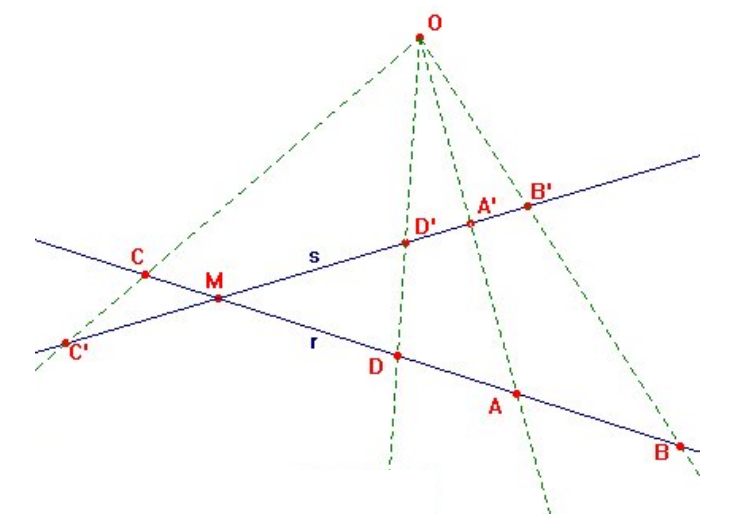
\includegraphics[scale = 0.4]{2.6_1}
\centering
\end{figure}

Esta es la primera de muchas figuras en las que se representarán puntos y rectas como si del plano afín se tratase. Cabe remarcar que se está estudiando geometría proyectiva y no afín; el único propósito de estas figuras es hacerse una idea intuitiva. Todo el asunto de los puntos en el infinito quedará al alcance de la imaginación.

\begin{proposition}
\label{prop2.4.}
    Sean $r,s$ dos rectas de un plano proyectivo.
    \begin{itemize}
        \item[(i)] Toda perspectividad $\pi_O \colon r \to s$ es biyectiva.
        \item[(ii)] La inversa de una perspectividad es otra perspectividad del mismo centro.
        \item[(iii)] Dada una perspectividad, el punto de intersección de $r$ y $s$ es un punto doble, es decir, un punto que se aplica en sí mismo.
        \item[(iv)] Si $r = s$, entonces $\pi_O = id_r$ y cada punto de $r$ es doble.
        \item[(v)] Si $t$ es otra recta del plano proyectivo, entonces
        \[\pi_O(s,t) \circ \pi_O(r,s) = \pi_O(r,t)\]
    \end{itemize}
\end{proposition}

\begin{proof}
    Inmediata.
\end{proof}

\begin{proposition}
\label{prop2.5.}
    Sea $r$ una recta proyectiva sobre el cuerpo $\mathbb{K}$ y sea $\{A,B;C\}$ un sistema de coordenadas homogéneas tal que $A = \ <a>, B = \ <b>, C = \ <a+b>$. Entonces para cada $D \in r$ con $D \neq A$, existe un único $\lambda \in \mathbb{K}$ tal que $D = \ <\lambda a +b>$.
\end{proposition}

\begin{proof}
Supongamos que $D = \ <u>$. Como $\{a,b\}$ es base del espacio vectorial subyacente a la recta proyectiva $r = \overline{AB}$, existen únicos escalares $\alpha, \beta$ tales que $u = \alpha a + \beta b$. Como $D \neq A$, entonces ha de ser $\beta \neq 0$, luego
\[D = \ <u> \ = \ <\alpha a +\beta b> \ = \ <\beta^{-1}(\alpha a + \beta b)> \ = \ <\beta^{-1}\alpha a + b> \ = \ <\lambda a + b> \]
donde $\lambda = \beta^{-1}\alpha$ es el escalar que se buscaba, que además es único por serlo $\beta$ y $\alpha$.
\end{proof}

Nótese que el papel del punto unidad en esta proposición no es más que fijar el sistema de coordenadas homogéneas, pues en la demostración este punto no ha aparecido en escena en ningún momento. Lo que se quiere decir con esto es que lo importante es la elección de los generadores de los puntos base, $a$ y $b$.

\begin{definition}
Del escalar $\lambda$ descrito en la proposición anterior se dirá que es la \ul{abscisa} de $D$ en el sistema en que $A$ está en el infinito, $B$ en el origen y $C$ actúa como punto unidad.
\end{definition}

La interpretación geométrica de todo esto es que la abscisa de $D = (\lambda,1)$ no es más que su coordenada cartesiana en el espacio afín $r \setminus \{A\} \cong \mathbb{K}$ (recuérdese el \hyperref[teo1.1.]{\color{blue}Teorema 1.1}), de ahí que se diga que $A$ es el punto en el infinito (recuérdese la \hyperref[def1.9.]{\color{blue}Definición 1.9}).

\begin{definition}
Sean $A,B,C,D$ cuatro puntos de una recta proyectiva con $A \neq B \neq C \neq A$ y $D \neq A$. Por \ul{razón doble de los cuatro puntos} se entenderá al valor que toma la abscisa $\lambda$ de $D$ en el sistema en que $A$ está en el infinito, $B$ en el origen y $C$ actúa como punto unidad, en cuyo caso se escribirá
\[(ABCD) = \lambda\]
\end{definition}

El hecho de que se verifique $(ABCB) = 0$ y $(ABCC) = 1$ justifica que se diga que el punto $B$ está en el origen y que $C$ actúa como punto unidad.

\begin{theorem}
\label{teo2.2.}
Las perspectividades conservan la razón doble.
\end{theorem}

\begin{proof}
Sea $\pi_O \colon r \to s$ una perspectividad y sean $A,B,C,D \in r$ tales que los tres primeros puntos son distintos entre sí y $D \neq A$. Fíjese el sistema de coordenadas homogéneas $\{A,B;C\}$ y supongamos que 
\[A = \ <a> \qquad B = \ <b> \qquad C = \ <a+b> \qquad O = \ <o> \qquad D = \ <\lambda a +b>\]

Si se denota $A' = \pi_O(A), B' = \pi_O(B), C' = \pi_O(C), D' = \pi_O(D)$, hay que probar que $\{A',B';C'\}$ es un sistema de coordenadas homogéneas adecuado y que $(A'B'C'D') = \lambda$.

\vspace{2mm}
En primer lugar, por ser $\pi_O$ biyectiva, los puntos $A',B',C'$ son distintos entre sí y $D' \neq A'$, lo que significa que $\{A',B';C'\}$ es un sistema de coordenadas homogéneas de $s$ y que tiene sentido considerar la abscisa de $D'$ en dicho sistema.

\vspace{2mm}
Por otro lado, por definición de perspectividad se tiene que $A' \neq O$ y $A' \in \overline{OA} = \ <o,a>$. Razonando como en la demostración de la \hyperref[prop2.5.]{\color{blue}Proposición 2.5}, se tiene que existe un único escalar $\alpha$ con $A' = \ <\alpha o + a>$. Obrando de la misma manera se demuestra la existencia de un único escalar $\beta$ con $B' = \ <\beta o + b>$. Además, $C' \in \overline{A'B'} \cap \overline{OC} = \ <\alpha o + a, \beta o + b> \cap <o,a+b>$, y si escribimos $C' = \ <v>$, entonces existen escalares $x_1,x_2,y_1,y_2$ tales que
\[v = x_1(\alpha o + a) + x_2 (\beta o + b) = y_1 o +y_2(a+b) \implies \begin{cases}
    y_1 = x_1\alpha + x_2\beta \\
    y_2 = x_1 \\
    y_2 = x_2
\end{cases} \implies y_1 = y_2 \alpha + y_2 \beta\]
de donde se deduce que 
\[C' = \ <v> \ = \ < y_2\alpha o + y_2 \beta o + y_2 a + y_2 b > \ = \ <(\alpha + \beta)o + (a+b)> \]

Para terminar, veamos que $D' = (\lambda, 1)$ en el sistema de coordenadas homogéneas $\{A',B';C'\}$. Tenemos que \[D' \in \overline{A'B'} \cap \overline{OD} = \ <\alpha o +a, \beta o +b> \cap <o, \lambda a + b>\] Si se escribe $D' = \ <u>$ y se razona como con $C'$, se concluye que
\[D' = \ <\lambda (\alpha o + a) + (\beta o + b)>\]
luego $D'$ tiene coordenadas homogéneas $(\lambda, 1)$ en el sistema en que $A'$ está en el infinito, $B'$ en el origen y $C'$ actúa como punto unidad. Esto significa que 
\[(\pi_O(A)\pi_O(B)\pi_O(C)\pi_O(D)) = (A'B'C'D') = \lambda\]
como quería demostrarse.
\end{proof}

\begin{theorem}
\label{teo2.3.}
Sea $r$ una recta proyectiva y sea $\mathcal{B} = \{a,b\}$ un sistema de coordenadas homogéneas de $r$. Sean $A = \ <a>, B = \ <b> \ \in r$ y tómense dos puntos $C,D \in r$ tales que $C \notin \{A,B\}, D \neq A$. Si las coordenadas homogéneas de $C$ y $D$ respecto de $\mathcal{B}$ son $(\lambda_0,\lambda_1)$ y $(\mu_0,\mu_1)$, respectivamente, entonces
\[(ABCD) = \frac{\lambda_1 \mu_0}{\lambda_0 \mu_1}\]
\end{theorem}

\begin{proof}
Escríbase $C = \ <c>, D = \ <d>$. Entonces
\[c = \lambda_0 a + \lambda_1 b \qquad d = \mu_0 a + \mu_1 b\]
Para calcular la razón doble $(ABCD)$ hay que considerar $C$ como punto unidad del sistema de coordenadas homogéneas $\{A,B;C\}$, así que conviene escribir $A = \ <\lambda_0 a>$, $B = \ <\lambda_1 b>$. Multiplicando por $\frac{\lambda_1}{\mu_1}$ en la expresión $d = \mu_0 a + \mu_1 b$ se tiene
\[\frac{\lambda_1}{\mu_1} d = \frac{\lambda_1\mu_0}{\mu_1} a + \lambda_1 b\]
y multiplicando y diviendo por $\lambda_0$ el coeficiente de $a$,
\[\frac{\lambda_1}{\mu_1} d = \frac{\lambda_1\mu_0}{\lambda_0 \mu_1} \lambda_0 a + \lambda_1 b\]
de donde se deduce que $\frac{\lambda_1\mu_0}{\lambda_0 \mu_1}$ es la abscisa de $D$, esto es,
\[(ABCD) = \frac{\lambda_1\mu_0}{\lambda_0 \mu_1}\]
Se puede quedar uno tranquilo con el denominador de esta fracción porque $\lambda_0 \mu_1 \neq 0$ al ser $C \neq B$ y $D \neq A$.
\end{proof}

\begin{theorem}
Sea $r$ una recta proyectiva y sea $\mathcal{B} = \{u,v\}$ un sistema de coordenadas homogéneas de $r$. Sean $A,B,C,D \in r$ puntos distintos de los que son conocidas sus abscisas en $\mathcal{B}$, llámense $\alpha, \beta, \gamma, \delta$, respectivamente. Entonces
\[(ABCD) = \frac{(\gamma - \alpha)(\delta - \beta)}{(\delta - \alpha)(\gamma - \beta)}\]
\end{theorem}

\begin{proof}
En primer lugar, se sabe que las coordenadas homogéneas de los puntos en $\mathcal{B}$ son
\[A = (\alpha, 1) \qquad B = (\beta, 1) \qquad C = (\gamma, 1) \qquad D = (\delta, 1)\]
Por tanto, si $A = \ <a>, B = \ <b>, C = \ <c>, D = \ <d>$, se puede escribir
\[a = \alpha u + v \qquad b = \beta u + v \qquad c = \gamma u + v \qquad d = \delta u + v\]
Para calcular la razón doble $(ABCD)$ aplicando el teorema anterior será necesario conocer las coordenadas de $C$ y $D$ en la base integrada por $a$ y $b$, luego es preciso resolver la ecuación vectorial \[c = \lambda_0 a + \lambda_1 b \iff \gamma u + v = \lambda_0 (\alpha u + v) + \lambda_1 (\beta u + v)\]
lo que proporciona el sistema siguiente:
\[\begin{cases}
    \lambda_0 \alpha + \lambda_1 \beta &= \gamma \\
    \lambda_0 \: \: \, + \lambda_1 &= 1
\end{cases}\]
La matriz de coeficientes tiene determinante $\alpha - \beta$, que es no nulo por ser $A \neq B$. Por tanto, resolviendo por la regla de Cramer, se obtiene
\[\lambda_0 = \frac{\gamma - \beta}{\alpha - \beta} \qquad \lambda_1 = \frac{\alpha - \gamma}{\alpha - \beta}\]
Análogamente, si se trata de resolver la ecuación vectorial $d = \mu_0 a + \mu_1 b$, se obtendrá
\[\mu_0 = \frac{\delta - \beta}{\alpha - \beta} \qquad \mu_1 = \frac{\alpha - \delta}{\alpha - \beta}\]
Sustituyendo las ya conocidas coordenadas de $c$ y $d$ en la fórmula proporcionada por el teorema anterior y haciendo cálculos, se llega a la expresión
\[(ABCD) = \frac{(\gamma - \alpha)(\delta - \beta)}{(\delta - \alpha)(\gamma - \beta)}\]
que es lo que se quería probar.
\end{proof}

\begin{theorem}
\label{teo2.5.}
Sea $\sigma \colon r \to s$ una biyección entre rectas proyectivas sobre el mismo cuerpo que preserva razones dobles. Entonces $\sigma$ es una proyectividad.
\end{theorem}

\begin{proof}
Sean $\{A,B;C\}$ y $\{A',B';C'\}$ sistemas de coordenadas homogéneas de $r$ y $s$, respectivamente, y supongamos que las abscisas de $\sigma(A), \sigma(B)$ y $\sigma(C)$ respecto al último de los sistemas existen (el otro caso se estudiará en los ejercicios). Sean $\alpha, \beta$ y $\gamma$ estas abscisas.

\vspace{2mm}
El objetivo es encontrar la ecuación de $\sigma$ y comprobar que se trata de la ecuación de una proyectividad. Primero se hallará esta ecuación en términos de abscisas, y luego de coordenadas homogéneas. 

\vspace{2mm}
Se trata entonces de buscar una relación entre la abscisa $x$ de un punto $X$ y la abscisa $x'$ de su imagen $\sigma(X) = X'$. Supongamos que $X \neq A$. Tiene sentido entonces la abscisa $x = (ABCX)$. Como $\sigma$ preserva razones dobles, se tiene que $x = (ABCX) = (\sigma(A)\sigma(B)\sigma(C)X')$, y por el teorema anterior,
\[x = \frac{(\gamma - \alpha)(x'-\beta)}{(x'-\alpha)(\gamma-\beta)}\]
donde $x' = (A'B'C'X')$. Al multiplicar por $(x'-\alpha)(\gamma-\beta)$ ambos miembros y agrupar adecuadamente los sumandos, se llega a una expresión de la forma
\[(\mu_0 +\mu_1 x)x' = \lambda_0+\lambda_1x\]
para ciertos escalares $\lambda_0,\lambda_1,\mu_0,\mu_1$. Si se pudiera dividir por $\mu_0 +\mu_1x$ se obtendría la ecuación
\[x' = \frac{\lambda_0 + \lambda_1 x}{\mu_0 + \mu_1x}\]
que recibe el nombre de \ul{ecuación explícita} de $\sigma$. Esta ecuación asigna una abscisa a cada punto de $s$, excepto a aquel que sea imagen del punto de $r$ con abscisa $-\frac{\mu_0}{\mu_1}$, llámese $L$. Como el punto que no tiene abscisa es el punto del infinito de $s$ (o sea, $A'$), se concluye que $L$ es aplicado por $\sigma$ en el punto del infinito de $s$.

\vspace{2mm}
Si se tratara de despejar $x$ en la ecuación explícita, un razonamiento análogo permitiría concluir que el punto del infinito de $r$ (o sea, $A$) se transforma en el de $s$ que tiene abscisa $\frac{\lambda_1}{\mu_1}$, al que se llamará $L'$.

\vspace{2mm}
Los puntos $L$ y $L'$ de $r$ y $s$, respectivamente, se denominan \ul{puntos límite}. Finalmente, hay que expresar la ecuación anterior en términos de coordenadas homogéneas. Sea $X = (x_0,x_1)$ un punto de $r$ cuya imagen es $X' = (x_0',x_1')$. Suponiendo que $X$ no es el punto del infinito de $r$ y que $X'$ no es el de $s$, tiene sentido considerar las abscisas de ambos puntos, que serían $x = \frac{x_1}{x_0}$ y $x' = \frac{x_1'}{x_0'}$. Sustituyendo en la ecuación explícita queda
\[\frac{x_0'}{\mu_0x_0+\mu_1x_1} = \frac{x_1'}{\lambda_0x_0+\lambda_1x_1}\]
Sea $\lambda \in \mathbb{K} \setminus \{0\}$ tal que
\[\frac{x_0'}{\mu_0x_0+\mu_1x_1} = \frac{x_1'}{\lambda_0x_0+\lambda_1x_1} = \frac{1}{\lambda}\]
Entonces
\[\begin{cases}
    \displaystyle \frac{1}{\lambda} = \frac{x_0'}{\mu_0x_0+\mu_1x_1} \\
    \\
    \displaystyle\frac{1}{\lambda} = \frac{x_1'}{\lambda_0x_0+\lambda_1x_1}
\end{cases} \iff
\begin{cases}
    \lambda x_0' = \mu_0x_0 + \mu_1x_1 \
    \\
    \lambda x_1' = \lambda_0x_0+\lambda_1x_1
\end{cases} \iff
\lambda \begin{pmatrix*}[r]
    x_0' \\
    x_1'
\end{pmatrix*} = \begin{pmatrix*}[r]
    \mu_0 & \mu_1 \\
    \lambda_0 & \lambda_1
\end{pmatrix*}\begin{pmatrix*}[r]
    x_0 \\
    x_1
\end{pmatrix*}\]

Con el fin de no engorronar la prueba, no se va a calcular el valor de los escalares $\mu_0, \mu_1, \lambda_0, \lambda_1$, pero si se hiciese, se vería que $\mu_0\lambda_1 - \mu_1\lambda_0 \neq 0$, es decir, el determinante de la matriz anterior es no nulo, lo que significa que la ecuación anterior es la ecuación de una proyectividad, como se quería probar.

\vspace{2mm}
Quizá sea inquietante el paradero de los puntos límite en relación a la ecuación anterior, cosa que tampoco se va a investigar, pero si se investigara, se concluiría que la ecuación cuadra perfectamente con sus coordenadas.
\end{proof}

\begin{theorem}
\label{teo2.6.}
Sea $\sigma \colon r \to s$ una proyectividad entre rectas distintas de un mismo plano proyectivo. Entonces $\sigma$ se puede expresar como composición de dos perspectividades.
\end{theorem}

\begin{proof}
Sean $A,B,C \in r$ distintos dos a dos y llámense $A',B',C'$ sus imágenes por $\sigma$. Sean $O$ y $O'$ dos puntos de la recta $\overline{AA'}$ tales que $O \notin r$ y $O' \notin s$. Consideremos los puntos $B'' = \overline{OB} \cap \overline{O'B'}$ y $C'' = \overline{OC} \cap \overline{O'C'}$, la recta $t = \overline{B''C''}$ y el punto $A'' = t \cap \overline{AA'}$. Tómense ahora las perspectividades $\pi_O(r,t)$ y $\pi_{O'}(t,s)$. Entonces
\[(\pi_{O'} \circ \pi_O)(A) = \pi_{O'}(A'') = A'\]
\[(\pi_{O'} \circ \pi_O)(B) = \pi_{O'}(B'') = B'\]
\[(\pi_{O'} \circ \pi_O)(C) = \pi_{O'}(C'') = C'\]
Como consecuencia del teorema anterior, $\pi_{O'} \circ \pi_O$ es una proyectividad, y por el \hyperref[teo2.1.]{\color{blue}Teorema 2.1}, se tiene que $\sigma = \pi_{O'} \circ \pi_O$.
\end{proof}

\begin{figure}[h]
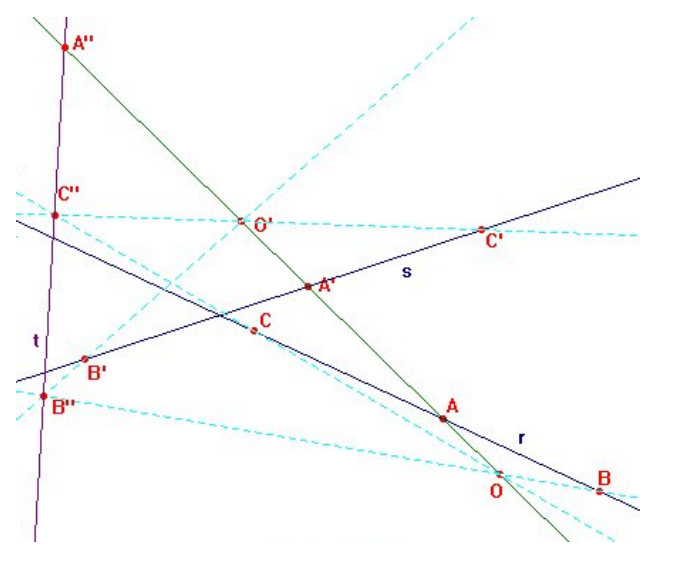
\includegraphics[scale = 0.36]{2.6_2}
\centering
\end{figure}

En la elección de los puntos $O$ y $O'$ de la demostración anterior ha sido fundamental la hipótesis de que las rectas $r$ y $s$ sean distintas. Lo que sucede en el caso $r = s$ lo dirá el siguiente teorema:

\begin{theorem}
\label{teo2.7.}
Sea $\sigma \colon r \to r$ una proyectividad de una recta del plano proyectivo en sí misma. Entonces $\sigma$ se puede expresar como composición de tres perspectividades.
\end{theorem}

\begin{proof}
Sean $A,B,C \in r$ distintos dos a dos. Sea $s$ una recta distinta de $r$ y sea $O$ un punto con $O \notin r$ y $O \notin s$. Considérense la perspectividad $\pi_O(r,s)$, los puntos

\vspace{-4mm}

\setlength{\columnsep}{0cm}
\setlength{\columnseprule}{0pt}

\begin{multicols}{2}

\[A'' = \pi_O(A)\]
\[B'' = \pi_O(B)\]
\[C'' = \pi_O(C)\]

\columnbreak

\[A' = \sigma(A)\]
\[B' = \sigma(B)\]
\[C' = \sigma(C)\]

\end{multicols}
\noindent y la única proyectividad $\tau \colon s \to r$ que envía el símplex $\{A'',B'';C''\}$ en el símplex $\{A',B';C'\}$. Entonces la proyectividad $\tau \circ \pi_O$ manda el símplex $\{A,B;C\}$ en $\{A',B';C'\}$. Por el \hyperref[teo2.1.]{\color{blue}Teorema 2.1}, ha de ser $\tau \circ \pi_O = \sigma$. Por el teorema anterior, se puede descomponer $\tau$ en composición de dos perspectividades $\pi_{O''} \circ \pi_{O'}$, luego $\sigma = \pi_{O''} \circ \pi_{O'} \circ \pi_O$.
\end{proof}

Todos los resultados que han sido probados en esta sección se pueden resumir en el teorema que sigue:

\begin{theorem}
\label{teo2.8.}
Sea $\sigma \colon r \to s$ una biyección entre rectas de un mismo plano proyectivo. Son equivalentes
\begin{itemize}
    \item[(i)] $\sigma$ conserva razones dobles.
    \item[(ii)] $\sigma$ es una proyectividad.
    \item[(iii)] $\sigma$ se descompone en composición de dos perspectividades si las rectas son distintas o de tres perspectividades en caso contrario.
\end{itemize}
\end{theorem}

\begin{proof}
La implicación $(i) \implies (ii)$ se probó en el \hyperref[teo2.5.]{\color{blue}Teorema 2.5}, la implicación $(ii) \implies (iii)$ se probó en el \hyperref[teo2.6.]{\color{blue}Teorema 2.6} y el \hyperref[teo2.7.]{\color{blue}Teorema 2.7} y la implicación $(iii) \implies (i)$ es consecuencia del \hyperref[teo2.2.]{\color{blue}Teorema 2.2}.
\end{proof}

\begin{theorem}
Una proyectividad $\sigma \colon r \to s$ entre rectas del mismo plano proyectivo es una perspectividad si y solo si el punto de intersección de ambas rectas constituye un punto doble.
\end{theorem}

\begin{proof}
Una de las implicaciones se da por probada en la \hyperref[prop2.4.]{\color{blue}Proposición 2.4}. Para el recíproco, supongamos que el punto $A = r \cap s$ es aplicado por $\sigma$ en sí mismo. Tómense $B,C \in r \setminus \{A\}$ puntos distintos y sea $O = \overline{B\sigma(B)} \cap \overline{C\sigma(C)}$. La perspectividad $\pi_O(r,s)$ cumple
\[\pi_O(A) = A = \sigma(A) \qquad \pi_O(B) = \sigma(B) \qquad \pi_O(C) = \sigma(C)\]
y por el \hyperref[teo2.1.]{\color{blue}Teorema 2.1}, tiene que ser $\sigma = \pi_O$.
\end{proof}

\section{Involuciones}

Dada una proyectividad $\sigma \colon r \to s$ entre rectas sobre el mismo cuerpo $\mathbb{K}$ y fijados en ellas dos sistemas de coordenadas, se vio en la demostración del \hyperref[teo2.5.]{\color{blue}Teorema 2.5} que existen $\lambda_0, \lambda_1, \mu_0, \mu_1 \in \mathbb{K}$ con $\lambda_0\mu_1-\lambda_1\mu_0 \neq 0$ y tales que
\[x' = \frac{\lambda_0+\lambda_1x}{\mu_0+\mu_1x}\]
donde $x$ es la abscisa de cualquier punto $X$ distinto del punto límite de $r$, y $x'$ es la abscisa de su imagen, que ha de ser distinta del punto límite de $s$. Haciendo cuentas se obtiene la expresión
\[\lambda xx'+\mu x+\nu x' + \zeta = 0\]
para $\lambda = \mu_1, \mu = -\lambda_1, \nu = \mu_0$ y $\zeta = -\lambda_0$. Se tiene entonces que $\mu v - \lambda \zeta \neq 0$ y que los puntos límite son aquellos con abscisas $x = -\frac{\nu}{\lambda}$ y $x' = -\frac{\mu}{\lambda}$.

\begin{definition}
La expresión anterior se denomina \ul{ecuación general} o \ul{ecuación implícita} de la proyectividad $\sigma$.
\end{definition}

Nótese que la ecuación anterior no es más que un polinomio en $x, x'$, y que el cálculo de los puntos dobles (siempre que tenga sentido, es decir, siempre que $r = s$) se reduce a resolver la ecuación
\[\lambda x^2+(\mu+\nu)x + \zeta = 0\]

\begin{definition}
Si la ecuación anterior tiene dos soluciones, se dirá que la proyectividad $\sigma$ es \ul{hiperbólica}; si solo tuviera una, entonces $\sigma$ será una proyectividad \ul{parabólica}, y en caso de no haberlas, se hablará de proyectividad \ul{elíptica}.
\end{definition}

\begin{definition}
Una proyectividad $\sigma \colon r \to r$ de una recta en sí misma se dirá que es una \ul{involución} cuando $\sigma^2 = id_r$.
\end{definition}

\begin{proposition}
\label{prop2.6.}
Sea $\sigma \colon r \to r$ una proyectividad de una recta en sí misma. Entonces $\sigma$ es una involución distinta de la identidad si y solo si existe $A \in r$ tal que $\sigma(A) \neq A$ y $\sigma^2(A) = A$.
\end{proposition}

\begin{proof}
Una de las implicaciones es trivial, pues si una involución $\sigma$ no fuera la identidad, entonces existiría $A \in r$ tal que $\sigma(A) \neq A$, y por definición de involución sería $\sigma^2(A) = A$.

\vspace{2mm}
Recíprocamente, sea $\sigma$ una proyectividad de una recta en sí misma tal que existe $A \in r$ con $\sigma(A) = B \neq A$ y $\sigma^2(A) = \sigma(B) = A$. Sea $f$ el automorfismo que induce la proyectividad $\sigma$ y escríbase $A = \ <v>$. Como $B = \ <f(v)>$ y $\sigma(B) = A$, entonces existe un escalar no nulo $\lambda$ tal que $f^2(v) = \lambda v$. Consideremos el sistema de coordenadas homogéneas $\{A,B;C\}$, donde $C = \ <v+f(v)>$. Entonces
\begin{itemize}
    \item $\sigma^2(B) = \ <f^2(f(v))> \ = \ <f(f^2(v))> \ = \ <f(\lambda v)> \ = \ <\lambda f(v)> \ = B$
    \item $\sigma^2(C) = \ <f^2(v+f(v))> \ = \ <\lambda v + \lambda f(v)> \ = C$
\end{itemize}
luego $\sigma^2$ deja invariante al símplex $\{A,B;C\}$. Por el \hyperref[teo2.1.]{\color{blue}Teorema 2.1}, ha de ser $\sigma^2 = id_r$, así que $\sigma$ es una involución distinta de la identidad.
\end{proof}

\begin{proposition}
Una proyectividad $\sigma \colon r \to r$ distinta de la identidad es una involución si y solo si su ecuación general es de la forma
\[\lambda x x' + \mu(x+x')+\zeta = 0\]
\end{proposition}

\begin{proof}
Sea $\sigma \colon r \to r$ una involución distinta de la identidad y considérese su ecuación general:
\[\lambda x x'+\mu x + \nu x' + \zeta = 0\]
Si $x$ es la abscisa de un punto de $r$ y $x'$ la de su imagen, por ser $\sigma$ una involución se tiene que el punto de abscisa $x'$ es enviado en el punto de abscisa $x$, así que se satisface la ecuación
\[\lambda x' x+\mu x' + \nu x + \zeta = 0\]
Restando estas dos últimas ecuaciones se obtiene $(\mu - \nu)(x' - x) = 0$. Como $\sigma$ no es la identidad, tomando cualquier punto con abscisa $x$ que no sea doble ($x' \neq x$) se obtiene $\nu = \mu$.

\vspace{2mm}
Recíprocamente, supóngase que una proyectividad $\sigma \colon r \to r$ distinta de la identidad tiene como ecuación
\[\lambda x x' + \mu(x+x')+\zeta = 0\]
Sea $\beta$ la abscisa de un punto $B$ de $r$ y $\beta'$ la de su imagen, $B' = \sigma(B)$. Se puede suponer $B \neq B'$ por no ser $\sigma$ la identidad. Entonces
\[\lambda \beta \beta' + \mu(\beta+\beta')+\zeta = 0 \iff \lambda \beta' \beta + \mu(\beta' + \beta) + \zeta = 0\]
y esto implica que $\sigma(B') = B$, es decir, $\sigma^2(B) = B$. La proposición anterior termina la prueba.
\end{proof}

\section{Segundo teorema de Desargues}

\begin{definition}
Por \ul{cuadrivértice} se entiende a un símplex de un plano proyectivo, es decir, un conjunto de puntos $\{A,B,C,D\}$ llamados \ul{vértices} tales que no hay tres de ellos alineados.
\end{definition}

\begin{definition}
Sea $\{A,B,C,D\}$ un cuadrivértice de un plano proyectivo y considérense las seis rectas que determinan estos puntos. Sean $\overline{AB}, \overline{AC}, \overline{AD}, \overline{BC}, \overline{BD}, \overline{CD}$ estas seis rectas, las cuales se intersecan en los cuatro vértices de partida y en los puntos
\[E = \overline{AB} \cap \overline{CD}  \qquad F = \overline{AC} \cap \overline{BD} \qquad G = \overline{AD} \cap \overline{BC} \]
A estos tres puntos se les llama \ul{puntos diagonales}.
\end{definition}

\begin{definition}
Por \ul{cuadrilátero} se entenderá al concepto dual de cuadrivértice, es decir, a un conjunto de rectas $\{a,b,c,d\}$ de un plano proyectivo tales que no haya tres de ellas concurrentes. A tales rectas se les conocerá como \ul{lados} del cuadrilátero.
\end{definition}

\begin{definition}
Sea $\{a,b,c,d\}$ un cuadrilátero de un plano proyectivo y considérense los siete puntos en los que se intersecan los cuadro lados, que determinan un total de siete rectas. A las rectas
\[e = \overline{(a \cap b) (c \cap d)} \qquad f = \overline{(a \cap c) (b \cap d)} \qquad g = \overline{(a \cap d) (b \cap c)}\]
se les denomina \ul{rectas diagonales}.
\end{definition}

\begin{figure}[h]
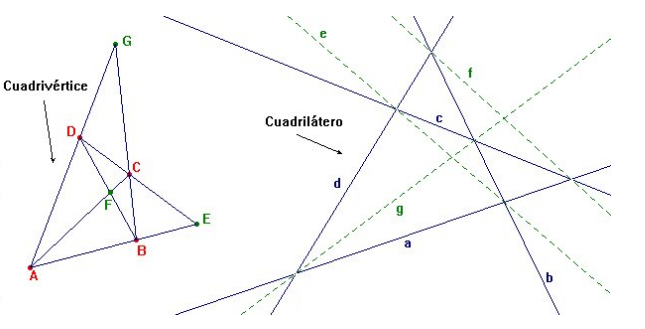
\includegraphics[scale = 0.7]{2.8_1}
\centering
\end{figure}

\begin{theorem}[Segundo teorema de Desargues]
Sea $\{A,B,C,D\}$ un cuadrivértice de un plano proyectivo y sea $r$ una recta de dicho plano que no contiene a ninguno de los vértices. Si consideramos los puntos
\[P = r \cap \overline{BC} \quad P' = r \cap \overline{AD} \quad Q = r \cap \overline{AB} \quad Q' = r \cap \overline{CD} \quad R = r \cap \overline{BD} \quad R' = r \cap \overline{AC}\]
entonces la única proyectividad $\sigma \colon r \to r$ que aplica $P$ en $P'$, $Q$ en $Q'$ y $R$ en $R'$ es una involución.
\end{theorem}


\begin{figure}[h]
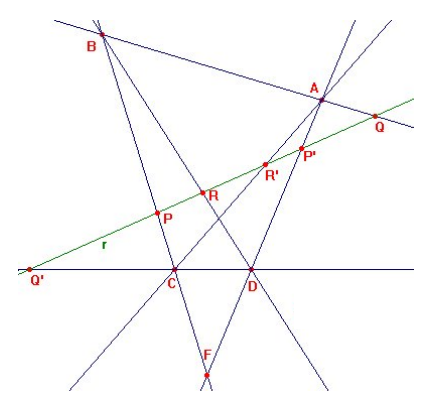
\includegraphics[scale = 0.6]{2.8_2}
\centering
\end{figure}

\begin{proof}
Supóngase que uno de los puntos no se transforma en sí mismo, por ejemplo $P \neq P' = \sigma(P)$. La perspectividad $\pi_B(r,\overline{AD})$ verifica

\setlength{\columnsep}{0cm}
\setlength{\columnseprule}{0pt}

\begin{multicols}{2}

\begin{itemize}
    \item $\pi_B(Q) = \overline{BQ} \cap \overline{AD} = A$
    \item $\pi_B(R) = \overline{BR} \cap \overline{AD} = D$
\end{itemize}

\columnbreak

\begin{itemize}
    \item $\pi_B(P) = \overline{BC} \cap \overline{AD}$
    \item $\pi_B(P') = \overline{BP'} \cap \overline{AD} = P'$
\end{itemize}

\end{multicols}
Se llamará $F$ al punto $\overline{BC} \cap \overline{AD}$. Por el \hyperref[teo2.8.]{\color{blue}Teorema 2.8}, se tiene que $(QRPP') = (ADFP')$. Razonando de la misma forma con la perspectividad $\pi_C(r,\overline{AD})$ se obtiene la igualdad $(R'Q'PP') = (ADFP')$. Un cálculo sencillo usando las fórmulas vistas para las abscisas prueba que para puntos $A,B,C,D$ cualesquiera distintos dos a dos se cumple que
\[(ABCD) = (BADC)\]
En particular, $(R'Q'PP') = (Q'R'P'P)$. Como $\sigma$ preserva razones dobles, entonces también se tiene $(QRPP') = (Q'R'P'\sigma(P'))$. Esto significa que $\sigma(P')$ tiene la misma abscisa que $P$ en el sistema de coordenadas homogéneas $\{Q',R';P'\}$. Por la unicidad de la abscisa, se tiene $\sigma(P') = P$, es decir, $\sigma^2(P) = P$, y la \hyperref[prop2.6.]{\color{blue}Proposición 2.6} hace de $\sigma$ una involución.

\vspace{2mm}
Falta razonar el caso en que $P = P', R = R'$ y $Q = Q'$. En tal situación, el \hyperref[teo2.1.]{\color{blue}Teorema 2.1} obliga a que sea $\sigma = id_r$, que es una involución.
\end{proof}

\section{Teorema de Fano}

Se recuerda que la \ul{característica} de un anillo $R$ es el menor $n \in \N$ para el que se tiene $na=0 \ \, \forall \ a \in R$. En caso de no existir un tal natural, se dice que la característica de $R$ es cero.

\begin{theorem}[Teorema de Fano]
Los tres puntos diagonales de un cuadrivértice sobre un plano proyectivo están alineados si y solo si la característica del cuerpo base es $2$.
\end{theorem}

\begin{proof}
\hfill
\begin{itemize}
    \item[{\fbox[rb]{$\Rightarrow$}}] Sean $A = \ <a>, B = \ <b>, C = \ <c>, D = \ <d>$ puntos de un cuadrivértice en un plano proyectivo sobre el cuerpo $\mathbb{K}$ tales que los puntos diagonales están alineados. Se puede escribir $D = \ <a+b+c>$, y por tanto se tiene que \[< a+b> \ = \ <(a+b+c)-c> \ \in \overline{AB} \cap \overline{CD}\] Como $E = \overline{AB} \cap \overline{CD}$, entonces debe ser $E = \ <a+b>$. Razonando de la misma forma se obtiene
    \[G = \ <a+c> \ = \ <(a+b+c)-b> \ = \overline{AC} \cap \overline{BD} \]
    \[F = \ <b+c> \ = \ <(a+b+c)-a> \ = \overline{BC} \cap \overline{AD} \]
    Los tres puntos están alineados, así que $F \in \overline{EG}$, y por tanto $b+c$ se puede expresar como combinación lineal de $a+b$ y $a+c$:
    \[b+c = \lambda(a+b)+\mu(a+c) = (\lambda+\mu)a+\lambda b + \mu c\]
    Se concluye que $\lambda = \mu = 1$ y también $\lambda + \mu = 0$, es decir $1+1 = 2 = 0$, por lo que $\mathbb{K}$ tiene característica $2$.
    \item[{\fbox[rb]{$\Leftarrow$}}] Sean $A = \ <a>, B = \ <b>, C = \ <c>, D = \ <d>$ puntos de un cuadrivértice en un plano proyectivo sobre un cuerpo $\mathbb{K}$ de característica $2$. Por la implicación anterior se sabe que los puntos diagonales son $E = \ <a+b>, \, F = \ <b+c>, \, G = <a+c>$. Además,
    \[<b+c> \ = \ <(a+b)+(a+c)> \]
    luego $F \in \overline{EG}$, así que los puntos diagonales están alineados.
\end{itemize}
\end{proof}

Aprovechando todo esto de los cuadrivértices y los puntos diagonales, se darán un par de definiciones sobre las que se trabajará en alguno de los ejercicios:

\begin{definition}
En un plano afín, un \ul{trapecio} se define como un cuadrivértice con un punto diagonal en el infinito, y un \ul{palalelogramo} se define como un cuadrilátero con dos de sus puntos diagonales en el infinito.
\end{definition}

\section{Cuaterna armónica}

\begin{proposition}
Sea $\{A,B,F,E\}$ un cuadrivértice de un plano proyectivo $\mathcal{P}$ de puntos diagonales $C = \overline{AB} \cap \overline{EF}$, $G = \overline{AE} \cap \overline{BF}$ y $L = \overline{AF} \cap \overline{BE}$. Sea $D = \overline{GL} \cap \overline{AB}$. Entonces $(ABCD) = -1$.
\end{proposition}

\begin{proof}
En primer lugar, los puntos $A,B,C,D$ están alineados y son distintos, y por tanto tiene sentido considerar su razón doble. Por la perspectividad $\pi_G(\overline{AB}, \overline{EF})$ se tiene que $(ABCD)=(EFCH)$, donde $H = \overline{EC} \cap \overline{GD}$, y por la perspectividad $\pi_L(\overline{EF}, \overline{AB})$ se tiene que $(EFCH)=(BACD)$, luego $(ABCD) = (BACD)$. Haciendo cálculos con las fórmulas de las abscisas se concluiría que o bien $(ABCD) = 1$ o bien $(ABCD) = -1$. En el primer caso se tendría que $D = C$ y el teorema de Fano diría que el cuerpo base tiene característica 2, luego 1 = -1. En el segundo caso no queda nada que probar.
\end{proof}

\begin{figure}[h]
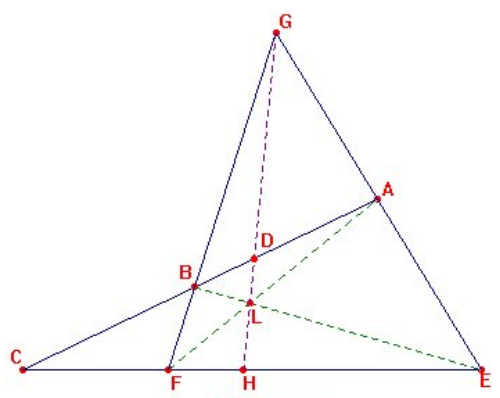
\includegraphics[scale = 0.5]{2.9_1}
\centering
\end{figure}

\begin{definition}
Los elementos de una cuaterna $(A, B, C, D)$ de puntos de una recta proyectiva se dirá que están en \ul{cuaterna armónica} si $(ABCD) = -1$. En tal situación, a $D$ se le llamará \ul{cuarto armónico} de la terna $(A,B,C)$, y a $C$ y $D$ se les denominará \ul{conjugados armónicos} de $A$ y $B$.
\end{definition}

Una extensa retahíla de cálculos usando las fórmulas vistas para las abscisas demostraría que la definición es buena, en el sentido de que da igual el orden en que se den los puntos.

\begin{definition}
Si $P,Q$ son puntos de un espacio afín $\mathcal{A}(V,H)$, se define su \ul{punto medio} como
\[\lambda(R) = \frac{\lambda(P)+\lambda(Q)}{2}\]
donde $\displaystyle \lambda \colon \mathcal{A}(V,H) \to \mathbb{K}^n$ es la aplicación definida en el \hyperref[teo1.1.]{\color{blue}Teorema 1.1}, es decir, $\lambda(A)$ son las coordenadas cartesianas de $A$ para todo $A \in \mathcal{A}(V,H)$.
\end{definition}

El $2$ en el denominador parece inofensivo pero podría ocurrir que el cuerpo base tuviera característica $2$. Es por ello que de aquí en adelante no se trabajará con estos cuerpos.

\vspace{2mm}
Recuérdese además que en el caso de rectas proyectivas, la coordenada cartesiana de cualquier punto $D$ perteneciente a un afín $r \setminus \{A\}$ es precisamente su abscisa. En este caso, todo esto de los puntos medios depende del punto $A$ que esté en el infinito.

\begin{proposition}
Cuatro puntos $(A, B, C, D)$ distintos de una recta proyectiva $r$ están en cuaterna armónica si y solo si $B$ se encuentra en el punto medio de $C$ y $D$ en el espacio afín $r \setminus \{A\}$.
\end{proposition}

\begin{proof}
 \hfill
\begin{itemize}
    \item[{\fbox[rb]{$\Rightarrow$}}] En el sistema en que $A$ está en el infinito, $B$ en el origen y $C$ actúa como punto unidad, se tiene que
    \[(ABCB) = 0 \qquad (ABCC) = 1\]
    Como por hipótesis es $(ABCD) = -1$, entonces
    \[0 = \lambda (B) = \frac{\lambda(C)+\lambda(D)}{2} = \frac{1 -1}{2}\]
    \item[{\fbox[rb]{$\Leftarrow$}}] Escribimos $A = \ <a>, B = \ <b>, C = \ <a+b>, D = \ < \mu a +b>$, donde $\mu$ es la abscisa de $D$, y suponemos que $B$ es el punto medio de $C$ y $D$ en el afín $r \setminus \{A\}$. Respecto al sistema de coordenadas $\{A,B;C\}$, los cuatro puntos tienen coordenadas homogéneas
    \[A = (1,0) \qquad B = (0,1) \qquad C = (1,1) \qquad D = (\mu,1)\]
    Ahora bien, por hipótesis se tiene que $0 = 2 \cdot 0 = 2 \cdot \lambda(B) = \lambda(C) + \lambda(D) = 1+\mu$, luego tiene que ser $\mu = -1$.
\end{itemize}
\end{proof}


\section{Transformaciones entre haces de rectas}

En esta sección se tratará de dualizar una parte de todo lo visto en las secciones anteriores. Los espacios proyectivos considerados serán planos proyectivos.

\vspace{2mm}
Lo primero que se dualizará es aquella configuración de cuatro puntos alineados $A,B,C,D$ de forma que los tres primeros sean distintos entre sí y que $D \neq A$:

\begin{definition}
Se entiende por \ul{lápiz} a cuatro rectas $\{a,b,c,d\}$ concurrentes de un plano proyectivo con $a \neq b \neq c \neq a \neq d$.
\end{definition}

\begin{definition}
Un lápiz $\{a,b,c,d\}$ se dirá que es \ul{armónico} si existe un cuadrilátero que tenga a $a$ y $b$ como dos de sus lados, a $c$ como una de sus diagonales y a $d$ de forma que pase por el punto de corte de las otras dos diagonales.
\end{definition}

Los conceptos duales de aplicaciones entre rectas (un conjunto de puntos alineados) serán aplicaciones entre haces de rectas concurrentes (un conjunto de rectas que pasan por un punto dado). Si $A$ es un punto de un plano proyectivo $\mathcal{P}$, se denotará por $A^*$ al haz de rectas de $\mathcal{P^*}$ que pasan por $A$.

\begin{definition}
Si $A^*$ y $B^*$ son haces de rectas de un mismo plano y $r$ es una recta de dicho plano con $A \notin r$ y $B \notin$ r, se define la \ul{perspectividad de eje $r$} como la aplicación
\[
\begin{aligned}[t]
\pi_r \colon A^* &\longrightarrow B^* \\
a &\longmapsto \pi_r(a) = \overline{(a \cap r)B}
\end{aligned}
\]
\end{definition}

\begin{definition}
Una aplicación entre haces de rectas del mismo plano es una \ul{proyectividad} si es composición de un número finito de perspectividades.
\end{definition}

\begin{definition}
Se define la \ul{razón doble} de un lápiz $\{a,b,c,d\}$ como
\[(abcd) = (a^* b^* c^* d^*)\]
donde $a^*, b^*, c^*, d^*$ son las imágenes de $a, b, c, d$ por la correlación estándar.
\end{definition}

\begin{example}
En el plano proyectivo sobre $\R$, se consideran el punto $P = \ <(1,0,1)>$ y las rectas
\[
\begin{aligned}
a &\equiv x_0-2x_1-x_2=0\\
b &\equiv 2x_0-2x_2=0\\
c &\equiv x_0+x_1-x_2=0\\
d &\equiv 5x_0-3x_1-5x_2=0\\
\end{aligned}
\]
Se comprueba fácilmente que $\{a,b,c,d\}$ es un lápiz concurrente en $P$. Se trata de calcular $(abcd)$. Si se recuerda el \hyperref[teo0.4.]{\color{blue}Teorema 0.4}, se tiene que
\[
\begin{aligned}
a^\circ &= \ <(1,-2,-1)>\\
b^\circ &= \ <(2,0,-2)>\\
c^\circ &= \ <(1,1,-1)>\\
d^\circ &= \ <(5,-3,-5)>\\
\end{aligned}
\]
Por comodidad, se llamará $A, B, C $ y $D$ los cuatro puntos anteriores. Habrá que expresar ahora el vector $(1,1,-1)$ como combinación lineal de $(1,-2,-1)$ y $(2,0,-2)$. La ecuación vectorial
\[(1,1,-1) = \lambda_0(1,-2,-1)+\lambda_1(2,0,-1) \]
tiene como solución $\lambda_0 = -1/2, \lambda_1 = 3/4$. Por tanto, respecto al sistema de coordenadas homogéneas $\{(-1/2,1,1/2), (3/2,0,-3/2)\}$, el punto $c^\circ$ tiene coordenadas $(1,1,1)$. Queda expresar el generador de $D$ como combinación lineal de los dos vectores del sistema de coordenadas homogéneas. La ecuación vectorial
\[(5,-3,-5) = \alpha (-1/2,1,1/2)+\beta(3/2,0,-3/2)\]
proporciona los coeficientes $\alpha = -3, \beta = 7/3$. En coordenadas homogéneas se tiene que $D = (-3,7/3) = (-9/7,1)$, luego
\[-\frac{9}{7} = (ABCD) = (abcd)\]
\end{example}

Como alternativa a realizar estos cálculos, quizá sea más fácil aplicar directamente el siguiente teorema:

\begin{theorem}
Sea $\{a,b,c,d\}$ un lápiz de un plano proyectivo y $r$ una recta que no pase por $a \cap b$. Entonces $(abcd) = (ABCD)$, donde $A = a \cap r, B = b \cap r, C = c \cap r, D = d \cap r$.
\end{theorem}

\begin{proof}
Ejercicio.
\end{proof}

\begin{example}
Volviendo al ejemplo anterior y tomando $r \equiv x_0 = 0$, se tiene que
\[
\begin{aligned}
P &= a \cap r = \ <(0,1,-2)>\\
Q &= b \cap r = \ <(0,1,0)>\\
R &= c \cap r = \ <(0,1,1)>\\
S &= d \cap r = \ <(0,5,-3)>\\
\end{aligned}
\]
Consideremos el sistema de coordenadas homogéneas $\{(0,1,-2),(0,1,0)\}$. Si se trata de expresar el generador del punto $R$ como combinación lineal de los de $P$ y $Q$, se obtiene la ecuación vectorial
\[(0,1,1) = \lambda_0(0,1,-2)+\lambda_1(0,1,0)\]
Esto implica $\lambda_0 = -1/2$, $\lambda_1 = 3/2$. Por otro lado, escribiendo
\[(0,5,-3) = \mu_0(0,1,-2)+\mu_1(0,1,0)\]
se obtiene $\mu_0 = 3/2, \mu_1 = 7/2$. Por el \hyperref[teo2.3.]{\color{blue}Teorema 2.3} y el teorema anterior,
\[(PQRS) = (abcd) = \frac{\frac{3}{2}\frac{3}{2}}{-\frac{1}{2}\frac{7}{2}} = -\frac{9}{7}\]
\end{example}

El siguiente teorema reúne todos los resultados correspondientes a la dualización de los que ya se conocen:

\pagebreak

\begin{theorem}
\hfill
\begin{itemize}
    \item[(i)] Toda proyectividad entre haces de un mismo plano se expresa como composición de a lo sumo tres perspectividades.
    \item[(ii)] Las proyectividades entre haces de rectas de un mismo plano conservan razones dobles de lápices.
    \item[(iii)] Toda biyección entre haces de rectas de un mismo plano que conserve razones dobles de lápices es una perspectividad.
    \item[(iv)] Una proyectividad $\sigma$ entre haces de rectas $A^*$ y $B^*$ de un plano es una perspectividad si y solo $\sigma(\overline{AB}) = \overline{AB}$, es decir, si y solo si la recta $\overline{AB}$ es doble.
    \item[(v)] Una proyectividad $\sigma$ de un haz de rectas en sí mismo es una involución distinta de la identidad si y solo si existe una recta $a$ del haz tal que $\sigma(a) \neq a$ y $\sigma(a)^2 = a$.
    \item[(vi)] Una involución en un haz distinta de la identidad tiene, a lo sumo, dos rectas dobles.
\end{itemize}
\end{theorem}

\chapter{Teoremas de configuración}

\section{Homologías, homotecias y traslaciones}

En esta sección se estudiarán las proyectividades de un plano proyectivo en sí mismo. Todo espacio proyectivo que aparezca en esta sección será bidimensional.

\begin{definition}
A las rectas invariantes por proyectividades se les llamará \ul{rectas dobles}. En general, los subespacios invariantes por proyectividades se dirán \ul{subespacios dobles}.
\end{definition}

Se advierte que el hecho de que una recta sea doble no significa que todos los puntos de la misma sean puntos dobles. Ahora bien...

\begin{proposition}
\label{prop3.1.}
Sea $\sigma \colon \mathcal{P} \to \mathcal{P}$ una proyectividad.
\begin{itemize}
    \item[(i)] Si $r$ y $s$ son rectas dobles distintas, entonces $r \cap s$ es punto doble.
    \item[(ii)] Si $A$ y $B$ son puntos dobles distintos, entonces $\overline{AB}$ es recta doble.
\end{itemize}
\end{proposition}

\begin{proof}
\hfill
\begin{itemize}
    \item[(i)] Si $r$ y $s$ son dobles por $\sigma$, entonces $\sigma(r \cap s) = \sigma(r) \cap \sigma(s) = r \cap s$.
    \item[(ii)] Si $A$  y $B$ son dobles por $\sigma$ y $X \in \overline{AB}$, entonces $\sigma(X) \in \overline{\sigma(A)\sigma(B)} = \overline{AB}$.
\end{itemize}
Nótese que el segundo apartado es la situación dual del primero.
\end{proof}

\begin{definition}
Una proyectividad $\sigma \colon \mathcal{P} \to \mathcal{P}$ es \ul{central} si existe un punto $C$ tal que $\sigma(\overline{CX}) = \overline{CX}$ para todo $X \neq C$, es decir, tal que toda recta por $C$ es doble. De $C$ se dirá que es el \ul{centro} de la proyectividad.
\end{definition}


\begin{proposition}
\label{prop3.2.}
Sea $\sigma \colon \mathcal{P} \to \mathcal{P}$ una proyectividad.
\begin{itemize}
    \item[(i)] Si hay en $\mathcal{P}$ dos rectas distintas llenas de puntos dobles, entonces $\sigma$ es la identidad.
    \item[(ii)] Si $C$ es un centro de $\sigma$, entonces $C$ es doble.
    \item[(iii)] Si $\sigma$ tiene dos centros distintos, entonces es la identidad.
    \item[(iv)] Si $C$ es un centro de $\sigma$ y $r$ es una recta doble que no pasa por $C$, entonces todo punto de $r$ es doble.
\end{itemize}
\end{proposition}

\begin{proof}
\hfill
\begin{itemize}
    \item[(i)] Sean $r$ y $s$ rectas distintas con todos sus puntos dobles y sean $A,B \in r \setminus s$, $C,D \in s \setminus r$. Entonces no hay tres de estos cuatro puntos alineados, luego $\{A,B,C,D\}$ es un símplex del plano que queda invariante por $\sigma$. El \hyperref[teo2.1.]{\color{blue}Teorema 2.1} dice que $\sigma$ es la identidad.

    \vspace{2mm}
    En este argumento supondría un problema que las rectas solo tuviesen dos puntos. Si se echa un vistazo al Ejercicio 10 del tema anterior se puede concluir que si $\mathbb{K}$ tuviera al menos dos elementos ($q \geq 2$) entonces las rectas tendrían al menos dos puntos. Ahora bien, esto siempre es cierto, pues $0, 1 \in \mathbb{K}$, lo que valida el argumento anterior.
    
    \item[(ii)] Basta tomar dos rectas diferentes por $C$ y usar la \hyperref[prop3.1.]{\color{blue}Proposición 3.1} para concluir que el centro es un punto doble.
\end{itemize}
El resto de la prueba se hará en los ejercicios.
\end{proof}

\begin{definition}
Una \ul{homología} es una proyectividad central de un plano en sí mismo distinta de la identidad.
\end{definition}

De (iii) de la proposición precedente se deduce que para toda homología existe un único punto tal que toda recta por él es doble. La situación dual se recoge en el siguiente teorema:

\begin{theorem}
Toda homología posee una única recta llena de puntos dobles.
\end{theorem}

\begin{proof}
Sea $\sigma$ una homología del plano $\mathcal{P}$ con centro $C$. El apartado (i) de la proposición anterior hace que solo sea necesario probar la existencia. 

\vspace{2mm}
Como $\sigma$ no es la identidad, se puede tomar un punto $P$ con $\sigma(P) \neq P$. Como $C$ es doble, se tiene que $P \neq C$, lo que permite considerar la recta doble $\overline{PC}$. Sea $r$ otra recta que pase por $P$ y distinta de $\overline{PC}$. No puede ser $\sigma(r) = r$ porque entonces se tendría $\sigma(P) = P$, ya que la intersección de rectas dobles es un punto doble. Considérese el punto $A = r \cap \sigma(r)$. Entonces $A \neq C$ (pues $C \notin r$), así que puede escribirse $A = r \cap \overline{AC}$, con $\overline{AC}$ recta doble. Se tiene que $\sigma(A) \in \sigma(r)$ y $\sigma(A) \in \sigma(\overline{AC}) = \overline{AC}$, de donde se concluye que $A = \sigma(r) \cap \overline{AC} = \sigma(A)$.

\vspace{2mm}
Tómese ahora otra recta $s$ que pase por $P$ distinta de $\overline{PC}$ y de $r$. Repitiendo la argumentación del párrafo anterior se encuentra el punto doble $B = s \cap \sigma(s)$, que es distinto de $A$ por ser $r \neq s$. El apartado (ii) de la la \hyperref[prop3.1.]{\color{blue}Proposición 3.1} obliga a que la recta $\overline{AB}$ sea doble. Ahora se presenta la siguiente disyuntiva:
\begin{itemize}
    \item[(i)] Si $C \notin \overline{AB}$, el cuarto apartado de la proposición anterior dice que todo punto de $\overline{AB}$ es doble.
    \item[(ii)] Si $C \in \overline{AB}$, entonces $\bigl.\sigma\bigr|_{\overline{AB}}$ deja invariante al símplex $\{A, B, C\}$ de la recta $\overline{AB}$. Por el \hyperref[teo2.1.]{\color{blue}Teorema 2.1}, se tiene que $\bigl.\sigma\bigr|_{\overline{AB}}$ es la identidad, luego todo punto de $\overline{AB}$ es doble.
\end{itemize}
En cualquiera de los casos, la demostración está terminada.
\end{proof}

\begin{definition}
Dada una homología, la recta constituida por puntos dobles cuya existencia y unicidad asegura el teorema anterior es denominada \ul{eje de la homología}.
\end{definition}

\begin{proposition}
\label{prop3.3.}
Una homología $\sigma$ queda determinada por completo al dar su centro $C$, su eje $r$, un punto $A$ con $A \neq C$ y $A \notin r$, y su imagen $A' = \sigma(A)$.
\end{proposition}

\begin{proof}
En tales circunstancias, si se quiere hallar la imagen de cualquier otro punto $B \neq C$ con $B \notin r \cup \overline{CA}$, se considera el punto $P = r \cap \overline{AB}$. Entonces $B' = \sigma(B) \in \overline{CB}$ por ser esta recta doble, y también $\sigma(B) \in \sigma(\overline{AP}) = \overline{A'P}$. Por tanto, $B' = \overline{CB} \cap \overline{A'P}$ (si fuese $B \in \overline{CA}$ esta intersección no sirve). Con esto queda determinada la imagen de $B$.

\vspace{2mm}
Supóngase ahora que $D \in \overline{CA}$. En este caso se toma cualquier punto $B \notin r \cup \overline{CA}$ y se construye su imagen como antes. Sea $Q = \overline{BD} \cap r$. Entonces $\sigma(D) = D' = \overline{CD} \cap \overline{B'Q}$, lo que determina la imagen de $D$.
\end{proof}

A continuación, se estudiará en qué situaciones las homologías pueden ser restringidas al espacio afín.

\begin{proposition}
\label{prop3.4.}
Sean $\mathcal{P}$ un plano proyectivo, $\sigma$ una homología de centro $C$ y eje $r$ y $s$ la recta del infinito del afín $\mathcal{A} = \mathcal{P} \setminus s$. Si $\sigma$ se restringe al espacio afín $\mathcal{A}$, entonces $\sigma(s) = s$ y además se da una de las siguientes posibilidades:
\begin{itemize}
    \item[(i)] $C \in \mathcal{A}$ y $r = s$.
    \item[(ii)] $C \in r$ y $r = s$.
    \item[(iii)] $C \in s$ y $C \notin r$.
    \item[(iv)] $r \neq s$ y $C = r \cap s$.
\end{itemize}
\end{proposition}
\begin{proof}
Veamos primero que $\sigma(s) = s$. Que $\sigma$ se restrinja al afín significa que
\[
\begin{aligned}[t]
\biggl[ P \in \mathcal{A} \implies \sigma(P) \in \mathcal{A} \ \forall \ P \in \mathcal{P}\biggr] &\iff \biggl[ P \notin s \implies \sigma(P) \notin s \ \forall \ P \in \mathcal{P}\biggr] \\
&\iff \biggl[ \sigma(P) \in s \implies P \in s \ \forall \ P \in \mathcal{P}\biggr] \\
&\iff \sigma(s) = s
\end{aligned}
\]
luego la recta del infinito es doble. Ahora se distinguen dos situaciones:
\begin{itemize}
    \item[I.] Si $C \in \mathcal{A}$, veamos que debe ser $r = s$. Si se diese lo contrario, se tendría que $s$ es recta doble y $C \notin s$ por estar en el afín. Por el apartado cuarto de la \hyperref[prop3.2.]{\color{blue}Proposición 3.2}, todo punto de $s$ es doble. Se tendrían pues dos rectas distintas llenas de puntos dobles ($r$ y $s$), luego $\sigma = id$, que es imposible. La conclusión es que en este caso se cumple (i).
    \item[II.] Si $C \notin \mathcal{A}$, entonces $C \in s$. De nuevo, se presentan dos casos:
    \begin{itemize}
        \item[II.1.] Si $r = s$, entonces $C \in r$, luego se da (ii).
        \item[II.2.] Si $r \neq s$, entonces o bien $C \in r$, en cuyo caso se cumple $C \in r \cap s$ y por tanto sería cierto (iv), o bien $C \notin r$, lo que supondría (iii).
    \end{itemize}
\end{itemize}
Esto agota todos los casos y la demostración está terminada.
\end{proof}

De entre los cuatro panoramas descritos en la proposición anterior, aquí serán estudiados los dos primeros, dejando el resto para los ejercicios. En cuanto a (i)...

\begin{definition}
Si $C$ es un punto de un plano afín, por \ul{homotecia de centro $C$} se entiende a una afinidad que, o bien es la identidad, o bien es la restricción de una homología $\sigma \colon \mathcal{P} \to \mathcal{P}$ de centro $C \in \mathcal{A}$ y eje la recta del infinito.
\end{definition}

\begin{theorem}[Teorema de Tales]
Para cada homotecia $\sigma$ de centro $C$, existe un escalar $\lambda$ tal que para todo punto $X$ del afín se tiene
\[\sigma(X) - C = \lambda(X - C)\]
Además, para cada par de puntos $X,Y$ del afín,
\[\sigma(X)-\sigma(Y)=\lambda(X-Y)\]
\end{theorem}

\begin{proof}
Si la homotecia es la identidad, no hay más que poner $\lambda = 1$. En otro caso, se toma un punto $A$ del afín con $A \neq \sigma(A) =A' \in \overline{CA}$ (nótese que $\overline{CA}$ es una recta porque $C$ es doble y $A$ no, luego $A \neq C$). Sea $B \notin \overline{CA}$ y sea $B' = \sigma(B)$. Como $A' \in \overline{AC}$, se puede escribir $A' - C= \lambda(A-C)$ para algún escalar $\lambda$. Por la misma razón, existe algún escalar $\mu$ con $B'-C=\mu(B-C)$. El decimonoveno ejercicio del tema anterior permite escribir $\lambda = (QCAA')$ y $\mu = (RCBB')$ donde $Q$ es el punto del infinito de $\overline{CA}$ y $R$ el de $\overline{CB}$. Considerando la perspectividad $\pi_P(\overline{AC}, \overline{AB})$ con $P = \overline{AB} \cap \overline{A'B'}$, se tiene que $\lambda = \mu$ por conservar las perspectividades las razones dobles. 

\vspace{2mm}
El caso $X \in \overline{CA}$ se deja como ejercicio. Por último, si $X,Y$ son puntos del espacio afín, entonces
\[\sigma(X)-\sigma(Y)=\lambda(X-C)-\lambda(Y-C)=\lambda(X-Y)\]
lo que concluye la demostración.
\end{proof}

Nótese que las operaciones que intervienen en el teorema se realizan con las coordenadas cartesianas de cualquier punto del afín, que no son más que vectores de $\mathbb{K}^n$.

\begin{definition}
Al escalar $\lambda$ que protagoniza el teorema precedente se le bautiza por \ul{razón de la homotecia}.
\end{definition}

La siguiente proposición corresponde a la ya anunciada investigación del caso (ii) de la \hyperref[prop3.4.]{\color{blue}Proposición 3.4}.

\begin{proposition}
La restricción al afín $\tau$ de una homología $\sigma$ de eje la recta $r$ del infinito y centro $C \in r$ es la traslación de vector $A'-A$ para cualquier punto del afín $A$ que se transforma en $A' = \tau(A)$.
\end{proposition}

\begin{proof}
Fijado el punto $A$ del afín, se hallará la imagen de cualquier otro punto $B$, que primero se supondrá que no está en $\overline{AA'}$ (el caso restante se deja como ejercicio). Como $A \neq C$ y $C$ es el centro de $\sigma$, la recta $\overline{CA}$ es doble, luego $A' = \sigma(A) \in \overline{CA}$. Se puede escribir entonces $\overline{CA} = \overline{AA'}$, y el punto del infinito de esta recta es precisamente $C$. La recta paralela a $\overline{AA'}$ que pasa por $B$ ha de pasar por $B' = \sigma(B)$, pues el centro de $\sigma$ es su punto del infinito. Además, si $P$ es el punto del infinito de $\overline{AB}$, entonces $B \in \overline{AP}$, luego $B' \in \overline{\sigma(A)\sigma(P)} =\overline{A'P}$, cuya parte afín es la paralela a $\overline{AB}$ que pasa por $A'$ (ya que $\overline{AB}$ y $\overline{A'P} = \overline{A'B'}$ tienen el mismo punto en el infinito y $A' \in \overline{A'B'}$). 

\vspace{2mm}
En definitiva, $B'$ es la intersección de la paralela a $\overline{AA'}$ por $B$ con la paralela a $\overline{AB}$ por $A'$. Como $A,A',B,B'$ constituyen un paralelogramo, entonces la regla del paralelogramo para la suma de vectores de $\mathbb{K}^n$ dice que $B' - A = (B-A)+(A'-A)$ (otra forma de escribir esto sería $\vv{AB'}=\vv{AB}+\vv{AA'}$), o lo que es lo mismo, $B' = B+(A'-A)$.
\end{proof}

\section{Teorema de Pappus}

\begin{theorem}[Teorema de Pappus]
\label{teo3.3.}
En un plano proyectivo, dadas dos ternas $(A,B,C)$ y $(P,Q,R)$ de puntos alineados, los puntos $X = \overline{AQ} \cap \overline{BP}$, $Y = \overline{AR} \cap \overline{CP}$ y $Z = \overline{BR} \cap \overline{CQ}$ están también alineados.
\end{theorem}

\begin{proof}
Sean $O = \overline{AB} \cap \overline{PQ}$, $Z' = \overline{XY} \cap \overline{BR}$, $S = \overline{PC} \cap \overline{BR}$ y $T = \overline{AR} \cap \overline{BP}$. Veamos que $Z = Z'$. De la perspectividad $\pi_C(\overline{BR},\overline{PQ})$ resulta $(BSRZ) = (OPRQ)$, de $\pi_A(\overline{PQ}, \overline{BP})$ se deduce $(OPRQ) = (BPTX)$, y de $\pi_Y(\overline{BP}, \overline{BR})$ se tiene $(BPTX) = (BSRZ')$. En conclusión: $Z = Z'$ y el teorema está demostrado.
\end{proof}

\begin{figure}[h]
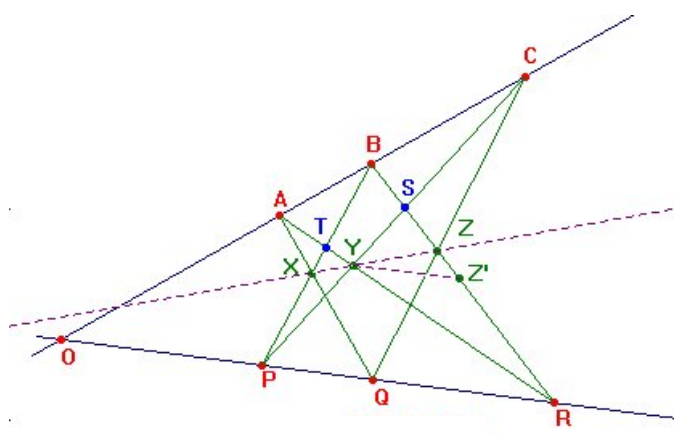
\includegraphics[scale = 0.30]{3.2_1}
\centering
\end{figure}

En los dos teoremas siguientes se darán dos versiones afines del teorema de Pappus, dependiendo de la recta que esté en el infinito.

\begin{theorem}
Sea $(A,B,C)$ una terna de puntos distintos de una recta $r$ del plano afín y sea $(P,Q,R)$ otra terna de puntos distintos sobre otra recta $s$ tal que $r \cap s \notin \{A,B,C\}$. Si $\overline{AQ}$ es paralela a $\overline{BP}$ y $\overline{AR}$ es paralela a $\overline{CP}$, entonces $\overline{BR}$ es paralela a $\overline{CQ}$.
\end{theorem}

\begin{proof}
No hay más que aplicar el teorema de Pappus en la envolvente proyectiva teniendo en cuenta que $\overline{XY}$ es la recta del infinito.
\end{proof}

\begin{figure}[h]
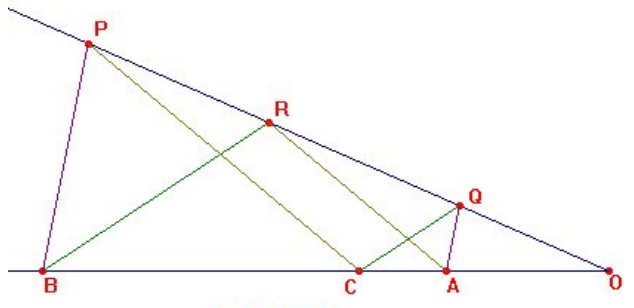
\includegraphics[scale = 0.30]{3.2_2}
\centering
\end{figure}

\begin{theorem}[Teorema menor de Pappus]
Sean $A,B,C$ puntos de una recta $r$ de un plano afín y $P,Q,R$ otros tres puntos sobre una recta $s$ del mismo plano paralela a $r$. Si $\overline{AQ}$ es paralela a $\overline{BP}$ y $\overline{AR}$ es paralela a $\overline{CP}$, entonces $\overline{BR}$ es paralela a $\overline{CQ}$.
\end{theorem}
\begin{proof}
Es el mismo teorema de antes pero con $r \cap s$ en el infinito.
\end{proof}

\begin{figure}[h]
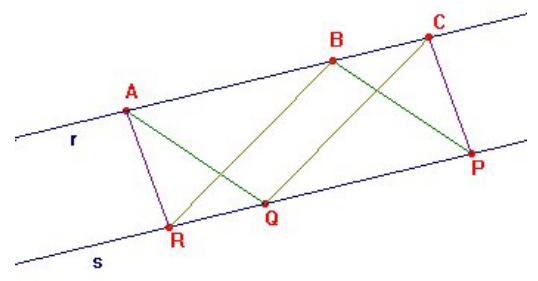
\includegraphics[scale = 0.35]{3.2_3}
\centering
\end{figure}

\section{Teorema de Desargues}

\begin{definition}
Tres puntos $A,B,C$ de un plano proyectivo no alineados se dirá que forman un \ul{triángulo}, y se denotará $ABC$.
\end{definition}

\begin{theorem}[Teorema de Desargues]
Sean $ABC$ y $A'B'C'$ dos triángulos de un plano proyectivo tales que las rectas $\overline{AA'}, \overline{BB'}$ y $\overline{CC'}$ intersecan en un punto $O$. Entonces los puntos $P = \overline{AB} \cap \overline{A'B'}$, $Q = \overline{AC} \cap \overline{A'C'}$ y $R = \overline{BC} \cap \overline{B'C'}$ están alineados.
\end{theorem}

\begin{proof}
Se va a probar que $S = \overline{BC} \cap \overline{PQ} = R$. Sea $\sigma$ la homología de centro $O$ y eje $\overline{PQ}$ que transforma $A$ en $A'$. Entonces usando que $B = \overline{OB} \cap \overline{AP}$ y que $C = \overline{OC} \cap \overline{AQ}$ se demuestra
\[\sigma(B) = \overline{A'P} \cap \overline{OB} = B' \qquad \sigma(C) = \overline{A'Q} \cap \overline{OC} = C'\]
luego $\sigma(\overline{BC}) = \overline{B'C'}$. Como $S$ es doble (pues pertenece al eje de la homología), entonces $S = \sigma(S) = \overline{B'C'} \cap \overline{\sigma(P)\sigma(Q)} = \overline{B'C'} \cap \overline{PQ} = R$, luego $R \in \overline{PQ}$.
\end{proof}

\begin{figure}[h]
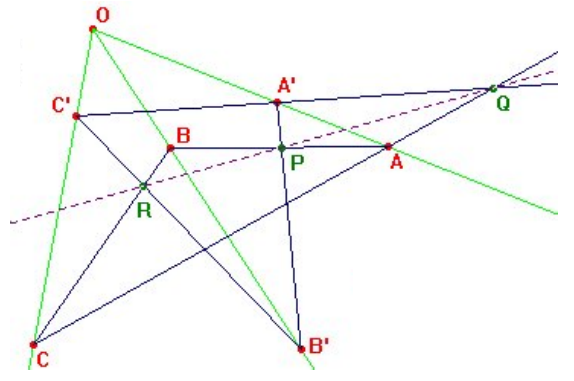
\includegraphics[scale = 0.4]{3.3_1}
\centering
\end{figure}

A partir del teorema de Desargues, el principio de dualidad proporciona dos teoremas gratis: el dual y el recíproco, que son exactamente iguales.

\begin{definition}
A dos triángulos de un plano en la configuración de la hipótesis del teorema de Desargues se les llama \ul{homólogos}.
\end{definition}

El motivo de esta denominación es que la homología $\sigma$ que aparece en la demostración hace $\sigma(A) = A', \sigma(B) = B'$ y $ \sigma(C)=C'$.

\chapter{Geometría ortogonal}

El objetivo de este tema no es más que establecer herramientas útiles para el posterior estudio de cónicas y cuádricas.

\section{Formas cuadráticas}

\begin{definition}
\label{def4.1.}
Una \ul{cónica} es un subconjunto $Q$ del plano afín $\mathbb{K}^2$ definido como el conjunto de ceros de un polinomio de segundo grado en dos variables:
\[Q = \{(x,y) \in \mathbb{K}^2 \colon a_{00}+2a_{01}x+2a_{02}y+a_{11}x^2+2a_{12}xy+a_{22}y^2=0\}\]
\end{definition}

El motivo de que aparezcan algunos doses en la ecuación anterior se razonará un poco más adelante.

\begin{example}
Algunas cónicas y sus ecuaciones:
\begin{itemize}
    \item Circunferencia: $(x-a)^2+(y-b)^2=r^2$.
    \item Elipse: $\frac{x^2}{a^2}+\frac{y^2}{b^2} =1$.
    \item Parábola: $y = ax^2+bx+c$.
    \item Hipérbola: $\frac{x^2}{a^2}-\frac{y^2}{b^2}=1$.
\end{itemize}
\end{example}

El objetivo es definir las cónicas en el espacio proyectivo de forma que al restringirlas al afín se obtenga lo que se ha definido ahora. Pasando a coordenadas homogéneas mediante $x = \frac{x_1}{x_0}, y = \frac{x_2}{x_0}$ en la ecuación de la cónica y multiplicando por $x_0^2$ para quitar denominadores,
\[a_{00}x_0^2+2a_{01}x_0x_1+2a_{02}x_0x_2+a_{11}x_1^2+2a_{12}x_1x_2+a_{22}x_2^2=0\]
Matricialmente,
\[
\begin{pmatrix*}[r]
x_0 & x_1 & x_2
\end{pmatrix*} \begin{pmatrix*}[r]
a_{00} & a_{01} & a_{02} \\
a_{01} & a_{11} & a_{12} \\
a_{02} & a_{12} & a_{22}
\end{pmatrix*} \begin{pmatrix*}[r]
    x_0 \\
    x_1 \\
    x_2
\end{pmatrix*} = 0
\]
lo que justifica la comodidad que supone colocar aquellos doses en la ecuación de la cónica.


\vspace{2mm}
Al estar trabajando con coordenadas homogéneas, serán de especial interés los polinomios como los siguientes:
\begin{definition}
Un polinomio $q$ en $n$ variables sobre un cuerpo $\mathbb{K}$ es \ul{homogéneo de segundo grado} si todos sus sumandos son de grado $2$, o equivalentemente, si para todo $\lambda \in \mathbb{K}$ se tiene
\[q(\lambda x_1,\mathellipsis,\lambda x_n) = \lambda^2q(x_1,\mathellipsis,x_n)\]
\end{definition}

Volviendo a la ecuación matricial de la página anterior, para el estudio de una cónica en el espacio proyectivo parece que será útil investigar las aplicaciones de la forma
\[
\begin{aligned}[t]
q \colon \mathbb{K}^3 \times \mathbb{K}^3 &\longrightarrow \mathbb{K} \\
(u,v) &\longmapsto q(u,v) = u^tAv
\end{aligned}
\]
donde $A$ es una cierta matriz simétrica. Esta función satisface las propiedades de bilinealidad y simetría. En efecto,
\begin{itemize}
    \item $q(\lambda_1 u_1+\lambda_2 u_2, v) = (\lambda_1 u_1+\lambda_2 u_2)Av_t = \lambda_1 u_1^t A v+\lambda_2u_2^tAv=\lambda_1 q(u_1,v)+\lambda_2 q(u_2,v)$
    \item Análogamente se demuestra la linealidad en el segundo argumento.
    \item $q(u,v) = u^tAv = (u^tAv)^t = v^tA^tu = v^tAu = q(v,u)$.
\end{itemize}
Todo esto motiva las siguientes definiciones:

\begin{definition}
Sea $V$ un espacio vectorial sobre $\mathbb{K}$. Un \ul{producto interno} es una aplicación $q \colon V \times V \to \mathbb{K}$ verificando
\begin{itemize}
    \item[(i)] $q(\lambda u+\mu v, w) = \lambda q(u,w)+\mu q(v,w)$
    \item[(ii)] $q(u, \lambda v + \mu w) = \lambda q(u,v)+\mu q(u,w)$
    \item[(iii)] $q(u,v) = q(v,u)$
\end{itemize}
para cualesquiera $u,v,w \in V, \lambda, \mu \in \mathbb{K}$.
\end{definition}

\begin{definition}
\label{def4.4.}
Sea $V$ un espacio vectorial sobre $\mathbb{K}$. Una aplicación $q \colon V \to \mathbb{K}$ se dice que es una \ul{forma cuadrática} cuando
\begin{itemize}
    \item[(i)] Para cada $\lambda \in \mathbb{K}$ y cada $u \in V$ se tiene $q(\lambda u) = \lambda^2 q(u)$.
    \item[(ii)] La aplicación definida por
    \[q(u,v) = \frac{1}{2}(q(u+v)-q(u)-q(v))\]
    constituye un producto interno, que recibe el nombre de \ul{función polarizada} de $q$.
\end{itemize}
\end{definition}

Una forma cuadrática y su polarizada se representan por la misma letra. La distinción entre ambas quedará clara si se observa el número de argumentos de cada una.

\vspace{2mm}
De la misma forma que a partir de una forma cuadrática se obtiene un producto interno, dado un producto interno $q$, la aplicación definida por $q(u) = q(u,u)$ define una forma cuadrática. Además, su polarizada coincide con el producto interno inicial.

\begin{proposition}
En un espacio vectorial $V$ sobre $\mathbb{K}$, toda matriz simétrica $A$ define una forma cuadrática mediante $u \mapsto u^tAu$, cuya polarizada está dada por $(u,v) \mapsto u^tAv$. Es más, todas las formas cuadráticas proceden de una matriz simétrica.  
\end{proposition}
\begin{proof}
Solo se va a probar lo que afirma la segunda oración. Sea $\mathcal{B} = \{u_1,\mathellipsis,u_n\}$ una base de un espacio vectorial $V$ sobre el cuerpo $\mathbb{K}$ y sea $q$ una forma cuadrática. Basta conocer los valores de los productos internos $\alpha_{ij} = q(u_i,u_j)$ para determinar cualquier otro producto interno $q(u,v)$. En efecto, si $u = x_1u_1+\mathellipsis+x_nu_n$, $v = y_1 u_1+\mathellipsis+y_n u_n$ son vectores cualesquiera, entonces
\[q(u,v) = q(x_1u_1+\mathellipsis+x_nu_n,y_1 u_1+\mathellipsis+y_n u_n) = \sum_{i=1}^n\sum_{j=1}^nx_iy_jq(u_i,u_j) = \sum_{i=1}^n\sum_{j=1}^nx_iy_j\alpha_{ij}\]
lo que matricialmente se escribe como
\[q(u,v)= \begin{pmatrix*}[r]
    x_1 & x_2 & \mathellipsis & x_n
\end{pmatrix*} \begin{pmatrix*}
    \alpha_{11} & \alpha_{12} & \mathellipsis & \alpha_{1n} \\
    \alpha_{12} & \alpha_{22} & \mathellipsis & \alpha_{2n} \\
    \vdots & \vdots & \ddots & \vdots \\
    \alpha_{1n} & \alpha_{2n} & \mathellipsis & \alpha_{nn}
\end{pmatrix*} \begin{pmatrix*}
    y_1 \\
    y_2 \\
    \vdots \\
    y_n
\end{pmatrix*} = x^tAy\]
donde la simetría de la matriz $A$ viene de $\alpha_{ij} = q(u_i,u_j) = q(u_j,u_i) = \alpha_{ij}$.
\end{proof}

Evidentemente, la ecuación anterior depende de la base del espacio vectorial tomada. Si $A$ y $B$ son las matrices de la misma forma cuadrática respecto de distintas bases y $P$ es la matriz del cambio de base (que es ortogonal por ser $A$, $B$ simétricas), entonces se tiene que $A = P^tBP$.

\section{Ortogonalidad}

\begin{definition}
Dado un espacio vectorial $V$ provisto de una forma cuadrática $q$, se dice que dos vectores $u, v$ son \ul{ortogonales} si $q(u,v)=0$. Un vector ortogonal a sí mismo se dice que es \ul{isótropo}.
\end{definition}

\begin{definition}
Dado un subespacio $S$ de un espacio vectorial $V$ provisto de una forma cuadrática $q$, se dice que $S$ es \ul{totalmente isotrópico} si está formado por vectores isótropos. Si el único vector isótropo es el cero, se dirá que $S$ es \ul{no isotrópico}. El \ul{ortogonal} de $S$ se define como
\[S^\perp = \{v \in V \colon q(v,s) = 0 \ \forall \ s \in S\}\]
\end{definition}

\begin{definition}
Dado un espacio vectorial $V$ provisto de una forma cuadrática $q$, se define el \ul{radical} de $V$ como
\[\textrm{Rad}(V) = \{u \in V \colon q(u,v)=0 \ \forall \ v \in V\}\]
Si $\textrm{Rad}(V)$ contiene otros vectores además del cero, se dirá que $V$ y $q$ son \ul{degenerados}. 

\vspace{2mm} Con la terminología establecida, se tiene $\textrm{Rad}(V)=V^\perp$. Además, si $S \leq V$, tiene sentido considerar la restricción de $q$ al espacio vectorial $S$, de forma que se puede definir
\[\textrm{Rad}(S) = \{u \in S \colon q(u,s)=0 \ \forall \ s \in S\} = S \cap S^\perp\]
\end{definition}

\begin{definition}
Dado un espacio vectorial $V$ provisto de una forma cuadrática $q$, una suma directa de subespacios $S_1 \oplus \mathellipsis \oplus S_n$ se dice que es una \ul{suma ortogonal-directa} si para cada $i \neq j$ se tiene $q(S_i,S_j) = 0$.
\end{definition}

\begin{theorem}
\label{teo4.1.}
Sea $q \colon V \to \mathbb{K}$ una forma cuadrática en el espacio vectorial $V$ sobre $\mathbb{K}$.
\begin{itemize}
    \item[(i)] Para cada subconjunto $S \subset V$, el ortogonal $S^\perp$ es un subespacio de $V$. En particular, $\textup{Rad}(V)$ es un subespacio de $V$.
    \item[(ii)] Si $S,T \subset V$, entonces $S \subset T$ implica $T^\perp \subset S^\perp$.
    \item[(iii)] Si $S \leq V$ es tal que $V = \textup{Rad}(V) \oplus S$, entonces $S$ es no degenerado.
    \item[(iv)] Si $A$ es la matriz de $q$ respecto de cualquier base, entonces 
    \[\textup{dim}(V) = \textup{dim}(\textup{Rad}(V))+\textup{rg}(A)\]
    En consecuencia, $q$ es no degenerada si y solo si $A$ es inversible.
    \item[(v)] Si $V$ es totalmente isotrópico, entonces $q(u,v) = 0 \ \forall \ u,v \in V$ y respecto de cualquier base, la matriz de $q$ es la matriz nula.
    \item[(vi)] Si un subespacio es no isotrópico, entonces es no degenerado.
\end{itemize}
\end{theorem}

\begin{proof}
Solo se va a demostrar $(iv)$ porque el procedimiento de la demostración será útil en la práctica para encontrar el radical. Sea
\[A = \begin{pmatrix*}
    \alpha_{11} & \alpha_{12} & \mathellipsis & \alpha_{1n} \\
    \alpha_{12} & \alpha_{22} & \mathellipsis & \alpha_{2n} \\
    \vdots & \vdots & \ddots & \vdots \\
    \alpha_{1n} & \alpha_{2n} & \mathellipsis & \alpha_{nn}
\end{pmatrix*}\]
la matriz de $q$ respecto de cierta base $\mathcal{B} = \{u_1,\mathellipsis,u_n\}$. Si $v \in V$, entonces $v \in \textrm{Rad}(V)$ si y solo si $q(u_i,v) = 0$ para cada $i = 1,\mathellipsis,n$. Si $v = x_1u_1+\mathellipsis+x_nu_n$, las condiciones $q(u_i,v) = 0$ se escriben como
\[0 = q(u_i,x_1u_1+\mathellipsis+x_nu_n) = x_1q(u_i,u_1)+\mathellipsis+x_nq(u_i,u_n) = \sum_{j=1}^n\alpha_{ij}x_j\]
lo que da lugar a un sistema de $n$ ecuaciones con $n$ incógnitas,
\[
\begin{cases}
    \alpha_{11}x_1+\alpha_{12}x_2+\mathellipsis+\alpha_{1n}x_n = 0 \\
    \alpha_{21}x_1+\alpha_{22}x_2+\mathellipsis+\alpha_{2n}x_n = 0\\
    \ \ \ \vdots \\
    \alpha_{n1}x_1+\alpha_{n2}x_2+\mathellipsis+\alpha_{nn}x_n = 0\\
\end{cases}
\]
cuya matriz de coeficientes es $A$ y cuyo espacio de soluciones es $\textrm{Rad}(V)$. El hecho de que la dimensión del espacio de soluciones sea la diferencia entre el número de incógnitas y el rango de la matriz de coeficientes termina la demostración.
\end{proof}

Respecto a este teorema, del último apartado se dirá que el recíproco es falso, como se comprobará en el ejemplo que sigue. La no isotropía no solo es una propiedad más fuerte que la no degeneración, sino que además la primera se hereda por subespacios y la segunda no.

\begin{example}
En $V = \R^3$, considérese la forma cuadrática cuya matriz respecto de la base canónica es
\[A = \begin{pmatrix*}[r]
    0 & -1 & 0 \\
    -1 & -\frac{1}{2} & 0 \\
    0 & 0 & 3
\end{pmatrix*}\]
Como $\textrm{det}(A) \neq 0$, entonces $q$ no degenera en $V$. Sin embargo, el subespacio generado por $(1,0,0)$ sí degenera, y además es totalmente isotrópico.

\end{example}

\begin{example}
En $V = \R^3$, considérese la forma cuadrática $q \colon \R^3 \to \R$ dada por
\[q(x_1,x_2,x_3) = x_1^2+2x_1x_3+2x_2^2+4x_2x_3+3x_3^2\]
Respecto de la base canónica de $\R^3$, la matriz de $q$ es
\[A = \begin{pmatrix*}[r]
    1 & 0 & 1 \\
    0 & 2 & 2 \\
    1 & 2 & 3
\end{pmatrix*}\]

\vspace{2mm}
\noindent De los dos ceros que hay en la matriz se deduce que los vectores $e_1 = (1,0,0)$ y $e_2 = (0,1,0)$ son ortogonales. Un vector isótropo, es, por ejemplo, $w = (1,1,-1)$, pues $q(w,w) = 0$. Por tanto, $W = \ < w>$ es totalmente isótropico.

\vspace{2mm}
\noindent Ahora se va a calcular el radical de $V$ siguiendo el esquema de la demostración anterior. Se tiene que $(x_1,x_2,x_3) \in \textrm{Rad}(V)$ si y solo si
\begin{itemize}
    \item $ \displaystyle
\begin{pmatrix*}[r]
    1 & 0 & 0
\end{pmatrix*}\begin{pmatrix*}[r]
    1 & 0 & 1 \\
    0 & 2 & 2 \\
    1 & 2 & 3
\end{pmatrix*}\begin{pmatrix*}[r]
    x_1 \\
    x_2 \\
    x_3
\end{pmatrix*} = 0 \iff \begin{cases}
    x_1+x_3=0
\end{cases}
$
    \item $ \displaystyle
\begin{pmatrix*}[r]
    0 & 1 & 0
\end{pmatrix*}\begin{pmatrix*}[r]
    1 & 0 & 1 \\
    0 & 2 & 2 \\
    1 & 2 & 3
\end{pmatrix*}\begin{pmatrix*}[r]
    x_1 \\
    x_2 \\
    x_3
\end{pmatrix*} = 0 \iff \begin{cases}
    2x_2+2x_3=0
\end{cases}
$
    \item $ \displaystyle
\begin{pmatrix*}[r]
    0 & 0 & 1
\end{pmatrix*}\begin{pmatrix*}[r]
    1 & 0 & 1 \\
    0 & 2 & 2 \\
    1 & 2 & 3
\end{pmatrix*}\begin{pmatrix*}[r]
    x_1 \\
    x_2 \\
    x_3
\end{pmatrix*} = 0 \iff \begin{cases}
    x_1+2x_2+3x_3=0
\end{cases}
$
\end{itemize}
La resolución del correspondiente sistema da $\textrm{Rad}(V) = \ < (1,1,-1)>$, así que $V$ junto con $q$ es degenerado.

\vspace{2mm}
\noindent Por último, se va a dar un ejemplo de suma ortogonal-directa. Considérense los subespacios $S = \ <(1,1,-1)>$, $T = \ <(1,0,1),(0,0,1)>$. Entonces
\begin{itemize}
    \item $ S^\perp = \{(x_1,x_2,x_3) \in \R^3 \colon \begin{pmatrix*}[r]
    x_1 & x_2 & x_3
\end{pmatrix*} A \begin{pmatrix*}[r]
    1 \\
    1 \\
    -1
\end{pmatrix*} = 0\} = V$
    \item $\begin{aligned}[t] T^\perp &= \{(x_1,x_2,x_3) \in \R^3 \colon \begin{pmatrix*}[r]
    x_1 & x_2 & x_3
\end{pmatrix*}A\begin{pmatrix*}[r]
    1 \\
    0 \\
    1
\end{pmatrix*} = 0, \begin{pmatrix*}[r]
    x_1 & x_2 & x_3
\end{pmatrix*}A\begin{pmatrix*}[r]
    0 \\
    0 \\
    1
\end{pmatrix*} = 0\}
    \end{aligned}$
\end{itemize}
Las ecuaciones cartesianas de $T^\perp$ son
\[
T^\perp \equiv \spalignsys{
    2x_1+2x_2+4x_3=0 ;
    x_1+2x_2+3x_3=0
}
\]
que dan como solución $T^\perp = S$. Por tanto, se tiene $q(S,T) = 0$, de donde se deduce que la suma $V = S \oplus T$ es ortogonal-directa.
\end{example}

\begin{proposition}
\label{prop4.1.}
Para cualquier subespacio $S$ de un espacio vectorial $V$ con una forma cuadrática, se tiene
\[\textup{dim}(S^\perp) = \textup{dim}(V) - \textup{dim}(S) + \textup{dim}(S \cap \textup{Rad}(V))\]
\end{proposition}

\begin{proof}
Ejercicio.
\end{proof}

\begin{proposition}
Para cualquier subespacio $S$ de un espacio vectorial $V$ no degenerado, se tiene
\[(S^\perp)^\perp = S\]
\end{proposition}

\begin{proof}
Consecuencia directa de la proposición anterior.
\end{proof}

\begin{theorem}[Teorema del sumando directo]
Sea $V$ un espacio vectorial sobre $\mathbb{K}$ con un producto interno $q$ y sea $S$ un subespacio de $V$ no degenerado. Entonces $V = S \oplus S^\perp$.
\end{theorem}

\begin{proof}
Consecuencia directa de la \hyperref[prop4.1.]{\color{blue}Proposición 4.2}.
\end{proof}

En la situación descrita en el teorema anterior, a $S^\perp$ se le llama \ul{complemento ortogonal} de $S$.

\begin{theorem}[Teorema de diagonalización]
\label{teo4.3.}
Todo espacio vectorial $V$ provisto de una forma cuadrática $q$ posee una base ortogonal.
\end{theorem}

\begin{proof}
Sea $u_1$ un vector no isótropo de $V$. Si no existiese tal vector, la parte $(iv)$ del \hyperref[teo4.1.]{\color{blue}Teorema 4.1} diría que cualquier pareja de vectores de $V$ es ortogonal, luego toda base es ortogonal y el teorema estaría demostrado. En caso contrario, como se tiene que $V_1 = \ <u_1>$ es no isótropo, entonces no degenera y el teorema del sumando directo permite escribir $V = V_1 \oplus V_1^\perp$.

\vspace{2mm}
Ahora se argumenta de la misma manera con $V_1^\perp$: si no hubiese ningún vector no isótropo, se completa $u_1$ con cualquier base de $V_1^\perp$ para obtener una base ortogonal de $V$. En otro caso, se elige $u_2 \in V_1^\perp$ con $q(u_2) \neq 0$. La matriz de $q$ restringida a $V_2 = \ <u_1,u_2>$ sería
\[A = \begin{pmatrix*}[r]
    q(u_1) & 0 \\
    0 & q(u_2)
\end{pmatrix*}\]
y como $\textrm{det}(A) = q(u_1)q(u_2) \neq 0$, entonces $V_2$ tampoco degenera y el teorema del sumando directo dice que $V = V_2 \oplus V_2^\perp$.

\vspace{2mm}
Una vez más: si $V_2^\perp$ es totalmente isotrópico la demostración se termina completando $\{u_1,u_2\}$ con una base de $V_2^\perp$, y si por contrario existiese $u_3 \in V_2^\perp$ con $q(u_3) \neq 0$, el subespacio $V_3 = \ <u_1,u_2,u_3>$ satisfaría $V = V_3 \oplus V_3^\perp$ y además la matriz de $q$ restringida a $V_3$ sería
\[B = \begin{pmatrix*}[r]
    q(u_1) & 0 & 0 \\
    0 & q(u_2) & 0 \\
    0 & 0 & q(u_3)
\end{pmatrix*}\]
El hecho de que cada $V_i^\perp$ reduzca en $1$ su dimensión con respecto al anterior junto con que $V$ tiene dimensión finita obliga a que el problema se acabe en algún momento, perdurando, a lo sumo, $\textrm{dim}(V) = n$ pasos. Así, o bien algún $V_i^\perp$ es totalmente isotrópico (lo que significaría $\textrm{Rad}(V) = V_i^\perp$), o bien $V_n^\perp = 0$ y $\{u_1,u_2,\mathellipsis,u_n\}$ es la base ortogonal deseada.
\end{proof}

\begin{example}
En $V = \R^4$, se considera la forma cuadrática dada por
\[q(x_1,x_2,x_3,x_4) = 2x_1x_2-2x_1x_3+x_2^2+4x_2x_4-2x_3^2+2x_3x_4\]
Se construirá una base ortogonal $\{u_1,u_2,u_3,u_4\}$ en este espacio razonando como en la demostración del teorema. La matriz de $q$ respecto de la canónica es
\[A = \begin{pmatrix*}[r]
    0 & 1 & -1 & 0 \\
    1 & 1 & 0 & 2 \\
    -1 & 0 & -2 & 1 \\
    0 & 2 & 1 & 0
\end{pmatrix*}\]
Primero se elige un vector no isótropo, por ejemplo $u_1 = e_2$, y se calcula el complemento ortogonal de $V_1 = \ < u_1>$ imponiendo
\[\begin{pmatrix*}[r]
    0 & 1 & 0 & 0
\end{pmatrix*} \begin{pmatrix*}[r]
    0 & 1 & -1 & 0 \\
    1 & 1 & 0 & 2 \\
    -1 & 0 & -2 & 1 \\
    0 & 2 & 1 & 0
\end{pmatrix*} \begin{pmatrix*}[r]
    x_1 \\
    x_2 \\
    x_3 \\
    x_4
\end{pmatrix*} = 0
 \]
 lo que proporciona la ecuación
 \[V_1^\perp \equiv \begin{cases}
     x_1+x_2+2x_4=0
 \end{cases}\]
Ahora se escoge un vector no isótropo de $V_1^\perp$. Se podría caracterizar mediante una ecuación a los vectores isótropos de $V_1^\perp$ y elegir alguno que no la cumpla, o también se podría ver a simple vista que $u_2 = e_3$ verifica la ecuación de $V_1^\perp$ y $q(u_2)=-2\neq 0$. Considerando $V_2 = \ <u_1,u_2>$, las ecuaciones del complemento ortogonal son
\[ V_2^\perp \equiv
\spalignsys{
x_1 + x_2 \. \+ + 2x_4 = 0 ;
-x_1 \. \+ - 2x_3 + x_4 = 0
}
\]
es decir, $V_2^\perp = \ <(-2,2,1,0),(1,-3,0,1)>$. El vector $u_3 = (1,-3,0,1) \in V_2^\perp$ satisface
\[q(u_3)= \begin{pmatrix*}[r]
    1 & -3 & 0 & 1
\end{pmatrix*}\begin{pmatrix*}[r]
    0 & 1 & -1 & 0 \\
    1 & 1 & 0 & 2 \\
    -1 & 0 & -2 & 1 \\
    0 & 2 & 1 & 0
\end{pmatrix*} \begin{pmatrix*}[r]
    1 \\
    -3 \\
    0 \\
    1
\end{pmatrix*} = 9 \neq 0\]
Haciendo más cuentas se llega a
\[V_3^\perp \equiv 
\spalignsys{
x_1 + x_2 \. \+ + 2x_4 = 0 ;
-x_1 \. \+ - 2x_3 + x_4 = 0 ;
-3x_1 \. \. \. \+ - 6x_4 = 0
}\]
donde $V_3 = \ <u_1,u_2,u_3>$. Por último, eligiendo el vector $u_4=(4,8,-3,2) \in V_3^\perp$, que verifica $q(u_4)=82 \neq 0$, se tiene que la matriz de $q$ en la base ortogonal $\{u_1,u_2,u_3,u_4\}$ es
\[B = \begin{pmatrix*}[r]
    1 & 0 & 0 & 0 \\
    0 & -2 & 0 & 0 \\
    0 & 0 & 9 & 0 \\
    0 & 0 & 0 & 82
\end{pmatrix*}\]
\end{example}

\section{Descomposición de Sylvester}

\begin{theorem}[Descomposición de Sylvester]
Sea $q \colon V \to \mathbb{K}$ una forma cuadrática del espacio vectorial $V$ sobre el cuerpo ordenado $\mathbb{K}$. Entonces existen subespacios $V_+, V_0$ y $V_-$ tales que
\begin{itemize}
    \item[(i)] $V$ se descompone en la suma ortogonal-directa 
    \[V = V_+ \oplus V_0 \oplus V_-\]
    \item[(ii)] La restricción de $q$ a $V_+$ es definida positiva, es decir, $q(u) > 0 \ \forall \ u \in V_+ \setminus \{0\}$.
    \item[(iii)] La restricción de $q$ a $V_-$ es definida negativa, es decir, $q(u) < 0 \ \forall \ u \in V_- \setminus \{0\}$.
    \item[(iv)] $V_0$ es totalmente isotrópico. Es más, $V_0 = \textup{Rad}(V)$.
\end{itemize}

Además, si $V = W_+ \oplus W_0 \oplus W_-$ es otra descomposición de $V$ en suma ortogonal-directa con $q$ definida positiva en $W_+$, definida negativa en $W_-$ e idénticamente nula en $W_0$, entonces $\textup{dim}(W_+) = \textup{dim}(V_+)$, $\textup{dim}(W_0) = \textup{dim}(V_0)$ y $\textup{dim}(W_-) = \textup{dim}(V_-)$.
\end{theorem}

\begin{proof}
Solo se va a probar la existencia. Por el teorema de diagonalización, existe una base ortogonal $\{u_1,u_2,\mathellipsis,u_n\}$ de $V$, de la que se reordenarán los vectores para que se tenga $q(u_i) > 0 \ \forall \ i = 1,\mathellipsis,k$, $q(u_i)=0 \ \forall \ i = k+1,\mathellipsis,m$ y $q(u_i) < 0 \ \forall \ i = m+1,\mathellipsis,n$. Sean $V_+ = \ <u_1,\mathellipsis,u_k>, V_0 = \ <u_{k+1},\mathellipsis,u_m>$ y $V_- = \ <u_{m+1},\mathellipsis,u_n>$. La ortogonalidad dos a dos de estos subespacios es consecuencia de que la base tomada es ortogonal. El resto de propiedades se prueban fácilmente.
\end{proof}

\section{Descomposición de Witt}

\begin{definition}
Un \ul{plano hiperbólico} es un espacio vectorial bidimensional provisto de un producto interno no degenerado y con al menos un vector isótropo no nulo.
\end{definition}

\begin{proposition}
\label{prop4.4.}
Para un espacio vectorial $V$ sobre el cuerpo $\mathbb{K}$ bidimensional y con una forma cuadrática no degenerada $q$, son equivalentes:
\begin{itemize}
    \item[(i)] $V$ es un plano hiperbólico.
    \item[(ii)] Existe un par de vectores $u,v$ que definen una base respecto de la cual la matriz del producto interno es
    \[\begin{pmatrix*}[r]
        0 & 1 \\
        1 & 0
    \end{pmatrix*}\]
    \item[(iii)] Existe una base respecto de la cual la matriz de $q$ es
    \[\begin{pmatrix*}[r]
        1 & 0 \\
        0 & -1
    \end{pmatrix*}
    \]
\end{itemize}
Además, todo plano hiperbólico contiene dos rectas totalmente isotrópicas.
\end{proposition}

\begin{proof}
Se probará primero que $(i) \implies (ii)$. Sea $u \neq 0$ un vector isótropo. Veamos que existen otros vectores isótropos no nulos a parte de los proporcionales a $u$. Sea $w$ un vector tal que $u$ y $w$ son linealmente independientes, formando la base $\{u,w\}$ de $V$ respecto de la cual la matriz de $q$ es
\[\begin{pmatrix*}
    0 & q(u,w) \\
    q(u,w) & q(w)
\end{pmatrix*}\]
Si fuese $q(w,w) = 0$ hemos triunfado. En caso contrario, el determinante de la matriz anterior debe ser no nulo, pues $q$ no degenera. Que sea $-q(u,w)^2 \neq 0$ permite sustituir $w$ por $w' =\frac{w}{q(u,w)}$, dando lugar a la matriz
\[\begin{pmatrix*}
    0 & 1 \\
    1 & q(w')
\end{pmatrix*}\]
respecto de $\{u,w'\}$. Ahora se va a buscar algún vector isótropo de coordenadas $(1,x)$ en la base $\{u,w'\}$ planteando la ecuación
\[\begin{pmatrix*}
    1 & x
\end{pmatrix*} \begin{pmatrix*}
    0 & 1 \\
    1 & q(w')
\end{pmatrix*} \begin{pmatrix*}
    1 \\
    x
\end{pmatrix*}=0
\]
lo que da como posibilidades $x = 0$ (el propio $u$) y $x = -\frac{2}{q(w')}$. Por tanto, $v = u -\frac{2}{q(w')}w'$ es isótropo y linealmente independiente de $u$. Respecto de la base $\{u,v\}$, la matriz de $q$ es la que se busca.

\vspace{2mm}
Se procederá con la demostración de $(ii) \implies (iii)$. Sean $u, v$ vectores que satisfacen $(ii)$ y considérese la base $\{u_1,u_2\}$, donde $u_1 = \frac{1}{2}(u+v)$ y $u_2=\frac{1}{2}(u-v)$. Entonces $q$ se expresa por medio de la matriz
\[A = \begin{pmatrix*}[r]
    1 & 0 \\
    0 & -1
\end{pmatrix*}\]

En cuanto a $(iii) \implies (i)$, si $\{u_1,u_2\}$ es una base respecto de la cual la matriz de $q$ es $A$, entonces $V$ no degenera (pues $\textrm{det}(A) = -1$) y contiene al vector isótropo no nulo $u_1+u_2$. Por tanto, $V$ es un plano hiperbólico.

\vspace{2mm}
Por último, si $(u,v)$ es un par hiperbólico, entonces las rectas generadas por $u$ y $v$ constituyen dos subespacios unidimensionales totalmente isotrópicos, lo que desmuestra la última afirmación del teorema.

\end{proof}

\begin{definition}
El par $(u,v)$ que se manifiesta en $(ii)$ del teorema anterior se denomina \ul{par hiperbólico}.
\end{definition}

Se verá en lo que sigue la relación entre plano hiperbólico y proyectividad hiperbólica entre rectas. Sea $\sigma \colon \mathcal{P}_1(\mathbb{K}) \to \mathcal{P}_1(\mathbb{K})$ una proyectividad hiperbólica de ecuación general 
\[\lambda x x'+\mu x +\nu x' + \zeta = 0\]
Los puntos dobles de $\sigma$ son las soluciones de
\[\lambda x^2+(\mu+\nu)x+\zeta = 0\]
Pasando a coordenadas homogéneas por medio de $x = \frac{x_1}{x_0}$ y multiplicando por $x_0^2$ se obtiene
\[\lambda x_1^2 +(\mu+\nu)x_1x_0 + \zeta x_0^2 = 0\]
de forma que los puntos dobles de $\sigma$ se pueden ver como vectores isótropos no nulos del espacio vectorial $\mathbb{K}^2$ junto la forma cuadrática 
\[
\begin{aligned}[t]
q \colon \mathbb{K}^2 &\longrightarrow \mathbb{K} \\
(x_0, x_1) &\longmapsto q(x_0,x_1) = \lambda x_1^2 +(\mu+\nu)x_1x_0 + \zeta x_0^2
\end{aligned}
\]
Como un plano hiperbólico consta de dos vectores linealmente independientes, un producto interno no degenerado y un vector isótropo no nulo, solo resta comprobar que $q$ no degenera. Ahora bien, la matriz
\[\begin{pmatrix*}
    \zeta & \frac{\mu+\nu}{2} \\
    \frac{\mu+\nu}{2} & \lambda
\end{pmatrix*}\]
de $q$ respecto de la base canónica tiene determinante $\lambda \zeta - \frac{(\mu+\nu)^2}{4}$, que no se anula por ser la proyectividad hiperbólica, así que $\mathbb{K}^2$ es un plano hiperbólico junto con $q$. Por último, las rectas totalmente isotrópicas que se mencionan al final del teorema anterior se interpretan como la pareja de puntos dobles de la proyectividad.

\begin{theorem}[Descomposición de Witt]
Sea $q \colon V \to \mathbb{K}$ una forma cuadrática. Entonces $V$ se descompone en la suma ortogonal-directa
\[V = \textup{Rad}(V) \, \oplus \, \biggr( \bigoplus_{i \in S}P_i \biggl) \, \oplus \, W\]
donde los $P_i$ son planos hiperbólicos y $W$ es un subespacio no isotrópico. Además, cualquier otra descomposición de este tipo conserva el número de planos hiperbólicos y la dimensión de $W$.
\end{theorem}

\begin{proof}
Una vez más, solo se demostrará la existencia. Sea $S$ un subespacio de $V$ tal que $ V = \textup{Rad}(V) \oplus S$. Por el apartado tercero del \hyperref[teo4.1.]{\color{blue}Teorema 4.1}, se tiene que $S$ no degenera, así que se puede suponer sin perder generalidad que $V$ no degenera.

\vspace{2mm}
Se presenta ahora la siguiente disyuntiva: si en $V$ no hubiese ningún vector isótropo no nulo, entonces el teorema estaría demostrado (el número de planos hiperbólicos sería $0$). En caso contrario, sea $u_1 \in V \setminus \{0\}$ con $q(u_1) = 0$. Como $V$ es no degenerado, existe algún $v_1 \in V$ con $q(u_1,v_1) \neq 0$, convirtiéndose $P_1 = \ <u_1,v_1>$ en plano hiperbólico. Por el teorema del sumando directo, se tiene que $V = P_1 \oplus V_1$, donde $V_1 = P_1^\perp$. Por tanto,
\[\textup{Rad}(V_1) = V_1 \cap V_1^\perp = P_1^\perp \cap (P_1^\perp)^\perp = P_1^\perp \cap P_1 = \textup{Rad}(P_1)=\{0\}\]
luego $V_1$ no degenera y se puede continuar con el mismo razonamiento: si en $V_1$ no hubiese vectores isótropos no nulos, la demostración se acaba (el número de planos hiperbólicos sería $1$ y $V_1$ es el $W$ del enunciado). En otro caso, se podrían elegir $u_2,v_2 \in V$ con $q(u_2) = 0$ y $q(u_2,v_2) \neq 0$, apareciendo el plano hiperbólico $P_2 = \ <u_2,v_2>$. Ahora se consideraría $V_2 = (P_1 \oplus P_2)^\perp$ y se razonaría como antes. 

\vspace{2mm}
Como la dimensión de $V$ es finita, la película tiene que acabarse en algún momento, ya sea por culpa de un complemento ortogonal no isótropo de una suma de planos hiperbólicos, o por llegar a una suma ortogonal-directa de $V$ en planos hiperbólicos.
\end{proof}

\begin{definition}
El cardinal del conjunto de índices $S$ de la descomposición de Witt se llama \ul{índice de Witt}.
\end{definition}

Una importante circunstancia que se va afirmar sin demostrarse es que en un cuerpo algebraicamente cerrado (que $\mathbb{C}$ se dé por aludido) el índice de Witt alcanza siempre el máximo valor posible.

\begin{example}
Se va a desarrollar el argumento de la demostración del teorema anterior en un ejemplo concreto. En $V= \R^4$, considérese la forma cuadrática de matriz
\[A = \begin{pmatrix*}[r]
    0 & 1 & -1 & 0 \\
    1 & 1 & 0 & 2 \\
    -1 & 0 & -1 & -2 \\
    0 & 2 & -2 & 1
\end{pmatrix*}\]
en la base canónica. El radical de $V$ es la solución del sistema planteado a partir de las condiciones $q((x_1,x_2,x_3,x_4),e_i) = 0$ para cada $i = 1,2,3,4$, que sería
\[
\spalignsys{
\. \+ x_2 - x_3 \. \+ = 0 ;
x_1 + x_2 \. \+ + 2x_4 = 0 ;
-x_1 \. \+ - x_3 - 2x_4 = 0 ;
\. \+ 2x_2 - 2x_3 + x_4 = 0
}
\]
Se tiene $\textrm{Rad}(V)= \ <(-1,1,1,0)>$. Para hallar un suplemento $S$ del radical, se escogen tres vectores linealmente independientes entre sí y linealmente independientes de $v = (-1,1,1,0)$, como $S = \ <e_2,e_3,e_4>$. Para encontrar los vectores isótropos de $S$, se plantea la ecuación
\[\begin{pmatrix*}[r]
    0 & x & y & z
\end{pmatrix*}\begin{pmatrix*}[r]
    0 & 1 & -1 & 0 \\
    1 & 1 & 0 & 2 \\
    -1 & 0 & -1 & -2 \\
    0 & 2 & -2 & 1
\end{pmatrix*} \begin{pmatrix*}[r]
    0 \\
    x \\
    y \\
    z
\end{pmatrix*} = 0\]
Se han de encontrar vectores $(0,x,y,z)$ no nulos tales que
\[x^2+4xz-y^2-4yz+z^2=0\]
como por ejemplo $u_1=(0,1,1,0)$. Ahora hay que encontrar un vector no ortogonal a $u_1$. El vector $e_3$ satisface $q(e_3,u_1) = -1$, así que se considera el plano hiperbólico $P = \ <u_1,e_3>$. Las dimensiones impiden que haya otro plano hiperbólico en la descomposición de Witt, así que lo que resta en la descomposición, que es $P^\perp \cap S$, actuará de subespacio no isotrópico. De las condiciones
\[q(u_1,(0,x,y,z)) = 0 \qquad q(e_3,(0,x,y,z))\]
resulta el sistema de ecuaciones
\[
\spalignsys{
x - y \. \+ = 0 ;
\. - y - 2z = 0
}
\]
cuya solución es $W = \ <(0,-2,-2,1)>$. Conclusión:
\[V = \textup{Rad}(V) \oplus P \oplus W\]
con los sumandos directos ortogonales dos a dos. El índice de Witt en este caso sería $1$.

\end{example}

\chapter{Cuádricas en el espacio proyectivo}

\section{Introducción}

El tema anterior se inició definiendo las cónicas y siguió con el estudio de las formas cuadráticas. A fin de generalizar el concepto de cónica, se introduce la siguiente definición:

\begin{definition}
\label{def5.1.}
Una \ul{cuádrica} en el espacio afín $\mathbb{K}^n$ es el conjunto de puntos cuyas coordenadas cartesianas $(y_1,\mathellipsis,y_n)$ satisfacen $p(y_1,\mathellipsis,y_n) = 0$ para un cierto polinomio $p$ de segundo grado en $n$ variables.
\end{definition}

Al igual que se hizo con las cónicas, pasando a coordenadas homogéneas por medio de $y_i = \frac{x_i}{x_0}$ y multiplicando por $x_0^2$, se obtiene un nuevo polinomio $q$ dado por
\[q(x_0,x_1,\mathellipsis,x_n) = x_0^2 \, p\biggr(\frac{x_1}{x_0},\mathellipsis,\frac{x_n}{x_0} \biggl)\]
que tiene una variable más y es homogéneo de segundo grado, pues para cada $\lambda \in \mathbb{K}$ se tiene
\[q(\lambda x_0,\lambda x_1,\mathellipsis, \lambda x_n) = (\lambda x_0)^2 \, p\biggr(\frac{\lambda x_1}{\lambda x_0},\mathellipsis,\frac{\lambda x_n}{\lambda x_0} \biggl) = \lambda^2 x_0^2 \, p\biggr(\frac{x_1}{x_0},\mathellipsis,\frac{x_n}{x_0} \biggl) = \lambda^2q(x_0,x_1,\mathellipsis,x_n)\]
luego parece que $q$ tendrá algo que ver con las formas cuadráticas. Además, dado un punto $P = \ <v>$ del espacio proyectivo $\mathcal{P}(V)$ con $v = (x_0,x_1,\mathellipsis,x_n)$, que $P$ esté en la cuádrica significa que $q(v) = 0$. Todo esto conduce a redefinir las cuádricas como sigue:

\begin{definition}
\label{def5.2.}
Dado un espacio vectorial $V$ sobre el cuerpo $\mathbb{K}$ acompañado de una forma cuadrática $q \colon V \to \mathbb{K}$, se define la \ul{cuádrica proyectiva} como el conjunto $\mathcal{Q}(q)$ de los puntos del espacio proyectivo $\mathcal{P}(V)$ engendrados por vectores isótropos no nulos de $q$. A una cuádrica en dimensión dos se le llamará \ul{cónica}.
\end{definition}

Dada una cuádrica $\mathcal{Q}(q)$, el \hyperref[teo4.3.]{\color{blue}Teorema 4.3} permite encontrar una matriz de $q$ que sea diagonal, de forma que la cuádrica quedaría descrita por la ecuación
\[\begin{pmatrix*}
    x_0 & x_1 & \mathellipsis & x_n
\end{pmatrix*}\begin{pmatrix*}
    \alpha_0 & 0 & \mathellipsis & 0 \\
    0 & \alpha_1 & \mathellipsis & 0 \\
    \vdots & \vdots & \ddots & \vdots \\
    0 & 0 & \mathellipsis & \alpha_n
\end{pmatrix*} \begin{pmatrix*}
    x_0 \\
    x_1 \\
    \vdots \\
    x_n
\end{pmatrix*} = 0 \iff
\alpha_0x_0^2+\alpha_1x_1^2+\mathellipsis+\alpha_nx_n^2 = 0
\]
Esta última ecuación es denominada \ul{ecuación reducida} de la cuádrica.

\vspace{2mm}
También se resalta el hecho de que formas cuadráticas distintas pueden dar lugar a cuádricas idénticas. Por ejemplo,

\begin{example}
En $\mathcal{P}_1(\R)$, se consideran las cuádricas determinadas por las ecuaciones
\[x_0^2+x_1^2=0 \qquad x_0^2 + 2x_1^2 =0\]
Ambas cuádricas describen el conjunto vacío pero proceden de formas cuadráticas diferentes.
\end{example} 

\begin{theorem}
\label{teo5.1.}
    Una proyectividad entre espacios proyectivos transforma una cuádrica en otra cuádrica.
\end{theorem}

\begin{proof}
Sea $\sigma = \mathcal{P}(f) \colon \mathcal{P}(V) \to \mathcal{P}(V')$ una proyectividad entre espacios proyectivos de la misma dimensión sobre $\mathbb{K}$ y sea $\mathcal{Q}(q)$ una cuádrica en $\mathcal{P}(V)$. Considérese la composición $q' = q \circ f^{-1} \colon V' \to \mathbb{K}$, que es una forma cuadrática, pues si $\lambda \in \mathbb{K}$ y $v \in V'$, entonces
\[q'(\lambda v) = q(f^{-1}(\lambda v)) = q(\lambda f^{-1}(v)) = \lambda^2 q(f^{-1}(v)) = \lambda^2 q'(v)\]
Un razonamiento tan sencillo como este probaría que la polarizada de $q$ define un producto interno.

\vspace{2mm}
Veamos que $\sigma(\mathcal{Q}(q)) = \mathcal{Q}(q')$, lo que terminará la demostración. Si $P = \ < v>$ es un punto de $\mathcal{Q}(q)$, entonces
\[q'(f(v)) = q(f^{-1}(f(v))) = q(v) = 0\]
lo que significa que $f(v)$ (que es no nulo) es isótropo para $q'$, es decir, $\sigma(P) = \ < f(v)>$ es un punto de la cuádrica $Q(q')$. Por otro lado, si $P' = \ < u >$ está en $\mathcal{Q}(q')$, entonces
\[0 = q'(u) = q(f^{-1}(u))\]
así que $P' = \sigma(P)$, donde $P = \ < f^{-1}(u) >$ es un punto de $\mathcal{Q}(q)$. Por tanto, $P' \in \sigma(\mathcal{Q}(q))$.
\end{proof}

\section{Estudio de las cuádricas en dimensiones pequeñas}

Con dimensiones pequeñas se entiende a dimensiones menores que $2$. El estudio de las cuádricas de dimensión $2$ tendrá lugar más adelante.

\begin{itemize}
    \item En un espacio proyectivo de dimensión $-1$ toda cuádrica es vacía, pues el propio espacio proyectivo lo es.
    \item En un espacio proyectivo de dimensión $0$, toda cuádrica es el total o el vacío, pues solo hay un punto en el espacio proyectivo.
    \item En un espacio proyectivo de dimensión $1$, sea $\mathcal{Q}(q)$ una cuádrica de ecuación reducida
    \[\alpha_0x_0^2+\alpha_1x_1^2 = 0\]
    Se distinguen tres casos:
    \begin{itemize}
        \item[(i)] El rango de $q$ es 2. Como la matriz de $q$ es
        \[\begin{pmatrix*}
            \alpha_0 & 0 \\
            0 & \alpha_1
        \end{pmatrix*}\]
        entonces se tiene que $0 \notin \{\alpha_0, \alpha_1\}$, y por tanto la ecuación reducida se puede escribir como
        \[\biggl( \frac{x_1}{x_0} \biggr)^2 = -\frac{\alpha_0}{\alpha_1}\]
        ecuación que puede tener o no solución dependiendo del cuerpo $\mathbb{K}$. Si existe $\lambda \in \mathbb{K}$ tal que $\lambda^2 = -\frac{\alpha_0}{\alpha_1}$, entonces los puntos de $\mathcal{Q}(q)$ son aquellos que tienen coordenadas $(1, \lambda)$ y $(1, - \lambda)$. Si no existe un tal $\lambda \in \mathbb{K}$, entonces no hay puntos en la cuádrica.
        \item[(ii)] El rango de $q$ es 1. Esto significa que $\alpha_0 = 0$ ó $\alpha_1 = 0$ (nunca ambos a la vez). En el primer caso, la ecuación es $\alpha_1x_1^2 = 0$, lo que determina un único punto, el $(1,0)$. En el segundo caso, el único punto de la cuádrica sería el de coordenadas homogéneas $(0,1)$.
        \item[(iii)] El rango de $q$ es 0. Entonces $\alpha_0 = \alpha_1 = 0$ y todo punto cumple la ecuación de la cuádrica.
    \end{itemize}
    Conclusión: si la forma cuadrática no degenera, toda cuádrica consta de dos puntos o de ninguno, y si degenera, una cuádrica o tiene un único punto o los tiene todos.
\end{itemize}

\section{Posición relativa de una cuádrica y una recta}
\label{sec5.3.}

\begin{proposition}
    Sea $\mathcal{P}(S)$ un subespacio proyectivo de $\mathcal{P}(V)$ y sea $\mathcal{Q}(q)$ una cuádrica en $\mathcal{P}(V)$. Entonces $\mathcal{Q}(\bigl.q\bigr|_S)$ es una cuádrica de $\mathcal{P}(S)$ y además $\mathcal{Q}(\bigl.q\bigr|_S) = \mathcal{Q}(q) \cap \mathcal{P}(S)$.
\end{proposition}
\begin{proof}
Inmediata.
\end{proof}

A partir de ahora se escribirá $\mathcal{Q}(\bigl.q\bigr|_S) = \mathcal{Q}(q_S)$. En caso de que $r = \mathcal{P}(S)$ sea una recta, en la sección anterior se vio que si $q_S$ no degenera, entonces $\mathcal{Q}(q_S)$ tiene dos puntos o ninguno, es decir, $r$ corta a $\mathcal{Q}(q)$ en dos puntos o ninguno. 

\vspace{2mm}
En el primer caso se dice que la recta es \ul{secante} a la cuádrica y en el segundo caso, \ul{exterior} a la cuádrica. Si $q_S$ degenera, entonces la recta corta a la cuádrica en un punto o en todos y se dirá que la recta es \ul{tangente} a la cuádrica. Esto último es susceptible de generalizarse a subespacios de cualquier dimensión:

\begin{definition}
 Un subespacio $\mathcal{P}(S)$ del espacio proyectivo $\mathcal{P}(V)$ es \ul{tangente} a la cuádrica $\mathcal{Q}(q)$ si la restricción $q_S$ degenera.
\end{definition}

El hecho de que una cuádrica degenerada $\mathcal{Q}(q)$ en un espacio proyectivo $\mathcal{P}(V)$ contenga a todos los puntos $P = \ <v>$ con $v \in \textrm{Rad}(V)$ motiva la siguiente definición:

\begin{definition}
\label{def5.4.}
Dada una cuádrica $\mathcal{Q}(q)$ degenerada en un espacio proyectivo $\mathcal{P}(V)$, al subespacio $\mathcal{P}(\textrm{Rad}(V))$ se le denomina \ul{vértice} de la cuádrica, y cualquiera de sus puntos se dice que es \ul{singular}.
\end{definition}

\begin{definition}
Si $V$ es un espacio vectorial provisto de una forma cuadrática $q$ y se escribe $V = \textrm{Rad}(V) \, \oplus \, S$ con $S$ un subespacio no degenerado, entonces la cuádrica $\mathcal{Q}(q_S)$ del subespacio proyectivo $\mathcal{P}(S)$ se denomina \ul{directriz}.
\end{definition}

Nótese que una cuádrica puede tener varias directrices distintas, mientras que vértice hay uno solo.

\begin{definition}
Una recta que contenga puntos del vértice y de la directriz de una cuádrica se llamará \ul{generatriz}.
\end{definition}

\begin{figure}[h]
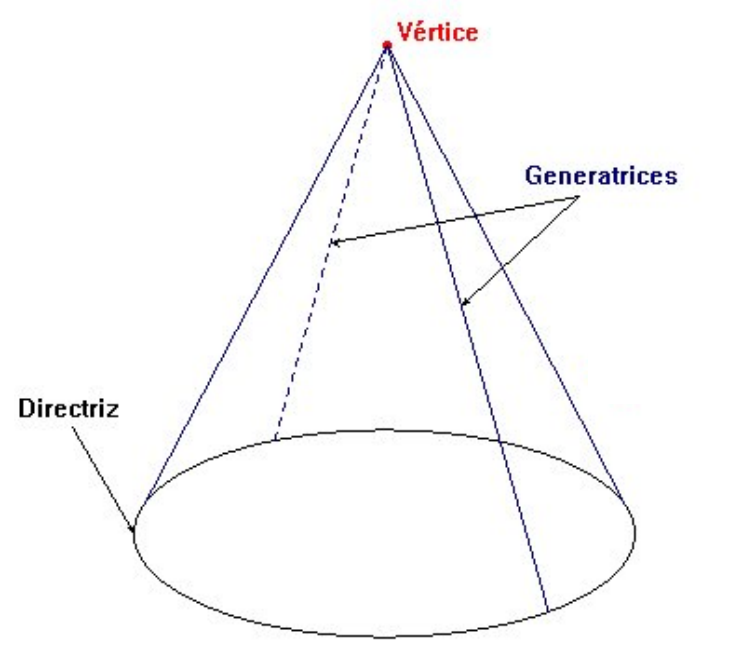
\includegraphics[scale = 0.27]{5.3_1}
\centering
\end{figure}

\begin{theorem}
\label{teo5.2.}
Si una cuádrica degenerada no se reduce al vértice, entonces se compone de rectas que pasan por puntos del vértice y de una directriz.
\end{theorem}

\begin{proof}
Sea $V$ un espacio vectorial sobre $\mathbb{K}$ dotado de una forma cuadrática $q$ y escríbase $V = \textrm{Rad(V)} \oplus S$. Sea $P = \ <u>$ un punto singular y $Q = \ <v>$ un punto de la directriz $\mathcal{Q}(q_S)$. Se va a comprobar que todo punto $R = \ <\alpha u + \beta v>$ de la recta $\overline{PQ}$ está en $\mathcal{Q}(q)$. Se tiene que
\[q(\alpha u + \beta v) = \alpha^2 q(u)+\beta^2 q(v) + 2\alpha \beta q(u,v) = 0\]
ya que $u \in \textrm{Rad}(V)$ y $v$ es isótropo. 

\vspace{2mm}
Recíprocamente, si $A = \ <a >$ es un punto de la cuádrica $\mathcal{Q}(q)$, la descomposición $V = \textrm{Rad}(V) \oplus S$ dice que existen vectores únicos $b \in \textrm{Rad}(V), \, c \in S$ tales que $a = b + c$. Ahora bien, por ser $a$ isótropo, se tiene
\[0 = q(a) = q(b+c) = q(b) + q(c) + 2q(b,c) = q(c)\]
Si $c = 0$, entonces $A = \ < a > \ = \ < b >$ sería un punto del vértice, y por tanto estaría en cualquier recta que pase por el vértice y por un punto de la directriz. Si $c \neq 0$, entonces $C = \ < c >$ está en la directriz $\mathcal{Q}(q_S)$, luego $A = \ <b+c> \ \in \overline{BC}$, que es una recta que pasa por un punto $B = \ <b>$ del vértice y un punto $C = \ < c >$ de la directriz $\mathcal{Q}(q_S)$.
\end{proof}

\begin{example}
Considérese la cónica $\mathcal{Q}(q)$ del plano proyectivo real descrita por la ecuación $x_1^2-x_2^2 = 0$. La matriz de $q$ en la base canónica sería
\[
\begin{pmatrix*}[r]
    0 & 0 & 0 \\
    0 & 1 & 0 \\
    0 & 0 & -1
\end{pmatrix*}
\]
Se tiene que $V = \textrm{Rad}(V) \oplus S$, donde $\textrm{Rad}(V) = \ < e_0 >$ y $S = <e_1, e_2>$, así que el vértice consta de un solo punto, $P = \ <e_0>$. Se procede a calcular la directriz $\mathcal{Q}(q_S) = \mathcal{Q}(q) \, \cap \, \mathcal{P}(S)$. Se tiene que
\[<(x_0,x_1,x_2)> \ \in \mathcal{P}(S) \iff \begin{vmatrix*}
    x_0 & x_1 & x_2 \\
    0 & 1 & 0 \\
    0 & 0 & 1
\end{vmatrix*} = 0 \iff x_0 = 0\]
luego $\mathcal{Q}(q_S)$ está formada por los puntos cuyos generadores satisfacen $x_1^2-x_2^2 = 0$ (o lo que es lo mismo, $x_1 = \pm \ x_2$) y $x_0 = 0$. La directriz sería entonces $\mathcal{Q}(q_S) = \{A,B\}$, donde $A = \ <(0,1,1)>, B = \ <(0,1,-1)>$. Si en lugar del complemento anterior se tomase por ejemplo $S = \ <(1,1,0),(1,0,1)>$, la directriz estaría compuesta por los puntos de coordenadas homogéneas $(2,1,1)$ y $(0,1,-1)$. 

\vspace{2mm}
\noindent Por último, el teorema anterior dice que la cónica se compone de las rectas $\overline{PA}$ y $\overline{PB}$. En efecto, de las condiciones
\[\begin{vmatrix*}
        x_0 & x_1 & x_2 \\
        1 & 0 & 0 \\
        0 & 1 & 1
    \end{vmatrix*} = 0 \iff x_1 = x_2 \qquad \qquad
\begin{vmatrix*}
        x_0 & x_1 & x_2 \\
        1 & 0 & 0 \\
        0 & 1 & -1
    \end{vmatrix*} = 0 \iff x_1 = -x_2\]
se deduce que la unión de las rectas tiene como ecuación $x_1 = \pm \ x_2$, es decir, $x_1^2 - x_2^2 = 0$, que es precisamente la ecuación de la cónica.
\end{example}

\begin{theorem}
\label{teo5.3.}
Un punto está en el vértice de una cuádrica si y solo si pertenece a la cuádrica y cada recta que pase por él es tangente a la cuádrica.
\end{theorem}

\begin{proof}
\hfill
\begin{itemize}
    \item[{\fbox[rb]{$\Rightarrow$}}] Sea $P = \ <u>$ un punto en el vértice de una cuádrica $\mathcal{Q}(q)$ de un espacio proyectivo $\mathcal{P}(V)$. Sea $\overline{PQ}$ una recta que pase por $P$, con $Q = \ <v>$. La matriz de $q$ restringida a $<u,v>$ en la base $\{u,v\}$ es
    \[\begin{pmatrix*}
        0 & 0 \\
        0 & q(v)
    \end{pmatrix*}\]
    luego dicha restricción degenera y por tanto la recta $\overline{PQ}$ es tangente a la cuádrica.
    \item[{\fbox[rb]{$\Leftarrow$}}] Sea $P = \ <u>$ un punto de la cuádrica tal que cualquier recta por él sea tangente a dicha cuádrica. Cualquier vector $v \notin \, <u>$ verifica que $S = \ <u,v>$ degenera, pues la recta $\overline{PQ}$ (con $Q = \ <v>$) es tangente a la cuádrica. Como en la base $\{u,v\}$ la matriz de $q_S$ es
    \[\begin{pmatrix*}
        0 & q(u,v) \\
        q(u,v) & q(v)
    \end{pmatrix*}\]
    entonces el determinante debe ser nulo, lo que significa que $q(u,v) = 0$. Como esto se tiene para todo $v \in V$, se concluye que $u \in \textrm{Rad}(V)$ y por tanto $P \in \mathcal{P}(\textrm{Rad}(V))$.
\end{itemize}
\end{proof}

\section{Polaridad inducida por una cuádrica}

\begin{definition}
Dos subespacios $\mathcal{P}(S), \mathcal{P}(T)$ de un espacio proyectivo $\mathcal{P}(V)$ son \ul{conjugados respecto de una cuádrica} $\mathcal{Q}(q)$ si $q(S,T) = 0$.
\end{definition}

Por ejemplo, los subespacios $\mathcal{P}(S)$ y $\mathcal{P}(S^\perp)$ son conjugados. De aquí en adelante se escribirá $\mathcal{P}(S)^\perp$ para referirse a $\mathcal{P}(S^\perp)$, y se llamará \ul{subespacio polar} de $\mathcal{P}(S)$. En el caso particular de un punto $A = \ <a> \ \in \mathcal{P}(V)$, haciendo uso de la \hyperref[prop4.1.]{\color{blue}Proposición 4.2} se obtiene
\[\textup{dim}(<a>^\perp) = \textup{dim}(V) - \textup{dim}(<a>)+\textup{dim}(<a> \cap \ \textup{Rad}(V))\]
así que si $<a> \ \subset \textup{Rad}(V)$, es decir, si $A$ está en el vértice de la cuádrica $\mathcal{Q}(q)$, entonces $\textup{dim}(A^\perp) = \textup{dim}(V)$, así que $A^\perp = V$. Si por contrario se tuviese $<a> \ \not\subset \textup{Rad}(V)$, entonces $\textup{dim}(A^\perp) = \textup{dim}(V) -1$, de forma que $A^\perp$ es un hiperplano (llamado \ul{hiperplano polar}).

\vspace{2mm}
Análogamente, si $\mathcal{H} \subset \mathcal{P}(V)$ es un hiperplano que no corta al vértice, entonces $\mathcal{H}^\perp$ consiste en un solo punto que se denomina \ul{polo del hiperplano}.

\begin{example}
Sea $q \colon \R^3 \to \R$ la forma cuadrática de matriz respecto a la base canónica
\[A = \begin{pmatrix*}[r]
    1 & 0 & 2 \\
    0 & 2 & 0 \\
    2 & 0 & 1
\end{pmatrix*}\]
Se comprueba que $\textup{Rad}(V) = 0$. Tómese un punto cualquiera, $P = (1,0,-1)$. Entonces $P^\perp = \mathcal{P}(<(1,0,-1)>^\perp)$ es la recta proyectiva formada por los puntos cuyas coordenadas homogéneas $(x_0,x_1,x_2)$ satisfacen
\[\begin{pmatrix*}[r]
    x_0 & x_1 & x_2
\end{pmatrix*}\begin{pmatrix*}[r]
    1 & 0 & 2 \\
    0 & 2 & 0 \\
    2 & 0 & 1
\end{pmatrix*} \begin{pmatrix*}[r]
    1 \\
    0 \\
    -1
\end{pmatrix*} = 0 \iff \begin{cases}
    x_0-x_2 = 0
\end{cases}\]
Considérese ahora un hiperplano cualquiera, $\mathcal{H} = \mathcal{P}(<(0,1,0)>,<(2,0,-1)>)$. Entonces $\mathcal{H}^\perp$ es el punto cuyas coordenadas homogénas $(x_0,x_1,x_2)$ verifican
\[\begin{pmatrix*}[r]
    x_0 & x_1 & x_2
\end{pmatrix*}\begin{pmatrix*}[r]
    1 & 0 & 2 \\
    0 & 2 & 0 \\
    2 & 0 & 1
\end{pmatrix*} \begin{pmatrix*}[r]
    0 \\
    1 \\
    0
\end{pmatrix*} = 0 \qquad \qquad \begin{pmatrix*}[r]
    x_0 & x_1 & x_2
\end{pmatrix*}\begin{pmatrix*}[r]
    1 & 0 & 2 \\
    0 & 2 & 0 \\
    2 & 0 & 1
\end{pmatrix*} \begin{pmatrix*}[r]
    2 \\
    0 \\
    -1
\end{pmatrix*} = 0 \]
y haciendo las cuentas se obtiene $\mathcal{H}^\perp = \ <(1,0,0)>$.
\end{example}

\begin{proposition}
\label{prop5.2.}
En una cuádrica no degenerada $\mathcal{Q}(q)$, se tienen las siguientes propiedades:
\begin{itemize}
    \item[(i)] Para todo punto $P \in \mathcal{P}(V)$ y todo hiperplano $\mathcal{H} \subset \mathcal{P}(V)$,
    \[P \in \mathcal{H} \iff \mathcal{H}^\perp \in P^\perp\]
    \item[(ii)] Un punto pertenece a la cuádrica si y solo si está en su hiperplano polar.
    \item[(iii)] Un hiperplano es tangente a la cuádrica si y solo si contiene a su polo.
\end{itemize}
\end{proposition}

\begin{proof}
\hfill
\begin{itemize}
    \item[(i)] Consecuencia directa de que tomar ortogonales invierte inclusiones.
    \item[(ii)] Consecuencia directa de que un vector es isótropo si y solo si es ortogonal a sí mismo:
    \[P = \ <u> \ \in \mathcal{Q}(q) \iff q(u,u) = q(u) = 0 \iff P \in P^\perp\]
    \item[(iii)] Considérese $\mathcal{H} = \mathcal{P}(H)$ un hiperplano. Se tiene entonces que $q_H$ degenera si y solo si $\textup{Rad}(H) = H \cap H^\perp \neq 0$, pero como $q$ no degenera, entonces $H^\perp$ es un subespacio vectorial unidimensional (una vez más, \hyperref[prop4.1.]{\color{blue}Proposición 4.2}), luego $H \cap H^\perp \neq 0$ equivale a decir que $H^\perp \subset H$, o lo que es lo mismo, $\mathcal{H}^\perp \in \mathcal{H}$. Conclusión: $q_H$ degenera si y solo si $\mathcal{H}^\perp \in \mathcal{H}$.
\end{itemize}
\end{proof}

Del primer apartado de la proposición anterior puede deducirse que en un espacio vectorial dotado de una forma cuadrática no degenerada, las aplicaciones que llevan cada punto a su hiperplano polar y cada hiperplano a su polo, es decir, las dos aplicaciones

\begin{equation*}
\begin{aligned}[t]
\mathcal{P}(V) &\longrightarrow \textup{Hip}(\mathcal{P}(V)) \\
P &\longmapsto P^\perp
\end{aligned}
\qquad \qquad 
\begin{aligned}[t]
\textup{Hip}(\mathcal{P}(V)) &\longrightarrow \mathcal{P}(V) \\
\mathcal{H} &\longmapsto \mathcal{H}^\perp
\end{aligned}
\end{equation*}
son una la inversa de la otra. Este par de aplicaciones de denomina \ul{polaridad inducida por la cuádrica}. Nótese también que cada una realiza la tarea dual de la otra.

\section{Ecuación tangencial de una cuádrica}

Considérese un sistema de coordenadas homogéneas de $\mathcal{P}(V)$ respecto del cual la forma cuadrática $q$ no degenerada tenga a $A$ por matriz. Sea $P = \ <u> \ \in \mathcal{P}(V)$. Entonces
\[P^\perp = \{<x> \ \in \mathcal{P}(V) \colon u^tAx = 0\}\]
es decir, $P^\perp$ es la solución de $v^tx = 0$, con $v^t = u^tA$. Si se conoce el vector $v$, o lo que es lo mismo, si se conoce la ecuación cartesiana de $P^\perp$, entonces $u^t = v^tA^{-1}$, lo que permite calcular las coordenadas de $P$, que no es más que el polo del hiperplano $P^\perp$. De hecho, bastaría con calcular
\[u^t = v^t \, \textup{adj}(A)\]
pues se está trabajando con coordenadas homogéneas (lo que permite ignorar la división por el determinante) y la matriz $A$ es simétrica (y por tanto $\textup{adj}(A) = \textup{adj}(A^t)$). Que el hiperplano pase por el polo, es decir, que $P \in P^\perp$, equivale a que se verifique
\[u^t A u = 0 \iff v^tu = 0 \iff v^t (v^t \, \textup{adj}(A))^t = 0 \iff v^t \, \textup{adj}(A) \, v = 0\]
Esta última ecuación se denomina \ul{ecuación tangencial de la cuádrica}. 

\vspace{2mm}
En conclusión, dada una cuádrica no degenerada $\mathcal{Q}(q)$ y dado un hiperplano de ecuación $v^tx = 0$, de lo expuesto en los párrafos anteriores y de $(iii)$ de la \hyperref[prop5.2.]{\color{blue}Proposición 5.2} se deduce que el hiperplano es tangente a la cuádrica si y solo si verifica la ecuación tangencial de la cuádrica. 

\begin{example}
Sea $\mathcal{Q}(q)$ la cónica en $\mathcal{P}_2(\R)$ de ecuación
\[x_0^2 - 2x_0x_2 + 2x_1^2-4x_1x_2 + x_2^2 = 0\]
Veamos si la recta
\[ r \equiv \begin{cases}
    2x_0-x_1+x_2 = 0
\end{cases}\]
es tangente a la cuádrica. En este caso se tendría que
\[v = \begin{pmatrix*}[r]
    2 \\
    -1 \\
    1
\end{pmatrix*} \qquad A = \begin{pmatrix*}[r]
1 & 0 & -1 \\
0 & 2 & -2 \\
-1 & -2 & 1
\end{pmatrix*}\]
escribiendo esta última matriz respecto del sistema de coordenadas homogéneas canónico. Como se tiene
\[v^t \, \textup{adj}(A) \, v = \begin{pmatrix*}[r]
    2 & -1 & 1
\end{pmatrix*} \begin{pmatrix*}[r]
    -2 & 2 & 2 \\
    2 & 0 & 2 \\
    2 & 2 & 2
\end{pmatrix*} \begin{pmatrix*}[r]
    2 \\
    -1 \\
    1
\end{pmatrix*} = -4 \neq 0\]
entonces la recta no es tangente a la cuádrica. 

\vspace{2mm}
\noindent A continuación se va a tratar de llegar a la misma conclusión pero usando únicamente la definición de tangencia, o sea, viendo si $q_r$ degenera. Se comprueba que $\{(1,0,2),(0,1,1)\}$ es base de $r$, respecto de la cual $q_r$ tiene como matriz
\[\begin{pmatrix*}[r]
    1 & 1 \\
    1 & -1
\end{pmatrix*}\]
cuyo rango 2, luego $q_r$ no degenera y se vuelve a confirmar que la recta no es tangente a la cuádrica.
\end{example}

\begin{theorem}
Sea $P \in \mathcal{Q}(q)$ un punto no singular de una cuádrica y sea $r$ una recta tangente a $\mathcal{Q}(q)$ que pasa por $P$. Entonces $r \subset P^\perp$.
\end{theorem}
\begin{proof}
Sea $r = \mathcal{P}(S)$ una recta tangente a la cuádrica $\mathcal{Q}(q)$ que pasa por el punto $P = \, <u> \, \in \mathcal{Q}(q)$. Entonces $u \in S$ y se tiene que probar $S \subset \, <u>^\perp$.

\vspace{2mm}
Como $q$ degenera en el subespacio bidimensional $S$, cualquier vector $v$ que sea linealmente independiente de $u$ tendrá que verificar $q(u,v) = 0$, pues de lo contrario la matriz de $q_S$ con respecto de la base $\{u,v\}$ sería de la forma
\[\begin{pmatrix*}
    0 & q(u,v) \\
    q(u,v) & q(v)
\end{pmatrix*}\]
con $q(u,v) \neq 0$, y por tanto tendría rango $2$, que es imposible.

\vspace{2mm}
Sea $s \in S$. Si $s$ y $u$ son linealmente dependientes, entonces $q(s,u) = 0$ por ser $u$ isótropo. Si no, entonces $q(s,u) = 0$ por lo razonado en el párrafo anterior. En cualquier caso, $s \in \ <u>^\perp$, lo que prueba $S \subset \ <u>^\perp$.
\end{proof}

\section{Razón doble de cuatro puntos sobre una cónica}

Dos anuncios se tienen que hacer al inicio de esta sección. El primero, que todo espacio proyectivo que aparezca será bidimensional. El segundo, que los teoremas, a pesar de su importancia, van a darse sin demostración, pues para probarlos sería necesario demostrar otros cuantos resultados, y tampoco es plan de que estos apuntes superen a la Biblia en número de páginas.

\begin{theorem}[Teorema de Steiner]
Sea $\mathcal{Q}$ una cónica que no ocupa todo el plano y sean $A,B,C,D \in \mathcal{Q}$. Si $X \in \mathcal{Q}$ es un punto tal que el lápiz $(\overline{XA}, \overline{XB}, \overline{XC}, \overline{XD})$ tiene sentido, entonces la razón doble del lápiz no depende de $X$. Además, esta razón doble coincide con la de los lápices
\[
(A^\perp , \overline{AB} , \overline{AC} , \overline{AD}) \qquad (\overline{BA} , B^\perp , \overline{BC} ,\overline{BD}) \qquad (\overline{CA} , \overline{CB} , C^\perp , \overline{CD}) \qquad (\overline{DA} , \overline{DB} , \overline{DC} , D^\perp)
\]
siempre que estos existan.
\end{theorem}

\begin{definition}
Si $A,B,C,D$ son cuatro puntos no alineados de una cónica $\mathcal{Q}$ distintos los tres primeros distintos entre sí y $D \neq A$, se define la \ul{razón doble de los cuatro puntos}, y se denota $(ABCD)$, como la de cualquier lápiz $(\overline{XA}, \overline{XB}, \overline{XC}, \overline{XD})$ para $X \in \mathcal{Q}$. En caso de que los puntos estén alineados, se definirá la razón doble como la que tienen como puntos de una recta, es decir, como la razón doble que ya se conocía.
\end{definition}

\begin{theorem}[Teorema de Pascal]
Si $A,B,C,P,Q$ y $R$ son seis puntos de una cónica $\mathcal{Q}$ tales que $X = \overline{AQ} \cap \overline{BP}, Y = \overline{AR} \cap \overline{CP}$ y $Z = \overline{BR} \cap \overline{CQ}$ existen, entonces $X$, $ Y$ y $Z$ están alineados.
\end{theorem}

Nótese que el teorema de Pascal contiene al teorema de Pappus (\hyperref[teo3.3.]{\color{blue}Teorema 3.3}) como caso particular.

\begin{figure}[h]
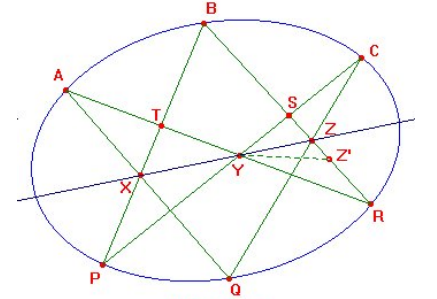
\includegraphics[scale = 0.6]{5.7_1}
\centering
\end{figure}

\section{Clasificación proyectiva de las cuádricas}

En esta sección se tratará de dar, salvo \textit{equivalencia proyectiva}, la lista de todas las cuádricas en el plano proyectivo real y el espacio proyectivo real.

\begin{definition}
Dos cuádricas en espacios proyectivos de la misma dimensión se dirán \ul{proyectivamente equivalentes} si existe alguna proyectividad que transforme una en la otra.
\end{definition}

\begin{theorem}
\label{teo5.7.}
Si dos cuádricas $\mathcal{Q}(q), \mathcal{Q}(q')$ en espacios proyectivos $\mathcal{P}(V), \mathcal
P(V')$ de la misma dimensión sobre el cuerpo $\mathbb{K}$ son proyectivamente equivalentes, entonces $\textup{rg}(q) = \textup{rg}(q')$ y $\textup{Witt}(q) = \textup{Witt}(q')$. Si además $\mathbb{K} = \R$ ó $\mathbb{K} = \mathbb{C}$, entonces el recíproco es cierto.
\end{theorem}

\begin{proof}
Sea $\sigma \colon \mathcal{P}(V) \to \mathcal{P}(V')$ una proyectividad que transforma $\mathcal{Q}(q)$ en $\mathcal{Q}(q')$. Al demostrar el \hyperref[teo5.1.]{\color{blue}Teorema 5.1} se veía que una proyectividad $\sigma = \mathcal{P}(f)$ entre espacios proyectivos transformaba una cuádrica $\mathcal{Q}(q)$ en otra cuádrica $\mathcal{Q}(\Tilde{q})$, con $\tilde{q} = q \circ f^{-1}$, así que se puede suponer que $\tilde{q} = q'$.

\vspace{2mm}
Para la igualdad de rangos, veamos que $\sigma(\mathcal{P}(\textup{Rad}(V))) = \mathcal{P}(\textup{Rad}(V'))$, es decir, que el vértice de $\mathcal{Q}(q')$ es la imagen por $\sigma$ del vértice de $\mathcal{Q}(q)$.
\begin{itemize}
    \item[{\fbox[rb]{$\subset$}}] Sea $u \in \textup{Rad}(V)$. Hay que probar que $\sigma(<u>) = \ <f(u)> \ \in \mathcal{P}(\textup{Rad}(V'))$, es decir, que $f(u) \in \textup{Rad}(V')$. Si $v' \in V'$, por ser $f$ sobreyectiva existe $u' \in V$ tal que $f(u') = v'$, luego
    \[q'(f(u),v') = q'(f(u),f(u')) = q \circ f^{-1}(f(u),f(u')) = q(u,u') = 0\]
    Para la última igualdad se recuerda que $u \in \textup{Rad}(V)$. Esto prueba que $f(u) \in \textup{Rad}(V')$.
    \item[{\fbox[rb]{$\supset$}}] No hay más que utilizar un razonamiento análogo al de la contención anterior sin más que cambiar $f$ por $f^{-1}$ y $q'$ por $q$ donde corresponda.
\end{itemize}

Como $f$ es isomorfismo, se tiene que $\textup{dim}(\textup{Rad}(V)) = \textup{dim}(\textup{Rad}(V'))$, y de $(iv)$ del \hyperref[teo4.1.]{\color{blue}Teorema 4.1} se concluye que $\textup{rg}(q) = \textup{rg}(q')$.

\vspace{2mm}
El índice de Witt coincide con la dimensión de los subespacios isotrópicos maximales de un complemento del radical. Ahora bien, si $P_1 = \ <u_1,v_1>, \mathellipsis, P_l = \ <u_l,v_l>$ son los planos hiperbólicos de la desmposición de Witt, entonces un subespacio isotrópico maximal para $q$ sería $W = \ <u_1,\mathellipsis,u_l>$. Pero como $q = q' \circ f$, entonces $f(W) = \ <f(u_1),\mathellipsis,f(u_l)>$ es un subespacio isotrópico maximal para $q'$. Como ambos tienen la misma dimensión, entonces $\textup{Witt}(q) = \textup{Witt}(q')$ y el teorema se da por demostrado (lo del recíproco no va a probarse).
\end{proof}

\begin{definition}
Una cuádrica no degenerada se dice que es \ul{reglada} si por cada punto de la cuádrica pasan rectas contenidas en la misma.
\end{definition}

Llega el momento de exponer la retahíla de cuádricas proyectivas en el plano proyectivo real $\mathcal{P}_2(\R)$ y el espacio proyectivo real tridimensional $\mathcal{P}_3(\R)$. Para ello, se hará una distinción del rango de $q$ y el índice de Witt, y a partir de ahí podrá deducirse cómo diagonaliza la matriz de $q$ respecto a una cierta base, proporcionando así la ecuación reducida de la cuádrica.

\vspace{2mm}
Por último, se recuerda que el índice de Witt en $\mathbb{C}$ toma siempre su valor máximo, así que para clasificar las cuádricas de $\mathcal{P}_2(\mathbb{C})$ y $\mathcal{P}_3(\mathbb{C})$ no hay más que irse al caso real y quedarse con los casos en los que el índice es máximo, facilitando de sobremanera el asunto. Sin más dilación...

\pagebreak

\thispagestyle{empty}

\vspace*{12mm}

\begin{center} \textbf{Clasificación de las cuádricas de $\mathcal{P}_2(\R)$}

\vspace{6mm}

\footnotesize

\begin{tabular}{|c|c|c|c|m{4cm}|m{4cm}|}
    \hline
     \textbf{rg} & \textbf{Witt} & \textbf{ec. reducida} & \textbf{matriz} & \centering \textbf{descripción} & \centering \textbf{nombre} \tabularnewline
     \hline
     3 & 0 & $ \ \; \: x_0^2+x_1^2+x_2^2 = 0$ & diag\{1,1,1\} & \scriptsize el vacío & \textit{elipse imaginaria} \\
     \hline
     3 & 1 & $-x_0^2+x_1^2+x_2^2 = 0$ & diag\{-1,1,1\} & \scriptsize infinitos puntos & \textit{elipse real} \\
     \hline
     2 & 0 & $\qquad \ \ \, \, x_1^2+x_2^2 = 0$ & diag\{0,1,1\} & \scriptsize la cónica se reduce al vértice, que es un punto & \textit{par de rectas imaginarias que se cortan en un punto real} \\
     \hline
     2 & 1 & $\qquad \: \: \: \: x_1^2-x_2^2 = 0$ & diag\{0,1,-1\} & \scriptsize la directriz tiene dos puntos y el vértice, uno & \textit{par de rectas secantes} \\
     \hline
     1 & 0 & $\qquad \qquad \ \ \; \, x_2^2 = 0$ & diag\{0,0,1\} & \scriptsize la directriz es vacía y el vértice, coincidente con la cónica, una recta & \textit{recta doble} \\
     \hline
     0 & 0 & $\qquad \qquad \quad \: \, \, 0 = 0$ & diag\{0,0,0\} & \scriptsize el total & \\
     \hline
\end{tabular}

\normalsize

\vspace{24mm}

\textbf{Clasificación de las cuádricas de $\mathcal{P}_3(\R)$}

\vspace{6mm}

\footnotesize

\begin{tabular}{|c|c|c|c|m{2.75cm}|m{4cm}|}
    \hline
     \textbf{rg} & \textbf{Witt} & \textbf{ec. reducida} & \textbf{matriz} & \centering \textbf{descripción} & \centering \textbf{nombre} \tabularnewline
     \hline
     4 & 0 & $\ \ \, x_0^2+x_1^2+x_2^2+x_3^2=0$ & diag\{1,1,1,1\} & \scriptsize el vacío & \textit{elipsoide imaginario} \\
     \hline
     4 & 1 & $-x_0^2+x_1^2+x_2^2+x_3^2=0$ & diag\{-1,1,1,1\} & \scriptsize infinitos puntos; no reglada & \textit{elipsoide real no reglado} \\
     \hline
     4 & 2 & $-x_0^2+x_1^2-x_2^2+x_3^2=0$ & diag\{-1,1,-1,1\} & \scriptsize infinitos puntos; por cada uno pasan dos rectas de la cuádrica & \textit{elipsoide real reglado} \\
     \hline
     3 & 0 & $\qquad \quad x_1^2+x_2^2+x_3^2=0$ & diag\{0,1,1,1\} & \scriptsize la cuádrica se reduce al vértice, que es un punto & \textit{cono imaginario de vértice real} \\
     \hline
     3 & 1 & $\qquad \: -x_1^2+x_2^2+x_3^2=0$ & diag\{0,-1,1,1\} & \scriptsize el vértice es un punto; la directriz, una elipse real & \textit{cono real} \\
     \hline
     2 & 0 & $\qquad \qquad \quad \, x_2^2+x_3^2=0$ & diag\{0,0,1,1\} & \scriptsize la cuádrica se reduce al vértice, que es una recta & \textit{par de planos imaginarios secantes en una recta real} \\
     \hline
     2 & 1 & $\qquad \qquad \quad \, x_2^2-x_3^2=0$ & diag\{0,0,1,-1\} & \scriptsize la directriz tiene dos puntos; el vértice es una recta & \textit{par de planos secantes en una recta} \\
     \hline
     1 & 0 & $\qquad \qquad \qquad \quad \ x_3^2=0$ & diag\{0,0,0,1\} & \scriptsize la cuádrica se reduce al vértice, que es un plano & \textit{plano doble} \\
     \hline
     0 & 0 & $\qquad \qquad \qquad \quad \ \ \, 0=0$ & diag\{0,0,0,0\} & \scriptsize el total & \\
     \hline
\end{tabular}

\pagebreak

\normalsize

\end{center}
\begin{example}
Se pide clasificar la cónica real de ecuación
\[\lambda x_0^2 +\lambda x_1^2 + x_2^2 - 2x_0x_1-2x_0x_2+2\lambda x_1 x_2 = 0\]
en función del parámetro $\lambda \in \R$. Respecto de la base canónica, la matriz de la cónica es
\[A = \begin{pmatrix*}[r]
    \lambda & -1 & -1 \\
    -1 & \lambda & \lambda \\
    -1 & \lambda & 1
\end{pmatrix*}\]
Como $\textup{det}(A) = -(\lambda - 1)(\lambda^2-1)$, la cónica degenera cuando $\lambda = 1$ y cuando $\lambda = -1$. Primero se estudiará el caso $\lambda \notin \{-1,1\}$. Para determinar el índice de Witt, habrá que encontrar una base ortogonal de $\R^3$. Se empieza por tomar un vector no isótropo, por ejemplo $u_0 = (0,0,1)$, que verifica
\[q(u_0) = \begin{pmatrix}
    0 & 0 & 1
\end{pmatrix} \begin{pmatrix*}[r]
    \lambda & -1 & -1 \\
    -1 & \lambda & \lambda \\
    -1 & \lambda & 1
\end{pmatrix*} \begin{pmatrix}
    0 \\
    0 \\
    1
\end{pmatrix} = 1 \neq 0
\]
Ahora se calcula el complemento ortogonal de $<u>$. Dado $x = (x_0,x_1,x_2) \in \R^3$, se tiene
\[q(u_0,x) = 0 \iff \begin{pmatrix}
    0 & 0 & 1
\end{pmatrix} \begin{pmatrix*}[r]
    \lambda & -1 & -1 \\
    -1 & \lambda & \lambda \\
    -1 & \lambda & 1
\end{pmatrix*} \begin{pmatrix}
    x_0 \\
    x_1 \\
    x_2
\end{pmatrix} = 0 \iff -x_0+\lambda x_1+x_2 = 0\]
Se continúa eligiendo un vector que satisfaga esta ecuación y sea no isótropo. Uno de ellos es $u_1=(1,0,1)$, que satisface
\[q(u_1) = \begin{pmatrix}
    1 & 0 & 1
\end{pmatrix} \begin{pmatrix*}[r]
    \lambda & -1 & -1 \\
    -1 & \lambda & \lambda \\
    -1 & \lambda & 1
\end{pmatrix*} \begin{pmatrix}
    1 \\
    0 \\
    1
\end{pmatrix} = \lambda - 1 \neq 0\]
Recuérdese que se está estudiando el caso $\lambda \notin \{-1,1\}$. Se calcula el complemento ortogonal de $u_1$: dado $x = (x_0,x_1,x_2) \in \R^3$, se tiene
\[q(u_1,x) = 0 \iff \begin{pmatrix}
    1 & 0 & 1
\end{pmatrix} \begin{pmatrix*}[r]
    \lambda & -1 & -1 \\
    -1 & \lambda & \lambda \\
    -1 & \lambda & 1
\end{pmatrix*} \begin{pmatrix}
    x_0 \\
    x_1 \\
    x_2
\end{pmatrix} = 0 \iff (\lambda-1)x_0+(\lambda-1)x_1 = 0\]
El vector isótropo que se busca ahora tendrá que verificar
\[
\spalignsys{
 -x_0 + \lambda x_1 + x_2 = 0 ;
 x_0 + x_1 \. \. = 0
}
\]
Cae del cielo el vector $u_2 = (1,-1,1+\lambda)$, que cumple
\[q(u_2) = \begin{pmatrix}
    1 &-1 & 1+\lambda
\end{pmatrix} \begin{pmatrix*}[r]
    \lambda & -1 & -1 \\
    -1 & \lambda & \lambda \\
    -1 & \lambda & 1
\end{pmatrix*} \begin{pmatrix*}[c]
    \ \; \, 1 \\
    -1 \\
    1+\lambda
\end{pmatrix*} = 1-\lambda^2 \neq 0\]
Acabado el proceso de diagonalización, la matriz de $q$ respecto de la base $\{u_0,u_1,u_2\}$ es
\[\begin{pmatrix}
    1 & 0 & 0 \\
    0 & \lambda -1 & 0 \\
    0 & 0 & 1-\lambda^2
\end{pmatrix}\]
Se distinguen varios casos:
\begin{itemize}
    \item[(i)] Si $\lambda < -1$, respecto de la base $\{u_0,\frac{1}{\sqrt{1-\lambda}} \, u_1, \frac{1}{\sqrt{\lambda^2-1}} \, u_2 \}$ la matriz de $q$ queda
    \[\begin{pmatrix}
    1 & 0 & 0 \\
    0 & -1 & 0 \\
    0 & 0 & -1
    \end{pmatrix}\]
    \item[(ii)] Si $-1 < \lambda < 1$, respecto de la base $\{u_0,\frac{1}{\sqrt{1-\lambda}} \, u_1, \frac{1}{\sqrt{1-\lambda^2}} \, u_2 \}$ la matriz de $q$ queda
    \[\begin{pmatrix}
    1 & 0 & 0 \\
    0 & -1 & 0 \\
    0 & 0 & 1
    \end{pmatrix}\]
    \item[(iii)] Si $1 < \lambda$, respecto de la base $\{u_0,\frac{1}{\sqrt{\lambda-1}} \, u_1, \frac{1}{\sqrt{\lambda^2-1}} \, u_2 \}$ la matriz de $q$ queda
    \[\begin{pmatrix}
    1 & 0 & 0 \\
    0 & 1 & 0 \\
    0 & 0 & -1
    \end{pmatrix}\]
\end{itemize}
En todos los casos se manifiesta un plano hiperbólico, de forma que el índice de Witt es 1 y estamos ante una \textit{elipse real}.

\vspace{2mm}
\noindent
Si fuese $\lambda = 1$, la matriz
\[A = \begin{pmatrix*}[r]
    1 & -1 & -1 \\
    -1 & 1 & 1 \\
    -1 & 1 & 1
\end{pmatrix*}\]
es de rango 1 y la cónica es una \textit{recta doble}. Por hacer algo más, se tratará de encontrar una base respecto de la cual la ecuación reducida de la recta sea $x_2^2 = 0$. Utilizando los vectores anteriores, se observa que respecto de la base $\{u_1,u_2,u_0\}$ la matriz de $q$ es
\[\begin{pmatrix*}
    0 & 0 & 0 \\
    0 & 0 & 0 \\
    0 & 0 & 1
\end{pmatrix*}\]
y la ecuación reducida, $x_2^2 = 0$. Se observa también que el vértice es $\mathcal{P}(<u_1>,<u_2>)$.

\vspace{2mm}
\noindent
Solo falta por examinar el caso $\lambda = -1$. La matriz
\[A = \begin{pmatrix*}[r]
    -1 & -1 & -1 \\
    -1 & -1 & -1 \\
    -1 & -1 & 1
\end{pmatrix*}\]
es de rango 2. El vértice consta de un punto, y aprovechando de nuevo los vectores conocidos se observa que dicho punto es $P = \ <v_0> \ = \ <(1,-1,0)>$. Un suplemento del radical es, por ejemplo,
\[W = \ <(0,1,0),(0,0,1)>\]
El vector $v_1 = (0,0,1) \in W$ cumple
\[q(v_1) = \begin{pmatrix}
    0 & 0 & 1
\end{pmatrix} \begin{pmatrix*}[r]
    -1 & -1 & -1 \\
    -1 & -1 & -1 \\
    -1 & -1 & 1
\end{pmatrix*} \begin{pmatrix}
    0 \\
    0 \\
    1
\end{pmatrix} = 1 \neq 0\]
Ahora habrá que encontrar uno ortogonal a $v_1$, distinto de $v_0$ y no isótropo. Para ello, si $x = (x_0,x_1,x_2) \in \R^3$, entonces
\[q(v_1,x) = 0 \iff \begin{pmatrix}
    0 & 0 & 1
\end{pmatrix} \begin{pmatrix*}[r]
    -1 & -1 & -1 \\
    -1 & -1 & -1 \\
    -1 & -1 & 1
\end{pmatrix*} \begin{pmatrix}
    x_0 \\
    x_1 \\
    x_2
\end{pmatrix} = 0 \iff -x_0-x_1+x_2=0\]
Por ejemplo, $v_2 = (0,1,1)$ sirve, pues se tiene
\[q(v_2) = \begin{pmatrix}
    0 & 1 & 1
\end{pmatrix} \begin{pmatrix*}[r]
    -1 & -1 & -1 \\
    -1 & -1 & -1 \\
    -1 & -1 & 1
\end{pmatrix*} \begin{pmatrix}
    0 \\
    1 \\
    1
\end{pmatrix} = -2 \neq 0\]
En la base $\{v_0,v_1,\frac{1}{\sqrt{2}} v_2\}$, la matriz de $q$ es
\[\begin{pmatrix*}[r]
    0 & 0 & 0 \\
    0 & 1 & 0 \\
    0 & 0 & -1
\end{pmatrix*}\]
así que se concluye que la cónica es el \textit{par de rectas secantes} $x_1^2-x_2^2=0$.
\end{example}

\chapter{Cuádricas en el espacio afín}

\section{Introducción}

Las cuádricas proyectivas se definieron de forma que al restringirse al afín, se obtengan las cuádricas afines de la \hyperref[def5.1.]{\color{blue}Definición 5.1}. Sin embargo, siguiendo la tónica general de esta asignatura de estudiar el afín como aquello que resulta de eliminar un hiperplano del espacio proyectivo, la definición oficial de \textit{cuádrica afín} será la siguiente:

\begin{definition}
Dada una cuádrica $\mathcal{Q}(q)$ en un espacio proyectivo $\mathcal{P}(V)$ y un hiperplano $\mathcal{P}(H)$, el conjunto
\[\mathcal{Q}(q, H) \equiv \mathcal{Q}(q) \setminus \mathcal{P}(H) = \mathcal{Q}(q) \cap \mathcal{A}(V,H)\]
se denomina \ul{cuádrica afín}.
\end{definition}

Como indica la notación, una cuádrica afín no solo depende de la forma cuadrática $q$, sino también del hiperplano $\mathcal{P}(H)$. Una cuádrica proyectiva puede dar lugar a distintas cuádricas afines dependiendo del hiperplano del infinito que se escoja.

\begin{example}
En $\mathcal{P}_2(\R)$, se considera la cónica $\mathcal{Q}(q) \equiv x_1^2 =0$. Si se toma como recta del infinito la de ecuación $x_0 = 0$, entonces $\mathcal{Q}(q,H)$ consta de los puntos cuyas coordenadas homogéneas $(x_0,x_1,x_2)$ verifican $x_0 \neq 0$ y $x_1 = 0$. En cartesianas, serían los puntos de coordenadas $(x,y)$ con $x = 0$.

\vspace{2mm}
\noindent
Ahora bien, tomando como recta del infinito aquella de ecuación $x_1 = 0$, entonces $\mathcal{Q}(q,H)$ consta de los puntos cuyas coordenadas homogéneas $(x_0,x_1,x_2)$ verifican $x_1 = 0$ y $x_1 \neq 0$. Semejante absurdo dice que la cónica afín es el vacío.
\end{example}

\begin{definition}
Dada una cuádrica proyectiva $\mathcal{Q}(q)$ y un hiperplano $\mathcal{P}(H)$, se le llama \ul{cuádrica en el infinito de la cuádrica afín $\mathcal{Q}(q,H)$} a $\mathcal{Q}(q_H) = \mathcal{Q}(q) \cap \mathcal{P}(H)$.
\end{definition}
\begin{proposition}
Dada una cuádrica $\mathcal{Q}(q)$ y un hiperlano $\mathcal{P}(H)$ de un espacio proyectivo, se tiene
\[\mathcal{Q}(q) = \mathcal{Q}(q,H) \cup \mathcal{Q}(q_H)\]
\end{proposition}

\begin{proof}
    Inmediata.
\end{proof}

Estaría bien que la definición que se ha dado de cuádrica afín no difiriese de aquella que se vio al inicio del tema anterior. En efecto,
\begin{proposition}
Dado un conjunto de puntos $\mathcal{C}$ de un espacio afín $\mathbb{K}^n$ descrito por una ecuación del tipo
\[p(y_1,\mathellipsis,y_n) = 0\]
con $p$ un polinomio de segundo grado sobre $\mathbb{K}$, existe al menos una cuádrica proyectiva $\mathcal{Q}(q)$ en $\mathcal{P}_n(\mathbb{K})$ tal que $\mathcal{Q}(q,H) = \mathcal{C}$.
\end{proposition}

\begin{proof}
Tomando como hiperplano del infinito el de ecuación cartesiana $x_0 = 0$, la cuádrica $\mathcal{Q}(q)$ buscada no es más que la que define la forma cuadrática
\[q(x_0,\mathellipsis,x_n) = x_0^2\, p\biggl(\frac{x_1}{x_0},\mathellipsis,\frac{x_n}{x_0} \biggr)\]
como se comprueba inmediatamente.
\end{proof}

\begin{theorem}
    Si $f \colon V \to V'$ es un isomorfismo lineal entre espacios vectoriales, entonces cada cuádrica afín $\mathcal{Q}(q,H)$ en $\mathcal{A}(V,H)$ se transforma por la afinidad $\mathcal{A}(f)$ en una cuádrica afín de $\mathcal{A}(V',f(H))$.
\end{theorem}

\begin{proof}
En virtud del \hyperref[teo5.1.]{\color{blue}Teorema 5.1}, su demostración y la definición de cuádrica afín, es inmediato comprobar que la afinidad $\mathcal{A}(f)$, que no es más que la restricción de una proyectividad, envía $\mathcal{Q}(q,H)$ en la cuádrica $\mathcal{Q}(q \circ f^{-1}, f(H))$.
\end{proof}

\section{Posición relativa de una cuádrica y un hiperplano}

\begin{theorem}
\label{teo6.2.}
Sea $H$ un hiperplano de un espacio vectorial $V$ de dimensión $n \geq 2$ sobre $\mathbb{K}$ en el que hay definida una forma cuadrática $q$.

\begin{itemize}
    \item[(i)] Si $H^\perp \not\subset H$, entonces para cada $u \in H^\perp \setminus H$ puede escribirse
    \[V = \ <u> \oplus \ H\]
    siendo la suma ortogonal-directa.
    \item[(ii)] Si $H^\perp \subset H$, existen un subespacio $U$ y un par hiperbólico $(u,v)$ con $v \in H^\perp \setminus \textup{Rad}(V)$ y $u \notin H$ de forma que
    \[V = \ <u,v> \oplus \ U \qquad H = \ <v> \oplus \ U\]
    siendo cada suma ortogonal-directa.
\end{itemize}

\end{theorem}

\begin{proof}
Para probar $(i)$, tómese $u \in H^\perp \setminus H$. Entonces $<u> \cap \ H = 0$ y por la fórmula de Grassmann se tiene $V = \ <u> \oplus \ H$. La ortogonalidad de la suma es evidente.

\vspace{2mm}
En cuanto al apartado $(ii)$, supóngase que $H^\perp \subset H$. Echando mano de la \hyperref[prop4.1.]{\color{blue}Proposición 4.2}, se verifica
\[\textup{dim}(H^\perp) = \textup{dim}(V) - \textup{dim}(H) + \textup{dim}(H \cap \textup{Rad}(V)) = 1 + \textup{dim}(H \cap \textup{Rad}(H))\]
y como $H \subset V$, entonces $V^\perp = \textup{Rad}(V) \subset H^\perp \subset H$, luego $H \cap \textup{Rad}(V) = \textup{Rad}(V)$ y por tanto $\textup{Rad}(V)$ es un hiperplano de $H^\perp$. Se puede tomar entonces $v \in H^\perp \setminus \textup{Rad}(V)$. Se tiene que $v$ es isótropo (pues $v \in H^\perp$ y $v \in H$) y además, siguiendo la demostración de la \hyperref[prop4.4.]{\color{blue}Proposición 4.4}, existe $u \in V$ tal que $(u,v)$ es un par hiperbólico. Como $q(u,v) = 1 \neq 0$, se sigue que $u \notin H$. El subespacio $U$ tal que
\[V = \ <u,v> \oplus \ U\]
es proporcionado por el teorema del sumando directo. Por último, como $<v> \ \subset H^\perp$ implica $H \subset (H^\perp)^\perp \subset \ <v>^\perp$ y además
\[\textup{dim}(<v>^\perp) = \textup{dim}(V) - \textup{dim}(<v>) + \textup{dim}(<v> \cap \ \textup{Rad}(V)) = \textup{dim}(V) -1\]
entonces $H = \ <v>^\perp$. El hecho de que $U \subset \ <v>^\perp \ = H$ (esto se debe a $<v> \ \subset U^\perp$) y que $\textup{dim}(U) = \textup{dim}(V) - 2$ permite escribir $H = \ <v> \oplus \ U$ ortogonal-directamente.
\end{proof}

\begin{definition}
Una cuádrica afín $\mathcal{Q}(q,H)$ para la que se tenga $H^\perp \not\subset H$ será denominada \ul{cuádrica con centro}. En el caso $H^\perp \subset H$, se hablará de \ul{paraboloides}.
\end{definition}

\begin{proposition}
\label{prop6.3.}
    Los paraboloides proceden de cuádricas proyectivas tangentes al hiperplano impropio.
\end{proposition}

\begin{proof}
Dado un paraboloide $\mathcal{Q}(q,H)$, que se tenga $0 \neq H^\perp \cap H = \textup{Rad}(H)$ significa que la restricción $q_H$ degenera, o sea, $\mathcal{P}(H)$ es tangente a la cuádrica proyectiva $\mathcal{Q}(q)$.
\end{proof}

A continuación, se va a justificar a qué viene la denominación de \say{cuádrica con centro} para las cuádricas afines en las condiciones del primer apartado del teorema anterior.

\vspace{2mm}
Sea $\mathcal{Q}(q,H)$ una cuádrica con centro en un espacio afín $\mathcal{A}(V,H)$. Si se toma una base ortogonal $\{u_1,\mathellipsis,u_n\}$ de $H$ y se escoge $u \in H^\perp \setminus H$, por el primer apartado del teorema anterior, la base $\{u,u_1,\mathellipsis,u_n\}$ de $V$ es ortogonal, y respecto de ella, la ecuación de la cuádrica proyectiva sería
\[\lambda_0 x_0^2+\lambda_1 x_1^2+\mathellipsis+\lambda_n x_n^2 = 0\]
Al pasar a coordenadas cartesianas se obtiene la ecuación de la cuádrica afín $\mathcal{Q}(q,H)$:
\[\lambda_0+\lambda_1 y_1^2+\mathellipsis+\lambda_n y_n^2 = 0 \tag{1}\]
La matriz de $q$ en la base $\{u,u_1,\mathellipsis,u_n\}$ sería
\[\left( \begin{array}{c|ccc}
    \lambda_0 & 0 & \mathellipsis & 0 \\ \hline
    0 & \lambda_1 & \mathellipsis & 0 \\
    \vdots & \vdots & \ddots & \vdots \\
    0 & 0 & \mathellipsis & \lambda_n
\end{array} \right)\]
Como $u \notin H$, entonces $O = \ <u> \ \in \mathcal{A}(V,H)$. Respecto de la base anterior, sus coordenadas  homogéneas son $(1,0,\mathellipsis,0)$, así que al pasar a cartesianas quedaría una $n$-upla de ceros. 

\vspace{2mm} Además, de la ecuación de la cuádrica afín se deduce que si el punto $P$ de coordenadas $(\alpha_1,\mathellipsis,\alpha_n)$ está en la cuádrica, entonces el punto $-P$ de coordenadas $(-\alpha_1,\mathellipsis,-\alpha_n)$ también. Ahora bien, $-P$ no es más que el simétrico de $P$ respecto de $u$, que en la base ya mencionada es el origen de coordenadas. Se deduce que $O$ hace de centro de simetría, lo que justifica que las cuádricas con centro se llamen como tal.

\vspace{2mm}
Por otro lado, sea $\mathcal{Q}(q,H)$ un paraboloide en el afín $\mathcal{A}(V,H)$ y considérese la base $\{u,v,u_2,\mathellipsis,u_n\}$, donde $(u,v)$ es el par hiperbólico ofrecido por el apartado segundo del teorema anterior y $\{u_2,\mathellipsis,u_n\}$ es una base ortogonal del subespacio $U$. Respecto de esta base, la matriz de $\mathcal{Q}(q)$ es
\[\left( \begin{array}{c|cccc}
    0 & 1 & 0 & \mathellipsis & 0 \\ \hline
    1 & 0 & 0 & \mathellipsis & 0 \\
    0 & 0 & \lambda_2 & \mathellipsis & 0 \\
    \vdots & \vdots & \vdots & \ddots & \vdots \\
    0 & 0 & 0 & \mathellipsis & \lambda_n
\end{array} \right)\]
y la ecuación de $\mathcal{Q}(q)$,
\[2x_0x_1+\lambda_2 x_2^2 + \mathellipsis+\lambda_nx_n^2 = 0\]
y la de $\mathcal{Q}(q,H)$, pasando a cartesianas,
\[2y_1+\lambda_2 y_2^2 + \mathellipsis+\lambda_ny_n^2 = 0 \tag{2}\]
Ahora no hay centro de simetría, pero sí eje, y es precisamente la recta
\[r \equiv \begin{cases}
    y_2 = 0 \\
    y_3 = 0 \\
    \ \vdots \\
    y_n = 0
\end{cases}\]
En efecto, si $P = (\alpha_1, \alpha_2,\mathellipsis,\alpha_n) \in \mathcal{Q}(q,H)$, entonces $P' = (\alpha_1, -\alpha_2,\mathellipsis,-\alpha_n) \in \mathcal{Q}(q,H)$, y este último punto no es más que el simétrico de $P$ con respecto de $r$.

\begin{definition}
La expresión $(1)$ o $(2)$ se denomina \ul{ecuación reducida} de la cuádrica afín, según sea un paraboloide o una cuádrica con centro.
\end{definition}

\begin{definition}
Si $\{u,u_1,\mathellipsis,u_n\}$ es la base en la que se expresa la ecuación reducida de una cuádrica $\mathcal{Q}(q,H)$ en el afín $\mathcal{A}(V,H)$, se llamará \ul{eje de la cuádrica} a la parte afín de cada recta $\overline{P_0P_i}$, donde $P_0 = \ <u>$ y $P_i = \ <u_i>$ para todo $i \in \{1,2,\mathellipsis,n\}$.
\end{definition}

\begin{definition}
A las intersecciones de una cuádrica afín con sus ejes se les llama \ul{vértices}.
\end{definition}

A falta de palabras en el diccionario de la lengua española, la que se ha escogido en esta definición puede causar confusión con aquella de la \hyperref[def5.4.]{\color{blue}Definición 5.4}. 

\vspace{2mm}
Obsérvese que un paraboloide siempre tiene al menos un vértice (concretamente, el punto $O = \ <u>$), y si no degenera (lo que signficaría $0 \notin \{\lambda_2,\mathellipsis,\lambda_n\}$) entonces se comprueba que el vértice consta de un único punto. Ahora bien, una cuádrica con centro no tendría por qué tener vértice...

\begin{example}
Sea $\mathcal{Q}(q,H)$ una cuádrica afín con centro que no pasa por el origen, es decir, con $\lambda_0 \neq 0$, donde
\[\lambda_0 x_0^2 + \lambda_1 x_1^2 + \mathellipsis + \lambda_nx_n^2 = 0\]
es su ecuación reducida. La intersección de la cuádrica con el eje $\overline{P_0P_1}$ debe cumplir
\[\lambda_0+\lambda_1\alpha^2 = 0\]
donde $(\alpha,0,\mathellipsis,0)$ son las coordenadas de un punto cualquiera de dicho eje. Ahora bien, la ecuación anterior no tiene soluciones en caso de que $\lambda_1 = 0$ o que $-\frac{\lambda_1}{\lambda_0}$ no tenga raíz cuadrada.
\end{example}

\begin{definition}
Se define el \ul{centro} de una cuádrica con centro $\mathcal{Q}(q,H)$ como la parte afín del subespacio $\mathcal{P}(H)^\perp$.
\end{definition}

\begin{proposition}
El centro de una cuádrica con centro no degenerada se reduce al polo del hiperplano del infinito.
\end{proposition}

\begin{proof}
Consecuencia directa de que los $\lambda_i$ de la ecuación reducida son todos no nulos, y por tanto la cuádrica proyectiva de la que procede la afín no degenera.
\end{proof}

\begin{definition}
Una cuádrica $\mathcal{Q}(q,H)$ no degenerada y con centro será un \ul{elipsoide} si la cuádrica en el infinito es vacía. En caso contrario, se hablará de \ul{hiperboloides}.
\end{definition}

Nótese que una cuádrica con centro no degenerada no puede ser tangente al infinito, como probaría un argumento similar al de la \hyperref[prop6.3.]{\color{blue}Proposición 6.3}.

\begin{definition}
En dimensión 2, a los elipsoides se les llama \ul{elipses}; a los hiperboloides, \ul{hipérbolas}; y a los paraboloides no degenerados, \ul{parábolas}.
\end{definition}

\begin{definition}
Dada una cuádrica afín no degenerada con centro, se definen los \ul{diámetros} como la parte afín de los hiperplanos polares de los puntos del infinito.
\end{definition}

\begin{definition}
Por \ul{asíntota} se entiende a una recta tangente a una cuádrica en un punto del infinito.
\end{definition}

\begin{figure}[h]
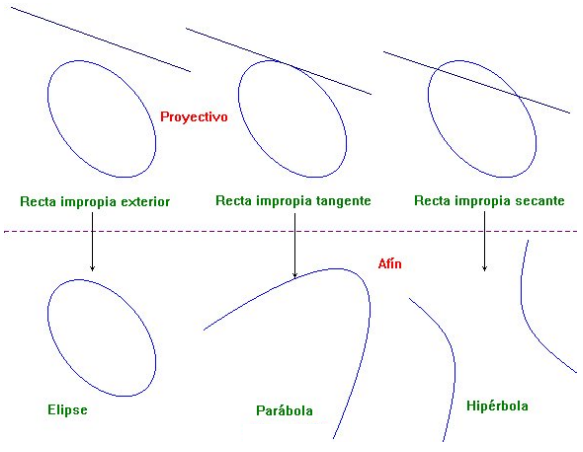
\includegraphics[scale = 0.5]{6.3_1}
\centering
\end{figure}

\begin{example}
Se considera la cónica real de ecuación
\[1-2y+2x^2-y^2=0\]
cuya extensión proyectiva tiene ecuación
\[x_0^2-2x_0x_2+2x_1^2-x_2^2=0\]
respecto a la base canónica de $\R^3$, donde el hiperplano del infinito $H$ que se ha tomado es el de ecuación $x_0 = 0$. La matriz sería entonces
\[A = \begin{pmatrix*}[r]
    1 & 0 & -1 \\
    0 & 2 & 0 \\
    -1 & 0 & -1
\end{pmatrix*}\]
Habrá que calcular $H^\perp$ para ver si se trata de una cónica con centro o de un paraboloide. Se tiene que $H^\perp = \ <(0,1,0),(0,0,1)>^\perp$, así que habrá que imponer las condiciones
\begin{itemize}
    \item $\displaystyle \begin{pmatrix}
        0 & 1 & 0 
    \end{pmatrix}
    \begin{pmatrix*}[r]
    1 & 0 & -1 \\
    0 & 2 & 0 \\
    -1 & 0 & -1
    \end{pmatrix*} \begin{pmatrix}
        x_0 \\
        x_1 \\
        x_2
    \end{pmatrix} = 0 \iff 2x_1 = 0$
   \item $\displaystyle \begin{pmatrix}
        0 & 0 & 1 
    \end{pmatrix}
    \begin{pmatrix*}[r]
    1 & 0 & -1 \\
    0 & 2 & 0 \\
    -1 & 0 & -1
    \end{pmatrix*} \begin{pmatrix}
        x_0 \\
        x_1 \\
        x_2
    \end{pmatrix} = 0 \iff -x_0 -x_2 = 0$
\end{itemize}
Por tanto, $H^\perp = \ <(1,0,-1)>$ y puede deducirse que la cónica tiene centro. Ahora habrá que elegir $u \in H^\perp \setminus H$, por ejemplo $u = (1,0,-1)$, y se tendrá que completar a una base ortogonal, propósito que sirven los vectores $u_1 = (0,1,0)$ y $u_2 = (0,0,1)$. En la base $\{u,u_1,u_2\}$, la matriz de $q$ sería
\[\begin{pmatrix*}[r]
    2 & 0 & 0 \\
    0 & 2 & 0 \\
    0 & 0 & -1
\end{pmatrix*}\]
y la ecuación reducida,
\[2+2x^2-y^2 = 0\]
A continuación se calculará el centro de la cónica, o sea, la parte afín del punto de coordendas homogéneas $(1,0,-1)$. Pasando a coordenadas cartesianas, se obtendría $P = (0,-1)$. Se procede entonces al cálculo de $\overline{P_0P_1}$ y $\overline{P_0P_2}$ para hallar los ejes, donde \[P_0 = \ <(1,0,-1)> \qquad P_1 = \ <(0,1,0)> \qquad P_2 = \ <(0,0,1)>\]
Se tiene que
\begin{itemize}
    \item $\displaystyle \overline{P_0P_1} \equiv \begin{vmatrix}
        x_0 & x_1 & \phantom{-}x_2 \\
        1 & 0 & -1 \\
        0 & 1 & \phantom{-}0
    \end{vmatrix} = 0 \iff \overline{P_0P_1} \equiv \begin{cases}
        x_0+x_2 = 0
    \end{cases}$
    \item $\displaystyle \overline{P_0P_2} \equiv \begin{vmatrix}
        x_0 & x_1 & \phantom{-}x_2 \\
        1 & 0 & -1 \\
        0 & 0 & \phantom{-}1
    \end{vmatrix} = 0 \iff \overline{P_0P_2} \equiv \begin{cases}
        x_1 = 0
    \end{cases}$
\end{itemize}
así que las respectivas partes afines (es decir, los ejes) serían, pasando a coordenadas cartesianas,
\[\overline{P_0P_1} \cap \R^2 \equiv \begin{cases}
    1 + y = 0
\end{cases}\qquad \overline{P_0P_2} \cap \R^2 \equiv \begin{cases}
    x = 0
\end{cases}\]
También habrá que ver si estamos ante una elipse o una hipérbola. Se tendrá que confirmar si la extensión proyectiva $\mathcal{Q}(q)$ corta o no al hiperplano del infinito $\mathcal{P}(H)$. Sustituyendo $x_0$ en la ecuación de $\mathcal{Q}(q)$, se obtiene que
\[\mathcal{Q}(q) \cap \mathcal{P}(H) = \{<(0,1,\sqrt{2})>,<(0,1,-\sqrt{2})>\} = \{R, S\}\]
así que la cónica es una hipérbola. Para terminar de exprimir el ejemplo, se hallarán las asíntotas de la hipérbola. Dado un punto $P$ de la cónica, la recta tangente en dicho punto será $P^\perp$. Como $R$ y $S$ son los puntos de la cónica que están también en el infinito, entonces las asíntotas $r = R^\perp \cap \R^2$ y $s = S^\perp \cap \R^2$ vendrán dadas por

\[ r \equiv \begin{pmatrix}
        0 & 1 & \sqrt{2}
    \end{pmatrix}
    \begin{pmatrix*}[r]
    1 & 0 & -1 \\
    0 & 2 & 0 \\
    -1 & 0 & -1
    \end{pmatrix*} \begin{pmatrix}
        1 \\
        x \\
        y
    \end{pmatrix} = 0  \qquad s \equiv \begin{pmatrix}
        0 & 1 & -\sqrt{2}
    \end{pmatrix}
    \begin{pmatrix*}[r]
    1 & 0 & -1 \\
    0 & 2 & 0 \\
    -1 & 0 & -1
    \end{pmatrix*} \begin{pmatrix}
        1 \\
        x \\
        y
    \end{pmatrix} = 0\]
lo que proporciona las ecuaciones
\[r \equiv \begin{cases}
        -\sqrt{2}+2x-\sqrt{2}y = 0
    \end{cases} \qquad s \equiv \begin{cases}
        \sqrt{2}+2x+\sqrt{2}y = 0
    \end{cases}\]
\end{example}

\begin{figure}[h]
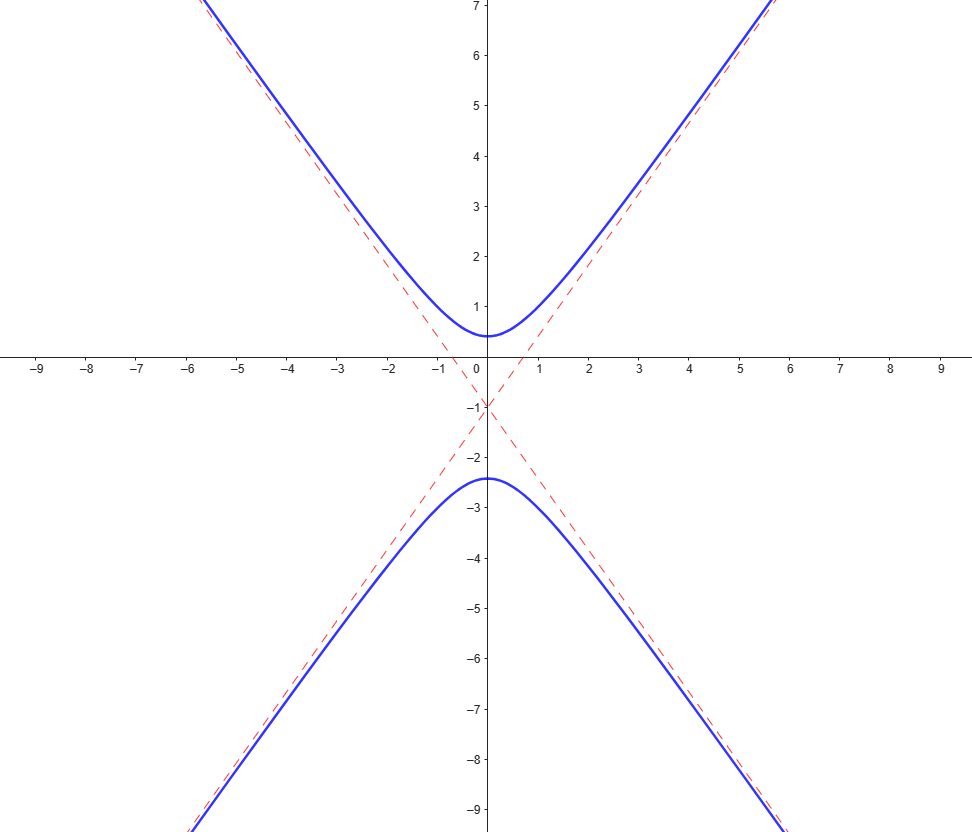
\includegraphics[scale = 0.40]{6.3_2}
\centering
\end{figure}

\begin{example}
Se considera la cónica real de ecuación
\[4x+4y+2x^2-4xy+2y^2=0\]
cuya extensión proyectiva tiene ecuación
\[4x_0x_1+4x_0x_2+2x_1^2-4x_1x_2+2x_2^2=0\]
respecto a la base canónica de $\R^3$, donde el hiperplano del infinito $H$ que se ha tomado es el de ecuación $x_0 = 0$. La matriz sería entonces
\[A = \begin{pmatrix*}[r]
    0 & 2 & 2 \\
    2 & 2 & -2 \\
    2 & -2 & 2
\end{pmatrix*}\]
Habrá que calcular $H^\perp$ para ver si se trata de una cónica con centro o, por contrario, de un paraboloide. Se tiene que $H^\perp = \ <(0,1,0),(0,0,1)>^\perp$, así que habrá que imponer las condiciones
\begin{itemize}
    \item $\displaystyle \begin{pmatrix}
        0 & 1 & 0 
    \end{pmatrix}
\begin{pmatrix*}[r]
    0 & 2 & 2 \\
    2 & 2 & -2 \\
    2 & -2 & 2
\end{pmatrix*} \begin{pmatrix}
        x_0 \\
        x_1 \\
        x_2
    \end{pmatrix} = 0 \iff x_0+x_1-x_2=0$
   \item $\displaystyle \begin{pmatrix}
        0 & 0 & 1 
    \end{pmatrix}
\begin{pmatrix*}[r]
    0 & 2 & 2 \\
    2 & 2 & -2 \\
    2 & -2 & 2
\end{pmatrix*} \begin{pmatrix}
        x_0 \\
        x_1 \\
        x_2
    \end{pmatrix} = 0 \iff x_0-x_1+x_2 = 0$
\end{itemize}
Por tanto, $H^\perp = \ <(0,1,1)>$ y puede deducirse que la cónica es un paraboloide. Es más, después de calcular el determinante de $A$ se puede afirmar la no degeneración y se está entonces ante una parábola. 

\vspace{3mm}
\noindent En búsqueda de una base en condiciones, habrá que elegir $v \in H^\perp \setminus \textup{Rad}(\R^3) = H^\perp$, por ejemplo $v = (0,1,1)$, y se tendrá que encontrar su media naranja que proporcione un par hiperbólico. Sirve el vector $u = (1,0,0)$, isótropo y no ortogonal a $v$, verificando $q(u,v) = 4$. 

\vspace{3mm}
\noindent Para terminar de encontrar la base adecuada, habrá que calcular $U = \ <u,v>^\perp$. Haciendo las cuentas pertinentes se obtiene $U= \ <(0,1,-1)> \ = \ <w>$. En la base $\{\frac{1}{4}u,v,w\}$, la matriz de $q$ sería
\[\begin{pmatrix*}[r]
    0 & 1 & 0 \\
    1 & 0 & 0 \\
    0 & 0 & 8
\end{pmatrix*}\]
y la ecuación reducida,
\[2x+8y^2 = 0\]
El vértice de la parábola es el punto $<u>$ que tiene coordenadas homogéneas $(1/4,0,0)$ y cartesianas $(0,0)$ respecto de la base anterior. Los ejes son las partes afines de las rectas $\overline{P_0P_1}$ y $\overline{P_0P_2}$, donde \[P_0 = \ <(1/4,0,0)> \qquad P_1 = \ <(0,1,1)> \qquad P_2 = \ <(0,1,-1)>\]
Se tiene que
\begin{itemize}
    \item $\displaystyle \overline{P_0P_1} \cap \R^2 \equiv \begin{vmatrix}
        1 & x & y \\[2pt]
         \frac{1}{4} & 0 & 0 \\[2pt]
        0 & 1 & 1
    \end{vmatrix} = 0 \iff \overline{P_0P_1} \equiv \begin{cases}
        x-y = 0
    \end{cases}$
    \item $\displaystyle \overline{P_0P_2} \cap \R^2 \equiv \begin{vmatrix}
        1 & x & \phantom{-}y \\[2pt]
        \frac{1}{4} & 0 & \phantom{-}0 \\[2pt]
        0 & 1 & -1
    \end{vmatrix} = 0 \iff \overline{P_0P_2} \equiv \begin{cases}
        x+y = 0
    \end{cases}$
\end{itemize}

\begin{figure}[h]
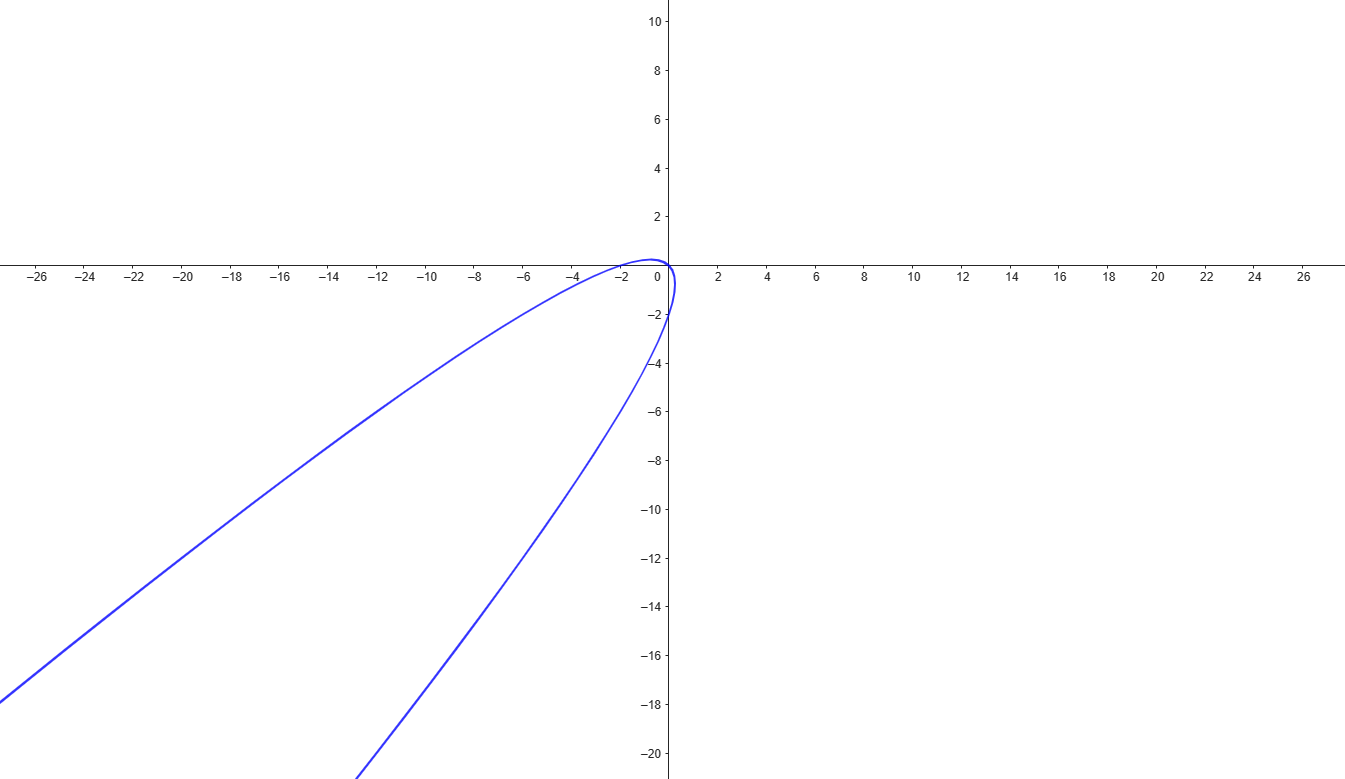
\includegraphics[scale = 0.3]{6.3_3}
\centering
\end{figure}

\end{example}

\section{Clasificación afín de las cuádricas}

En esta sección se tratará de dar la lista de todos los pares $(q,H)$ que definen las cuádricas afines $\mathcal{Q}(q,H)$ de $\R^2$ y $\R^3$, salvo \textit{equivalencia afín}.

\begin{definition}
Sean $V, V'$ dos espacios vectoriales sobre el mismo cuerpo provistos de sendas formas cuadráticas $q, q'$ e hiperplanos $H, H'$. Se dirá que los pares $(q,H)$ y $(q',H')$ son \ul{afínmente equivalentes} si existe un isomorfismo lineal $f \colon V \to V'$ tal que $q = q' \circ f$ y $f(H) = H'$.
\end{definition}

\begin{theorem}
Si $(q,H)$ y $(q',H')$ son afínmente equivalentes, entonces
\setlength{\columnsep}{0cm}
\setlength{\columnseprule}{0pt}
\begin{multicols}{2}
\noindent
\begin{align*}
    \textup{rg}(q) &= \textup{rg}(q') \\
    \textup{rg}(q_H) &= \textup{rg}(q_{H'}')
\end{align*}
\begin{align*}
    \textup{Witt}(V,q) &= \textup{Witt}(V',q') \\
    \textup{Witt}(V,q_H) &= \textup{Witt}(V',q_{H'}')
\end{align*}
\end{multicols}
\noindent Además, en $\mathbb{K} = \R$ ó $\mathbb{K} = \mathbb{C}$, el recíproco es cierto.
\end{theorem}

\begin{proof}
    Es claro que si los pares $(q,H)$ y $(q',H')$ son afínmente equivalentes, se da la equivalencia proyectiva entre las cuádricas $\mathcal{Q}(q)$ y $\mathcal{Q}(q')$, y también entre $\mathcal{Q}(q_H)$ y $\mathcal{Q}(q'_{H'})$. El \hyperref[teo5.1.]{\color{blue}Teorema 5.7} remata la demostración. Sobre lo del recíproco no se va a decir nada.
\end{proof}

Sea $\mathcal{Q}(q,H)$ una cuádrica del espacio afín $\mathcal{A}(V,H)$. Sean $r$ y $r_0$ los respectivos rangos de $q$ y $q_H$ y sean $i$ y $i_0$ sus respectivos índices de Witt. El \hyperref[teo6.2.]{\color{blue}Teorema 6.2} brinda una base de $V$ en la que la matriz de $q$ es 
\[\left( \begin{array}{c|ccc}
    \lambda_0 & 0 & \mathellipsis & 0 \\ \hline
    0 & \lambda_1 & \mathellipsis & 0 \\
    \vdots & \vdots & \ddots & \vdots \\
    0 & 0 & \mathellipsis & \lambda_n
\end{array} \right)\]
o bien
\[\left( \begin{array}{c|cccc}
    0 & 1 & 0 & \mathellipsis & 0 \\ \hline
    1 & 0 & 0 & \mathellipsis & 0 \\
    0 & 0 & \lambda_2 & \mathellipsis & 0 \\
    \vdots & \vdots & \vdots & \ddots & \vdots \\
    0 & 0 & 0 & \mathellipsis & \lambda_n
\end{array} \right)\]
dependiendo de si hay centro o no. A la vista de las matrices se deduce $0 \leq r-r_0 \leq 2$, y el caso $r-r_0 = 2$ solo se da al encontrarse ante un paraboloide. Además, como todo subespacio totalmente isotrópico de $H$ también lo es de $V$ y las dimensiones de $V$ y $H$ solo las separa la unidad, entonces $0 \leq i-i_0 \leq 1$.

\vspace{2mm}
En el caso particular de $r-r_0 = 2$, ya se tiene ubicado un plano hiperbólico (que no está contenido en $H$), y si hubiese cualquier otro, tendría que estar dentro de $H$. De aquí puede deducirse que $i = i_0 + 1$.

\vspace{2mm}
Si fuese $r-r_0 = 0$, la matriz en la que hay que fijarse es la primera, y se tendría que $\lambda_0 = 0$. Por tanto, $u \in \textup{Rad}(V)$ y entonces tiene que ser $i = i_0$. Total,
\begin{itemize}
    \item[(i)] Siempre se tiene $ 0 \leq r-r_0 \leq 2$.
    \item[(ii)] Siempre se tiene $0 \leq i-i_0 \leq 1$.
    \item[(iii)] Si $r-r_0 = 2$, entonces $i - i_0 = 1$.
    \item[(iv)] Si $r - r_0 = 0$, entonces $i - i_0 = 0$.
\end{itemize}

Con esto y un bizcocho se procede a dar la tabla de las cuádricas afines de $\R^2$ y $\R^3$. El bizcocho es en realidad una definición:

\begin{definition}
A las cuádricas afines regladas procedentes de formas cuadráticas no degeneradas se les llama \ul{hiperbólicas}, y a las no regladas, \ul{elípticas}.
\end{definition}

\pagebreak

\thispagestyle{empty}

\begin{center} \textbf{Clasificación de las cuádricas afines de $\R^2$}

\vspace{6mm}

\footnotesize

\begin{tabular}{|c|c|c|c|m{2.8cm}|m{4.8cm}|m{3.5cm}|}
     \hline
     \rowcolor{Purple1} \multicolumn{7}{|c|}{\textcolor{white}{\textbf{con centro}}} \\
     \hline
     $\mathbf{r}$ & $\mathbf{r_0}$ & $\mathbf{i}$ & $\mathbf{i_0}$ & \centering \textbf{ec. reducida} & \centering \textbf{nombre} & \centering \textbf{comentarios} \tabularnewline
     \hline
     3 & 2 & 0 & 0 & $\phantom{-}1+x^2+y^2=0$ & \textit{elipse imaginaria} & \scriptsize \\
     \hline
     3 & 2 & 1 & 0 & $-1+x^2+y^2=0$ & \textit{elipse real} & \scriptsize \\
     \hline
     3 & 2 & 1 & 1 & $\phantom{-}1+x^2-y^2=0$ & \textit{hipérbola} & \scriptsize \\
     \hline
     2 & 2 & 0 & 0 & $\; \, \phantom{-1+}x^2+y^2=0$ & \textit{dos rectas secantes imaginarias} & \scriptsize se cortan en un punto real \\
     \hline
     2 & 2 & 1 & 1 & $\; \, \phantom{-1+}x^2-y^2=0$ & \textit{dos rectas secantes} & \scriptsize \\
     \hline
     2 & 1 & 0 & 0 & $\qquad \ \ \; 1+x^2=0$ & \textit{dos rectas imaginarias paralelas} & \scriptsize \\
     \hline
     2 & 1 & 1 & 0 & $\qquad \ \ \; 1-x^2=0$ & \textit{dos rectas paralelas} & \scriptsize \\
     \hline
     1 & 1 & 0 & 0 & $\qquad \ \ \ \ \phantom{1-}x^2=0$ & \textit{recta doble} & \scriptsize \\
     \hline
     1 & 0 & 0 & 0 & $\qquad \quad \; \; \; \phantom{1-}1=0$ & \textit{recta impropia doble} & \scriptsize el vacío \\
     \hline
     0 & 0 & 0 & 0 & $\qquad \quad \: \: \, \, \, \, \quad 0=0$ & \textit{} & \scriptsize todo el plano \\
     \hline
     \rowcolor{Green4} \multicolumn{7}{|c|}{\textcolor{white}{\textbf{paraboloides}}} \\
     \hline
     $\mathbf{r}$ & $\mathbf{r_0}$ & $\mathbf{i}$ & $\mathbf{i_0}$ & \centering \textbf{ec. reducida} & \centering \textbf{nombre} & \centering \textbf{comentarios} \tabularnewline
     \hline
     3 & 1 & 1 & 0 & $\qquad \ 2x+y^2=0$ & \textit{parábola} & \scriptsize \\
     \hline
     2 & 0 & 1 & 0 & $\qquad \qquad \, \ 2x=0$ & \textit{una recta} & \scriptsize y la impropia \\
     \hline
\end{tabular}

\normalsize

\vspace{20mm}

\textbf{Clasificación de las cuádricas afines de $\R^3$}

\vspace{6mm}

\footnotesize

\begin{tabular}{|c|c|c|c|m{3cm}|m{5.4cm}|m{2.7cm}|}
     \hline
     \rowcolor{Purple1} \multicolumn{7}{|c|}{\textcolor{white}{\textbf{con centro}}} \\
     \hline
     $\mathbf{r}$ & $\mathbf{r_0}$ & $\mathbf{i}$ & $\mathbf{i_0}$ & \centering \textbf{ec. reducida} & \centering \textbf{nombre} & \centering \textbf{comentarios} \tabularnewline
     \hline
     4 & 3 & 0 & 0 & $\phantom{-}1+x^2+y^2+z^2=0$ & \textit{elipsoide imaginario} & \scriptsize \\
     \hline
     4 & 3 & 1 & 0 & $-1+x^2+y^2+z^2=0$ & \textit{elipsoide real} & \scriptsize \\
     \hline
     4 & 3 & 1 & 1 & $1-x^2+y^2+z^2=0$ & \textit{hiperboloide elíptico} & \scriptsize también \textit{hiperboloide de dos hojas} \\
     \hline
     4 & 3 & 2 & 1 & $1-x^2+y^2-z^2=0$ & \textit{hiperboloide hiperbólico} & \scriptsize también \textit{hiperboloide de una hoja} \\
     \hline
     3 & 3 & 0 & 0 & $\phantom{-1+}x^2+y^2+z^2=0$ & \textit{cono imaginario} & \scriptsize de vértice real \\
     \hline
     3 & 3 & 1 & 1 & $\phantom{-1}-x^2+y^2+z^2=0$ & \textit{cono real} & \scriptsize \\
     \hline
     3 & 2 & 0 & 0 & $\phantom{-z^2}1+x^2+y^2=0$ & \textit{cilindro imaginario} & \scriptsize vértice imaginario impropio \\
     \hline
     3 & 2 & 1 & 0 & $\phantom{+z^2}-1+x^2+y^2=0$ & \textit{cilindro de base una elipse} & \scriptsize \\
     \hline
     3 & 2 & 1 & 1 & $\phantom{+z^2}-1+x^2-y^2=0$ & \textit{cilindro de base una hipérbola} & \scriptsize \\
     \hline
     2 & 2 & 0 & 0 & $\ \: \phantom{-z^21+}x^2+y^2=0$ & \textit{par de planos imaginarios} & \scriptsize secantes en una recta real \\
     \hline
     2 & 2 & 1 & 1 & $\ \: \phantom{-z^21+}x^2-y^2=0$ & \textit{par de planos secantes} & \scriptsize \\
     \hline
     2 & 1 & 0 & 0 & $\phantom{+y^2+z^2} 1+x^2=0$ & \textit{par de planos imaginarios paralelos} & \scriptsize \\
     \hline
     2 & 1 & 1 & 0 & $\ \; \, \phantom{y^2z^2}-1+x^2=0$ & \textit{par de planos paralelos} & \scriptsize \\
     \hline
     1 & 1 & 0 & 0 & $\ \ \, \, \, \, \, \, \, \, \phantom{y^2z^2-1}x^2=0$ & \textit{plano doble} & \scriptsize \\
     \hline
     1 & 0 & 0 & 0 & $\ \ \, \, \, \, \, \, \, \, \, \, \, \phantom{y^2z^2-1}1=0$ & \textit{plano impropio doble} & \scriptsize el vacío \\
     \hline
     0 & 0 & 0 & 0 & $\ \ \, \, \, \, \, \, \, \, \, \, \, \phantom{y^2z^2-1}0=0$ & \textit{} & \scriptsize todo el espacio \\
     \hline
     \rowcolor{Green4} \multicolumn{7}{|c|}{\textcolor{white}{\textbf{paraboloides}}} \\
     \hline
     $\mathbf{r}$ & $\mathbf{r_0}$ & $\mathbf{i}$ & $\mathbf{i_0}$ & \centering \textbf{ec. reducida} & \centering \textbf{nombre} & \centering \textbf{comentarios} \tabularnewline
     \hline
     4 & 2 & 1 & 0 & $\phantom{1+^2}2x+y^2+z^2=0$ & \textit{paraboloide elíptico} & \scriptsize \\
     \hline
     4 & 2 & 2 & 1 & $\phantom{1+^2}2x-y^2+z^2=0$ & \textit{paraboloide hiperbólico} & \scriptsize \\
     \hline
     3 & 1 & 1 & 0 & $\phantom{1+^2-z}2x+y^2=0$ & \textit{cilindro de base una parábola} & \scriptsize \\
     \hline
     2 & 0 & 1 & 0 & $\, \, \, \, \, \, \, \phantom{1^2-z+y}2x=0$ & \textit{un plano} & \scriptsize y el impropio \\
     \hline
\end{tabular}

\end{center}
\end{document}
